\documentclass[10pt]{article}
\nofiles
\usepackage[T1]{fontenc}
\usepackage[utf8]{inputenc}
\usepackage{lmodern}
\usepackage{amsmath,amssymb,amsthm,mathtools}
\usepackage{tikz}
\usetikzlibrary{calc}
\usetikzlibrary{calc,arrows.meta}
\usepackage{tikz-cd}
\usepackage{geometry}
\usepackage{enumitem}
\usepackage{microtype}
\usepackage[hidelinks]{hyperref}
\geometry{margin=0.86in}
\setlength{\parindent}{1.25em}
\setlength{\parskip}{0.14em}
\emergencystretch=3em
\setlist{leftmargin=2.1em,itemsep=0.12em,topsep=0.25em}
\newcommand{\Fq}{\mathbb F_q}
\newcommand{\Fqm}{\mathbb F_{q^m}}
\newcommand{\Fb}{\mathbb F}
\newcommand{\Ql}{\overline{\mathbb Q}_{\ell}}
\newcommand{\C}{\mathbb C}
\newcommand{\Z}{\mathbb Z}
\newcommand{\Q}{\mathbb Q}
\newcommand{\Adele}{\mathbb A}
\newcommand{\Gm}{\mathbb G_m}
\newcommand{\GL}{\operatorname{GL}}

\newcommand{\SL}{\operatorname{SL}}
\newcommand{\Zhat}{\widehat{\mathbb Z}}
\newcommand{\Zl}{\mathbb Z_{\ell}}
\newcommand{\Isom}{\operatorname{Isom}}
\newcommand{\Rep}{\operatorname{Rep}}
\newcommand{\val}{\operatorname{valuation}}
\newcommand{\nr}{\operatorname{Nrd}}

\newcommand{\PGL}{\operatorname{PGL}}
\newcommand{\Gal}{\operatorname{Gal}}
\newcommand{\Pic}{\operatorname{Pic}}
\newcommand{\Spec}{\operatorname{Spec}}
\newcommand{\Lie}{\operatorname{Lie}}
\newcommand{\Aut}{\operatorname{Aut}}
\newcommand{\End}{\operatorname{End}}
\newcommand{\Hom}{\operatorname{Hom}}
\newcommand{\Fr}{\operatorname{Fr}}
\newcommand{\Frob}{\operatorname{Frob}}
\newcommand{\degm}{\operatorname{deg}}
\newcommand{\detm}{\operatorname{det}}
\newcommand{\inv}{\operatorname{inv}}
\newcommand{\mass}{\operatorname{mass}}
\newcommand{\Tr}{\operatorname{Tr}}
\newcommand{\OD}{\mathcal O_D}
\newcommand{\OO}{\mathcal O}
\newcommand{\Mn}{M_n}
\newcommand{\Id}{\operatorname{Id}}
\newtheoremstyle{deligne}{0.45em}{0.45em}{\itshape}{}{\bfseries}{.}{0.5em}{}
\theoremstyle{deligne}
\newtheorem*{statement*}{Énoncé}
\newtheorem*{theorem*}{Théorème}
\newtheorem*{proposition*}{Proposition}
\newtheorem*{lemma*}{Lemme}
\newtheorem*{scholium*}{Scolie}
\newtheorem*{corollary*}{Corollaire}
\newtheorem*{conjecture*}{Conjecture}
\newenvironment{proofdel}[1][Preuve.]{\textit{#1}\ }{\hfill$\square$}
\newenvironment{sketchproof}[1][Esquisse de preuve.]{\textit{#1}}{\hfill$\square$}
\newcommand{\Stab}{\operatorname{Stab}}
\newcommand{\coker}{\operatorname{coker}}
\newcommand{\Ext}{\operatorname{Ext}}
\newcommand{\vol}{\operatorname{vol}}
\newcommand{\Stein}{\operatorname{Steinberg}}
\newcommand{\triv}{\mathbf{1}}
\newcommand{\Ker}{\operatorname{Ker}}
\newcommand{\heading}[1]{\vspace{0.7em}\noindent{\bfseries #1}\quad}
\begin{document}

\begin{center}
{\Large\bfseries Comptage de systèmes locaux à monodromie locale unipotente principale}\\[0.35em]
{\large Pierre Deligne et Yuval Z. Flicker}
\end{center}

\textbf{Résumé.} Soit $X_1$ une courbe de genre $g$, projective et lisse sur $\Fq$. Soit $S_1\subset X_1$ un diviseur réduit formé de $N_1$ points fermés de $X_1$. Soit $(X,S)$ obtenu à partir de $(X_1,S_1)$ par extension des scalaires à une clôture algébrique $\Fb$ de $\Fq$. Fixons un nombre premier $\ell$ ne divisant pas $q$. Le tiré en arrière par l'endomorphisme de Frobenius $\Fr$ de $X$ induit une permutation $\Fr^*$ de l'ensemble des classes d'isomorphisme de systèmes locaux irréductibles de rang $n$ à coefficients dans $\Ql$ sur $X-S$. Il envoie sur lui-même le sous-ensemble des classes pour lesquelles la monodromie locale en chaque $s\in S$ est unipotente, avec un seul bloc de Jordan. Soit $T(X_1,S_1,n,m)$ le nombre des points fixes de $\Fr^{*m}$ agissant sur ce sous-ensemble.

Sous l'hypothèse $N_1\ge2$, nous montrons que $T(X_1,S_1,n,m)$ est donné par une formule rappelant une formule de points fixes de Lefschetz: la fonction
\[
 m\longmapsto T(X_1,S_1,n,m)
\]
est de la forme $\sum_i n_i\gamma_i^m$, pour des entiers convenables $n_i$ et des «valeurs propres» $\gamma_i$.

Nous utilisons Lafforgue pour ramener le calcul de $T(X_1,S_1,n,m)$ au comptage de représentations automorphes de $\GL(n)$, et l'hypothèse $N_1\ge2$ pour déplacer le comptage vers le groupe multiplicatif d'une algèbre à division, où la formule des traces est plus facile à utiliser.

\begin{center}
\begin{tabular}{rl}
& Introduction\\
0. & Notations\\
1. & Dictionnaires\\
2. & Énoncé du théorème: première forme\\
3. & Algèbres à division et nombres de Tamagawa\\
4. & Preuve de 2.3: masses de catégories\\
5. & Preuve de 2.3: utilisation de l'immeuble\\
6. & Forme de type Lefschetz du théorème\\
7. & Exemple: $g=0$, $N=4$, $n=2$\\
& Références
\end{tabular}
\end{center}

\textit{Date: 25 septembre 2012.}

\textit{Classification mathématique 2000.} Primaire 11F70, 11F72; secondaire 22E35, 22E55, 11G20, 11R39, 11R52, 11R58, 14H30, 11S37.

\textit{Mots-clés.} Systèmes locaux, monodromie locale unipotente principale, formule des traces, représentations automorphes, $\GL(n)$, corps de fonctions.

\section*{Introduction}

Nous conservons les notations du résumé. Elles sont précisées en 0.1. Ce que sont les «systèmes locaux à coefficients dans $\Ql$» est expliqué en 1.1. Une meilleure terminologie, que nous utiliserons dorénavant, est «faisceau lisse à coefficients dans $\Ql$». Les actions de Frobenius sont expliquées en 1.2.

Le présent travail est motivé par l'article de Drinfeld de 1981 [D]. Dans celui-ci, Drinfeld considère les faisceaux lisses irréductibles à coefficients dans $\Ql$ de rang $2$ sur $X$, et calcule le nombre de points fixes de $\Fr^{*m}$ sur l'ensemble de leurs classes d'isomorphisme. Il utilise la formule des traces pour $\GL(2)$ et la correspondance, alors pas encore entièrement disponible, entre les faisceaux lisses irréductibles de rang $2$ à coefficients dans $\Ql$ sur $X_1$ et les représentations automorphes cuspidales partout non ramifiées de $\GL(2,\Adele)$, où $\Adele$ est l'anneau des adèles du corps de fonctions $F_1$ de $X_1$. Il montre en particulier que, comme fonction de $m$, le nombre de points fixes est de la forme $\sum_i n_i\gamma_i^m$. Notre résultat est un analogue simple, mais de dimension supérieure, de l'analyse profonde et belle de Drinfeld. Nous espérons que des formules de comptage de type Lefschetz analogues valent pour tout nombre de points de ramification et pour toute monodromie locale imposée en ces points. Voir 6.29, 6.30. Le cas de la monodromie locale modérée, donnée en chaque point par $n$ caractères du corps résiduel, a été considéré par Arinkin (non publié), sous une hypothèse de «position générique» pour les caractères en jeu.

Nous décrivons maintenant le contenu de chaque section. Dans le \S1, nous rappelons les relations entre les faisceaux lisses à coefficients dans $\Ql$ sur $X_1-S_1$, les représentations $\ell$-adiques de $\Gal(\bar F_1/F_1)$, et les représentations automorphes de $\GL(n)$ et des groupes multiplicatifs de certaines algèbres à division.

Notre preuve repose sur la relation entre représentations automorphes pour $\GL(n)$ et pour les groupes multiplicatifs d'algèbres à division. Plus précisément, nos résultats utilisent l'énoncé 1.13. La manière de tirer cet énoncé de la littérature est expliquée dans l'appendice. Comme calculs de nombres de diverses sortes de représentations automorphes pour les groupes multiplicatifs de certaines algèbres à division, nos résultats sont indépendants de 1.13. C'est l'interprétation de nos résultats comme calculs de nombres de points fixes qui les rend intéressants.

Dans le \S2, nous énonçons une première forme (2.3) de notre résultat. Cette forme est celle à laquelle conduit une application de la formule des traces dans le cas du quotient compact. Elle ne rend pas manifeste que, comme fonction de $m$, le nombre $T(X_1,S_1,n,m)$ de points fixes de $\Fr^{*m}$ est de la forme $m\mapsto\sum_i n_i\gamma_i^m$.

Après une discussion des algèbres à division et des nombres de Tamagawa dans le \S3, la preuve de 2.3 est donnée dans les \S4 et \S5. Elle applique la formule des traces, dans le cas du quotient compact, aux groupes multiplicatifs d'algèbres à division. Une approche catégorique de la preuve de la formule des traces dans le cas du quotient compact dont nous avons besoin est présentée au \S4, et l'immeuble de $\SL(n)$ est utilisé dans les calculs du \S5.

Le lecteur est invité, en première lecture, à passer du \S2 au \S6. Dans le \S6, 2.3 est transformé en une forme qui appelle une explication géométrique, et rend clair que, comme fonction de $m$, $T(X_1,S_1,n,m)$ est de la forme
\begin{equation}\tag{1}
 m\longmapsto \sum_i n_i\gamma_i^m,
\end{equation}
où les $n_i$ sont des entiers non nuls et les $\gamma_i$ des nombres de Weil pour $q$, distincts: pour chaque $\gamma_i$ il existe un entier $w$, son poids, tel que tous les conjugués complexes de $\gamma_i$ aient pour valeur absolue $q^{w/2}$. Pour $g=0$ et $\deg(S_1)=2$, ainsi que pour $g=0$, $n=2$ et $\deg(S_1)=3$, la somme (1) est vide: $T(X_1,S_1,n,m)$ est identiquement nul.

Après avoir exclu ces cas, nous trouvons le $\gamma_i$ de plus grande valeur absolue complexe. Il apparaît avec multiplicité un et est une puissance entière de $q$. Nous montrons aussi que chaque $\gamma_i$ est $q$ fois un entier algébrique. Ensuite, nous considérons la variation de $T(X_1,S_1,n,m)$ avec $(X_1,S_1)$, et en 6.3.1 nous demandons une compréhension topologique.

Nous ne comprenons pas la signification du changement de sommations, de $\sum_a\sum_b$ dans l'expression (6.5.2) de $T(X_1,S_1,n,1)$ à $\sum_b\sum_a$ dans l'expression (6.6.4). Il conduit à une décomposition de $T(X_1,S_1,n,m)$ comme somme sur les diviseurs $b$ de $n$, chaque terme ayant la forme (1).

Dans le \S7, nous examinons l'un des exemples les plus simples: le cas où $X$ est de genre $0$ et où $S$ consiste en quatre points. Une astuce amusante permet dans ce cas de supprimer l'hypothèse $N_1\ge2$. La même astuce implique une propriété de symétrie de certaines représentations automorphes, dont nous ne connaissons pas de preuve n'utilisant pas [L].

\section*{0. Notations}

\heading{0.1.} Nous fixons un corps fini $\Fq$ à $q$ éléments et sa clôture algébrique $\Fb$. La caractéristique est $p$, et $\Fqm$ est l'extension de degré $m$ de $\Fq$ dans $\Fb$.

\heading{0.2.} Nous fixons une courbe $X_1$ projective et lisse sur $\Fq$, absolument irréductible de genre $g$, et un diviseur réduit $S_1\subset X_1$ formé de $N_1$ points fermés. Comme $\Fq$ est parfait, il est automatiquement \'{e}tale sur $\Spec(\Fq)$. Le corps des fonctions rationnelles sur $X_1$ sera noté $F_1$. C'est un corps global de caractéristique $p$, de corps des constantes $\Fq$. Les points fermés de $X_1$ correspondent bijectivement aux places de $F_1$; nous les identifions. Si $s$ est un point fermé, nous notons $O(s)$ l'anneau local de $X_1$ en $s$. C'est un anneau de valuation discrète. Nous notons $O_s$ son complété. Ceci est contraire à l'usage habituel. Le corps résiduel en $s$ sera noté $k(s)$. Le complété de $F_1$ en la place $s$ sera noté $F_{1s}$. Ce sont respectivement le quotient de l'anneau de valuation complet $O_s$ par son idéal maximal $m_s$, et le corps des fractions de $O_s$.

\heading{0.3.} La suppression de l'indice $1$ indique une extension des scalaires de $\Fq$ à $\Fb$, et son remplacement par $m$ une extension des scalaires à $\Fqm$. Par exemple, $N$ est le nombre de points de $X=X_1\otimes_{\Fq}\Fb$ dans l'image inverse $S$ de $S_1$. Nous écrivons $\Adele$ pour l'anneau des adèles de $F_1$.

Exception: à partir du \S3, nous n'utilisons pas le corps de fonctions $F=F_1\otimes_{\Fq}\Fb$ de $X$. Pour simplifier les notations, nous écrirons simplement $F$ pour $F_1$, et $D$ pour une algèbre à division de centre $F_1$ (renommé $F$).

\heading{0.4.} Nous fixons un nombre premier $\ell\ne p$ et une clôture algébrique $\Ql$ de $\mathbb Q_\ell$.

\heading{0.5.} L'élément
\[
 \sigma:\Fb\longrightarrow\Fb,
 \qquad x\longmapsto x^q,
\]
de $\Gal(\Fb/\Fq)$ est appelé la substitution de Frobenius. Son inverse, noté $\Frob$, est le Frobenius géométrique.

\heading{0.6.} Pour tout schéma $Y$ sur $\Fq$, soit $\Phi_Y$ l'endomorphisme de $Y$ qui est l'identité sur l'ensemble sous-jacent, et pour lequel $\Phi_Y^*(f)=f^q$. Pour tout faisceau \'{e}tale $\mathcal F$ sur $Y$, le tiré en arrière $\Phi_Y^*\mathcal F$ est canoniquement isomorphe à $\mathcal F$. Si l'on imagine $\mathcal F$ comme un espace algébrique au-dessus de $Y$, cela exprime la fonctorialité de $\Phi$, qui donne naissance à un diagramme commutatif
\begin{equation}\tag{0.6.1}
\begin{tikzcd}[column sep=2.4em,row sep=1.6em]
\mathcal F \arrow[r,"\Phi_{\mathcal F}"] \arrow[d] & \mathcal F \arrow[d]\\
Y \arrow[r,"\Phi_Y"] & Y .
\end{tikzcd}
\end{equation}
Cas particulier: $\Phi_{X_1}$ est un endomorphisme du $\Fq$-schéma $X_1$. En étendant les scalaires à $\Fb$, on obtient l'endomorphisme de Frobenius $\Fr$ de $X$.

\heading{0.7.} Le groupe multiplicatif d'une algèbre $A$ est noté $A^*$.

\section*{1. Dictionnaires}

Le lecteur familier des faisceaux lisses à coefficients dans $\Ql$ et des actions de Frobenius est invité à passer directement à 1.4.

\heading{1.1.} Avertissement: les faisceaux lisses à coefficients dans $\Ql$, appelés «systèmes locaux à coefficients dans $\Ql$» dans le résumé, ne sont pas définis comme localement constants pour la topologie \'{e}tale. La catégorie des faisceaux lisses à coefficients dans $\Ql$ est plutôt définie par des procédés de passage à la limite à partir de catégories de systèmes locaux à fibres finies, qui sont localement constants pour la topologie \'{e}tale. On procède en trois étapes:

\begin{enumerate}[label=\alph*)]
\item Soit $E_\lambda$ une extension finie de $\mathbb Q_\ell$ dans $\Ql$, $O_\lambda$ son anneau de valuation, et $m_\lambda$ l'idéal maximal de $O_\lambda$. La catégorie des faisceaux lisses à coefficients dans $O_\lambda$ sur un schéma $Y$ est la catégorie des systèmes projectifs $(\mathcal F_k)_{k\ge1}$ de faisceaux localement constants de $O_\lambda/m_\lambda^k$-modules de type fini, avec
\[
 \mathcal F_k/m_\lambda^{k'}\mathcal F_k\overset{\sim}{\longrightarrow}\mathcal F_{k'}
 \qquad(k'\le k).
\]
\item En supposant $Y$ normal, la catégorie des faisceaux lisses à coefficients dans $E_\lambda$ sur $Y$ s'en déduit en tensorisant sur $O_\lambda$ par $E_\lambda$: mêmes objets, et
\[
 \Hom(\mathcal F,\mathcal G)=\Hom_{O_\lambda}(\mathcal F,\mathcal G)\otimes_{O_\lambda}E_\lambda.
\]
Lorsque $Y$ n'est pas supposé normal, une définition plus compliquée est requise si l'on veut que les catégories de faisceaux lisses à coefficients dans $E_\lambda$ forment un champ pour la topologie \'{e}tale. Nous n'aurons pas besoin de ce cadre plus général.
\item L'ensemble des extensions finies $E_\lambda$ de $\mathbb Q_\ell$ contenues dans $\Ql$, ordonné par inclusion, est filtrant. La catégorie des faisceaux lisses à coefficients dans $\Ql$ est la 2-limite inductive, suivant cet ensemble, des catégories de faisceaux lisses à coefficients dans $E_\lambda$. Ces catégories ne forment pas un système inductif dans la catégorie des catégories, mais seulement un système 2-inductif dans la 2-catégorie des catégories, d'où l'apparition des 2-limites inductives.
\end{enumerate}

Supposons le schéma normal $Y$ connexe. Si $o$ est un point géométrique de $Y$, le foncteur «fibre en $o$» est une équivalence de catégories de la catégorie des faisceaux lisses à coefficients dans $\Ql$ vers la catégorie $\Rep(\pi_1(Y,o),\Ql)$ des représentations linéaires continues du groupe fondamental profini de $Y$:
\[
 \pi_1(Y,o)\longrightarrow\GL(V),
\]
où $V$ est un espace vectoriel de dimension finie sur $\Ql$. Dans cet énoncé, la topologie utilisée sur $\GL(n,\Ql)$ est n'importe laquelle telle que les $\GL(n,E_\lambda)$ soient des sous-groupes fermés, et que la topologie induite sur $\GL(n,E_\lambda)$ soit la topologie $\ell$-adique. Un argument de catégorie de Baire montre qu'un homomorphisme continu de $\pi_1(Y,o)$ vers $\GL(n,\Ql)$ se factorise par un $\GL(n,E_\lambda)$.

\heading{1.2.} Le groupe de Galois $\Gal(\Fb/\Fq)$ agit sur $\Fb$, donc sur le schéma $X-S=(X_1-S_1)\otimes_{\Fq}\Fb$, et, par transport de structure, sur l'ensemble des classes d'isomorphisme de faisceaux lisses à coefficients dans $\Ql$ sur $X-S$. Le transport de structure est le principe selon lequel tout isomorphisme $Y_1\to Y_2$ s'étend aux objets construits à partir de $Y_1$ et $Y_2$. Lorsque $Y_1=Y_2$: les symétries s'étendent. La construction doit être canonique: ne pas impliquer de choix.

Exemple: si $\tau:K_1\to K_2$ est un isomorphisme entre corps, l'isomorphisme correspondant $[\tau]:\Spec(K_1)\to\Spec(K_2)$ est tel que $[\tau]^*(a)=\tau^{-1}(a)$ pour $a$ dans $K_2$. Si $\tau$ est un automorphisme de $K$, l'action par transport de structure de $\tau$ sur $\Spec(K)$ est $[\tau]:\Spec(K)\to\Spec(K)$ telle que $[\tau]^*(a)=\tau^{-1}(a)$.

\begin{lemma*}[1.3]
L'action, par transport de structure, du Frobenius géométrique $\Frob$ dans $\Gal(\Fb/\Fq)$ (0.5) sur l'ensemble des classes d'isomorphisme de faisceaux lisses à coefficients dans $\Ql$ sur $X-S$ coïncide avec le tiré en arrière par l'endomorphisme de Frobenius $\Fr:X-S\to X-S$.

Plus précisément, si $\mathcal F$ est un faisceau lisse à coefficients dans $\Ql$ sur $X-S$, on a un isomorphisme canonique entre $\Fr^*\mathcal F$ et le faisceau lisse à coefficients dans $\Ql$ obtenu à partir de $\mathcal F$ par transport de structure au moyen de $\Frob$.
\end{lemma*}

Ceci se déduit d'un résultat analogue pour les faisceaux \'{e}tales, que nous expliquons maintenant, suivant SGA 5 XIV, \S1,2.

\begin{proofdel}
L'endomorphisme $\Phi_{X-S}$ (0.6) de
\[
 X-S=(X_1-S_1)\times_{\Spec(\Fq)}\Spec(\Fb)
\]
est le composé des endomorphismes induits par $\Phi_{X_1-S_1}$ et par $\Phi_{\Spec(\Fb)}$. Le premier est $\Fr:X-S\to X-S$. D'après l'exemple de 1.2, $\Phi_{\Spec(\Fb)}=[\Frob]$. Par (0.6.1), le foncteur image inverse $\Phi^*_{X-S}$ est isomorphe à l'identité. Il est le composé de $\Fr^*$ et de $(X_1-S_1)\times_{\Spec(\Fq)}[\Frob]^*$. Ce dernier est l'inverse de l'action de $\Frob$ par transport de structure, et l'assertion en résulte.
\end{proofdel}

\heading{1.4.} Nous expliquons maintenant comment l'action 1.3 s'exprime dans les langages des représentations de groupes de Galois ou de groupes fondamentaux.

Le corps de fonctions $F_1$ de $X_1$ est un corps global de caractéristique $p$, de corps des constantes $\Fq$. Le corps de fonctions $F$ de $X$ est $F_1\otimes_{\Fq}\Fb$. Fixons une clôture séparable $\bar F$ de $F$. Le groupe de Galois $\Gal(\bar F/F_1)$ est une extension
\begin{equation}\tag{1.4.1}
1\longrightarrow \Gal(\bar F/F)\longrightarrow \Gal(\bar F/F_1)
\longrightarrow \Gal(\Fb/\Fq)\longrightarrow 1
\end{equation}
et
\begin{equation}\tag{1.4.2}
\Gal(F/F_1)\overset{\sim}{\longrightarrow}\Gal(\Fb/\Fq).
\end{equation}
Nous rappelons l'identification 0.2 des points fermés et des places. Si $s$ est un point fermé de $X$, d'image $s_1$ dans $X_1$, le choix d'une place $\bar s$ de $\bar F$ au-dessus de $s$ définit un groupe de décomposition (= inertie) $I_s\subset\Gal(\bar F/F)$ ainsi qu'un groupe de décomposition $D_{s_1}\subset\Gal(\bar F/F_1)$, et $I_s$ est le sous-groupe d'inertie de $D_{s_1}$. Si le point fermé $s_1$ est de degré $d$ sur $\Fq$, le corps résiduel $k(s_1)$, naturellement plongé dans $k(s)\simeq\Fb$, est $\mathbb F_{q^d}$. Nous avons un morphisme de comparaison reliant (1.4.1), avec (1.4.2) utilisé pour remplacer $\Gal(F/F_1)$ par $\Gal(\Fb/\Fq)$, et son analogue local:
\begin{equation}\tag{1.4.3}
\begin{tikzcd}[column sep=2.6em,row sep=1.5em]
1 \arrow[r] & I_s \arrow[r] \arrow[d,hook] & D_{s_1} \arrow[r] \arrow[d,hook] & \Gal(\Fb/\mathbb F_{q^d}) \arrow[r] \arrow[d,hook] & 1\\
1 \arrow[r] & \Gal(\bar F/F) \arrow[r] & \Gal(\bar F/F_1) \arrow[r] & \Gal(\Fb/\Fq) \arrow[r] & 1 .
\end{tikzcd}
\end{equation}
À droite, $\Gal(\Fb/\Fq)$ est $\Zhat$, engendré par $\Frob$, $\Gal(\Fb/\mathbb F_{q^d})$ est $\Zhat$, engendré par sa $d$-ième puissance, et l'application verticale est $d:\Zhat\to\Zhat$.

Le point géométrique $\Spec(\bar F)\to X-S$ de $X-S$, ainsi que son image $\Spec(\bar F)\to X_1-S_1$ dans $X_1-S_1$, sera noté $o$. Soit $F^S$ l'extension maximale de $F$ dans $\bar F$ non ramifiée hors de $S$. Le groupe fondamental $\pi_1(X-S,o)$, respectivement $\pi_1(X_1-S_1,o)$, est le groupe de Galois $\Gal(F^S/F)$, respectivement $\Gal(F^S/F_1)$, et la suite d'homotopie des groupes fondamentaux pour la fibration $X_1-S_1\to\Spec(\Fq)$ est le quotient de la deuxième ligne de (1.4.3) obtenu en remplaçant $\bar F$ par $F^S$:
\begin{equation}\tag{1.4.4}
1\longrightarrow \pi_1(X-S,o)\longrightarrow \pi_1(X_1-S_1,o)
\longrightarrow\Gal(\Fb/\Fq)\longrightarrow1.
\end{equation}
Comme expliqué en 1.1, le foncteur «fibre en $o$» est une équivalence de catégories de la catégorie des faisceaux lisses à coefficients dans $\Ql$ sur $X-S$ vers la catégorie des représentations continues de $\pi_1(X-S,o)$ sur des espaces vectoriels de dimension finie sur $\Ql$. Pour calculer dans ce langage l'action par transport de structure de $\tau$ dans $\Gal(\Fb/\Fq)$, il faut d'abord relever $\tau$ en un automorphisme du point géométrique $o$, c'est-à-dire de $\bar F$. L'automorphisme induit $\tilde\tau$ de $F^S$ est un élément de $\pi_1(X_1-S_1,o)$. Il agit sur $\pi_1(X_1-S_1,o)$ par l'automorphisme intérieur correspondant. L'action induite sur $\pi_1(X-S,o)$ donne l'action sur les représentations:
\[
 \rho\longmapsto\bigl(g\longmapsto\rho(\tilde\tau^{-1}g\tilde\tau)\bigr).
\]
Comme il était clair a priori, l'action obtenue sur les classes d'isomorphisme de représentations, c'est-à-dire de faisceaux lisses à coefficients dans $\Ql$, ne dépend pas du relèvement choisi. Cela sera utilisé pour $\tau=\Frob$.

\heading{1.5.} Pour énoncer la relation entre points fixes de Frobenius et représentations automorphes, il est commode de remplacer les groupes de Galois par des groupes de Weil. Soit $W(X_1-S_1,o)$ l'image inverse dans $\pi_1(X_1-S_1,o)$ du sous-groupe $\mathbb Z$ de $\Gal(\Fb/\Fq)=\Zhat$. On le munit de la topologie pour laquelle $\pi_1(X-S,o)$ est un sous-groupe ouvert.

Localement, avec les notations $s,s_1,\bar s,I_s,D_{s_1}$ et $d$ de 1.4, soit $W_{s_1}$ l'image inverse dans $D_{s_1}$ du sous-groupe $\mathbb Z$ de $\Gal(\Fb/\mathbb F_{q^d})=\Zhat$, avec la topologie pour laquelle $I_s$ est un sous-groupe ouvert. De (1.4.3) nous obtenons
\begin{equation}\tag{1.5.1}
\begin{tikzcd}[column sep=2.6em,row sep=1.5em]
1 \arrow[r] & I_s \arrow[r] \arrow[d] & W_{s_1} \arrow[r] \arrow[d] & \mathbb Z \arrow[r] \arrow[d] & 1\\
1 \arrow[r] & \pi_1(X-S,o) \arrow[r] & W(X_1-S_1,o) \arrow[r] & \mathbb Z \arrow[r] & 1 .
\end{tikzcd}
\end{equation}
L'application verticale de gauche est triviale lorsque $s\notin S$, auquel cas on obtient de (1.5.1) une application $\mathbb Z\to W(X_1-S_1,o)$. L'image de $1$ est appelée un Frobenius en $s_1$.

Du calcul 1.4 de l'action de Frobenius, nous déduisons le lemme suivant.

\begin{lemma*}[1.6]
Soit $\mathcal F$ un faisceau lisse à coefficients dans $\Ql$ sur $X-S$. Sa classe d'isomorphisme est fixe par $\Frob\in\Gal(\Fb/\Fq)$ (cf. 1.3) si et seulement si la représentation correspondante de $\pi_1(X-S,o)$ peut être prolongée à $W(X_1-S_1,o)$.
\end{lemma*}

\heading{1.7.} Dans le cas des corps de fonctions, la notion de représentation automorphe cuspidale est purement algébrique. On peut utiliser comme corps de coefficients n'importe quel corps algébriquement clos $k$ de caractéristique zéro, par exemple $\Ql$. Soit $\Adele$ l'anneau des adèles de $F_1$. Dans le cas de $\GL(n)$, le théorème de multiplicité un nous permet de ne pas distinguer les représentations automorphes cuspidales $\pi$ de $\GL(n,\Adele)$, vues comme sous-représentations de l'espace des fonctions cuspidales localement constantes à valeurs dans $k$ sur $\GL(n,F_1)\backslash\GL(n,\Adele)$, sur lequel $\GL(n,\Adele)$ agit par translations à droite, et les classes d'isomorphisme de représentations irréductibles de $\GL(n,\Adele)$ apparaissant dans cet espace. Comme représentations, elles sont des produits tensoriels restreints de représentations $\pi_s$ des groupes locaux $\GL(n,F_{1s})$, $s$ étant une place de $F_1$. Nous dirons que $\pi$ est non ramifiée en $s$ si $\pi_s$ admet un vecteur non nul fixé par le sous-groupe compact maximal $\GL(n,O_s)$ de $\GL(n,F_{1s})$.

Par Lafforgue [L], les classes d'isomorphisme de représentations continues irréductibles $n$-dimensionnelles $\Ql$-linéaires de $W(X_1-S_1,o)$ sont en correspondance bijective naturelle avec les représentations automorphes cuspidales à coefficients dans $\Ql$ de $\GL(n,\Adele)$ qui sont non ramifiées hors de $S_1$ (correspondance de Langlands globale). Si $\rho$ correspond à $\pi$, la restriction (1.5.1) de $\rho$ à $W_{s_1}$ correspond à $\pi_{s_1}$ par la correspondance de Langlands locale.

Conséquence surprenante: un isomorphisme algébrique $\Ql\overset{\sim}{\to}\overline{\mathbb Q}_{\ell'}$ induit une bijection entre les classes d'isomorphisme de représentations continues irréductibles $\Ql$-linéaires de $W(X_1-S_1,o)$, et les mêmes objets pour $\overline{\mathbb Q}_{\ell'}$, malgré le fait que nous considérions des représentations continues pour les topologies $\ell$-adique ou $\ell'$-adique. Les représentations se correspondent si les polynômes caractéristiques des Frobenius se correspondent. Attention: si l'on veut utiliser la correspondance dite unitaire entre représentations de $W(X_1-S_1,o)$ et représentations automorphes, il faut choisir une racine carrée de $q$ dans $\Ql$.

\heading{1.8.} Soit $\mathcal F$ un faisceau lisse à coefficients dans $\Ql$ sur $X-S$. Soit $V:=\mathcal F_o$ la représentation correspondante de $\pi_1(X-S,o)$. Supposons que la classe d'isomorphisme de $\mathcal F$ soit fixe par le Frobenius, et choisissons un prolongement de la représentation $V$ en une représentation $V_1$ de $W(X_1-S_1,o)$ (1.6). En général, l'irréductibilité de $V_1$ n'implique pas l'irréductibilité de $V$ (de manière équivalente: de $\mathcal F$). Le travail de Drinfeld de 1981 [D], où $S=\varnothing$, suggère que c'est l'irréductibilité de $\mathcal F$ qui doit nous occuper. Nous nous intéressons au cas où $S\ne\varnothing$ et où la monodromie locale en chaque $s$ de $S$ est unipotente principale. Ce cas est plus simple.

Comme en 1.4, soit $I_s$ un groupe d'inertie en $s$. Le plus grand quotient pro-$\ell$ de $I_s$ est isomorphe à $\Zl$. «Monodromie locale unipotente principale en $s$» signifie que l'action de $I_s$ se factorise par ce $\Zl$, un élément de $I_s$ d'image $a$ dans $\Zl$ agissant comme $\exp(aN)$, où $N$ est nilpotent avec un seul bloc de Jordan.

\begin{lemma*}[1.9]
\begin{enumerate}[label=(\roman*)]
\item Si en un $s\in S$ la monodromie locale est unipotente principale, alors $V$ est irréductible dès que $V_1$ l'est.
\item Si $V$ est irréductible, tout prolongement $V'_1$ de $V$ en une représentation de $W(X_1-S_1,o)$ est de la forme $V_1\otimes\chi$, pour un caractère $\chi:\mathbb Z\to\Ql^*$ du quotient $\mathbb Z$ de $W(X_1-S_1,o)$, et les $V_1\otimes\chi$ sont tous non isomorphes.
\end{enumerate}
\end{lemma*}

\textit{Preuve de (i).} Toute sous-représentation $V'$ de $V$, étant stable par les $\exp(aN)$, $a\in\Zl$, et donc par $N$, sera de la forme $N^kV$. Elle sera donc l'unique sous-représentation de $V$ de sa dimension. Comme $\pi_1(X-S,o)$ est un sous-groupe invariant de $W(X_1-S_1,o)$, tout élément de $W(X_1-S_1,o)$ enverra $V'$ sur une sous-représentation de $V$, de même dimension, donc sur elle-même: $V'$ est une sous-représentation de $V_1$.

\textit{Preuve de (ii).} Par hypothèse, $V_1$ et $V'_1$ sont identiques comme représentations de $\pi_1(X-S,o)$. Par le lemme de Schur,
\[
 \Hom_{\pi_1(X-S,o)}(V_1,V'_1)
\]
est réduit à la droite $\Ql$ des multiplications par scalaires. C'est une représentation du quotient $\mathbb Z$ de $W(X_1-S_1,o)$, et elle est donnée par un caractère $\chi$ de $\mathbb Z$. Le fait que
\[
 V_1\otimes\Hom_{\pi_1(X-S,o)}(V_1,V'_1)
 \overset{\sim}{\longrightarrow}V'_1
\]
donne que $V'_1$ est $V_1\otimes\chi$. Réciproquement, si l'on prend $V'_1=V_1\otimes\eta$, le caractère $\chi$ que l'on obtient est $\eta$, de sorte que les tordues par des caractères distincts sont non isomorphes.

\heading{1.10.} Le diviseur d'un id\`ele $a=(a_s)$ est $\sum \val(a_s)\cdot s$, où la somme porte sur tous les points fermés de $X_1$. Le degré de $a$ est le degré $\sum\val(a_s)\cdot\deg(s)$ de son diviseur. De façon équivalente, l'application degré, du groupe des classes d'id\`eles $F_1^*\backslash\Adele^*$ vers $\mathbb Z$, est caractérisée par
\begin{equation}\tag{1.10.1}
 \|a\|=q^{-\degm(a)}.
\end{equation}
Soit $\chi:\mathbb Z\to\Ql^*$ un caractère de $\mathbb Z$, où $\mathbb Z$ est vu comme le quotient $\degm\circ\detm:\GL(n,\Adele)\to\mathbb Z$ de $\GL(n,\Adele)$, respectivement comme le quotient $\mathbb Z$ de $W(X_1-S_1,o)$. La tordue par $\chi$, notée $\pi\chi$, respectivement $V_1\chi$, d'une représentation $\pi$ de $\GL(n,\Adele)$, respectivement $V_1$ de $W(X_1-S_1,o)$, est $\pi\otimes\chi$, respectivement $V_1\otimes\chi$. Nous appelons de telles tordues des tordues par $\Fq$. Si $\mathcal F_1$ est un faisceau lisse à coefficients dans $\Ql$ sur $X_1-S_1$, si $V_1$ est la restriction de la représentation correspondante de $\pi_1(X_1-S_1,o)$ à $W(X_1-S_1,o)$, et si $\chi$ prend ses valeurs dans les unités de $\Ql^*$, donc se prolonge à $\Zhat$, alors $V_1\chi$ est obtenu à partir du produit tensoriel de $\mathcal F_1$ avec le tiré en arrière sur $X_1-S_1$ d'un faisceau à coefficients dans $\Ql$ de rang un sur $\Spec(\Fq)$. C'est ce qui motive la terminologie.

Si $\pi$ est automorphe, donc est un espace de fonctions sur $\GL(n,F_1)\backslash\GL(n,\Adele)$, alors $\pi\chi$ l'est aussi: c'est l'espace des fonctions $f\cdot\chi(\degm\circ\detm)$ pour $f$ dans $\pi$. Avec les notations de 1.7, si une représentation irréductible $V_1$ de $W(X_1-S_1,o)$ correspond par la correspondance de Langlands globale à la représentation automorphe cuspidale $\pi$ de $\GL(n,\Adele)$, alors $V_1\chi$ correspond à $\pi\chi$.

Par la correspondance de Langlands locale, la condition que $\mathcal F$ ait une monodromie locale unipotente principale en $s\in S$, d'image $s_1$ dans $S_1$, correspond à la condition suivante sur la représentation automorphe $\pi$: la composante locale $\pi_{s_1}$ est de la forme
\begin{equation}\tag{1.10.2}
 \text{représentation de Steinberg}\otimes \chi(\detm),
\end{equation}
pour $\chi$ un caractère non ramifié $F_{1s_1}^*\to\Ql^*$.

En appliquant 1.9, nous concluons:

\begin{scholium*}[1.11]
Supposons $S$ non vide.
\begin{enumerate}[label=(\roman*)]
\item Il existe une correspondance bijective entre
\begin{enumerate}[label=(\Alph*)]
\item les classes d'isomorphisme de faisceaux lisses irréductibles de rang $n$ à coefficients dans $\Ql$ sur $X-S$, fixes par le Frobenius, et à monodromie unipotente principale en chaque $s\in S$, et
\item les classes modulo tordue par $\Fq$ de représentations automorphes cuspidales à coefficients dans $\Ql$ de $\GL(n,\Adele)$, non ramifiées hors de $S_1$, telles que, pour chaque $s\in S_1$, la représentation $\pi_s$ soit de la forme (1.10.2).
\end{enumerate}
\item Pour $\pi$ comme en (B), les tordues par $\Fq$ sont toutes distinctes.
\end{enumerate}
\end{scholium*}

\heading{1.12.} Supposons que $D$ soit une algèbre à division de rang $n$ sur $F_1$, non ramifiée hors d'un sous-ensemble ${}^0S_1$ de l'ensemble des places $S_1$, et telle que, pour chaque $s\in{}^0S_1$, le complété $D_s$ soit une algèbre à division sur $F_{1s}$. Une telle algèbre à division existe si et seulement si $|S_1|\ge2$.

Par abus de notation, nous notons $D^*$ le groupe algébrique sur $F$ tel que, pour toute $F$-algèbre commutative $R$, le groupe $D^*(R)$ des $R$-points de $D^*$ soit le groupe multiplicatif $(D\otimes_F R)^*$ de $D\otimes_F R$. Le groupe des $F$-points de $D^*$ est simplement le groupe multiplicatif de $D$.

La norme réduite définit un homomorphisme $\detm$ de groupes algébriques de $D^*$ vers le groupe multiplicatif $\Gm$, et les tordues par $\Fq$ de représentations automorphes de $D^*(\Adele)$ sont définies comme pour $\GL(n)$ (1.10).

Nos résultats dépendent de l'énoncé suivant. La manière de tirer cet énoncé de la littérature est expliquée dans l'appendice.

\begin{statement*}[1.13]
Supposons que $n\ge2$. Il existe alors une correspondance bijective, compatible aux tordues par $\Fq$, entre
\begin{enumerate}[label=(\Alph*)]
\item les représentations automorphes cuspidales $\pi$ de $\GL(n,\Adele)$ dont les composantes locales en chaque $s\in{}^0S_1$ sont de la forme (1.10.2), et
\item les représentations automorphes $\pi'$ de $D^*(\Adele)$, autres que les représentations de dimension un, dont les composantes locales en chaque $s\in{}^0S_1$ sont de dimension un et de la forme $\chi(\detm)$, où $\chi$ est un caractère non ramifié de $F^*_{1s}$.
\end{enumerate}
La représentation $\pi$ (resp. $\pi'$) intervient avec multiplicité un dans le spectre cuspidal de $\GL(n,\Adele)$ (resp. de $D^*(\Adele)$). Si $\pi$ correspond à $\pi'$, alors, pour chaque $v\notin{}^0S_1$ (de sorte que $D^*_s\simeq\GL(n,F_{1s})$), $\pi_s$ est isomorphe à $\pi'_s$.
\end{statement*}

Le nombre des classes 1.11(A), ou (B), est donc aussi le nombre des classes modulo tordue par $\Fq$ de représentations automorphes $\pi'$ de $D^*(\Adele)$ autres que celles de dimension un, avec composantes locales en chaque $s\in{}^0S_1$ comme en 1.13(B), avec composantes locales en chaque $s\in S_1-{}^0S_1$ de la forme (1.10.2), et non ramifiées hors de $S_1$. De plus, pour $\pi'$ comme en (B), les tordues $\pi'\chi$ par $\Fq$ sont toutes distinctes.

Jusqu'ici, nous avons considéré des représentations automorphes à coefficients dans $\Ql$. La théorie étant algébrique, rien ne change si l'on considère plutôt les représentations automorphes usuelles à coefficients dans $\C$.

\section*{2. Énoncé du théorème: première forme}

\heading{2.1.} Soit $T^{(n)}(X,S)$, ou simplement $T^{(n)}$, l'ensemble des classes d'isomorphisme de faisceaux lisses irréductibles de rang $n$ à coefficients dans $\Ql$ sur $X-S$, à monodromie locale unipotente principale en chaque $s\in S$ (voir 1.8).

Le Frobenius géométrique $\Frob\in\Gal(\Fb/\Fq)$ agit sur $T^{(n)}$ par transport de structure. Cette action coïncide avec le tiré en arrière par l'endomorphisme de Frobenius $\Fr:X-S\to X-S$ (1.3). Notre but est de calculer le nombre $T(X_1,S_1,n)$ de ses points fixes. Pour chaque $m\ge1$, l'endomorphisme de Frobenius pour $(X_m-S_m)/\Fqm$ est $\Fr^m$. Le nombre $T(X_1,S_1,n,m)$ des points fixes du $m$-ième itéré du Frobenius est donc donné par
\begin{equation}\tag{2.1.1}
T(X_1,S_1,n,m)=T(X_m,S_m,n).
\end{equation}
Avant d'énoncer le résultat, introduisons quelques notations.

\heading{2.2.} La fonction zêta de $X_1$ est une fonction d'une variable complexe habituellement appelée $s$. Nous l'appellerons $z$, pour éviter la confusion avec les points de $X_1$. Plutôt que cette variable, nous utiliserons systématiquement la variable $t=q^{-z}$. La fonction $Z(X_1,t)$ est définie par
\begin{equation}\tag{2.2.1}
Z(X_1,t)=\zeta(X_1,z)
\end{equation}
lorsque $t=q^{-z}$. Elle dépend non seulement du schéma $X_1$, mais aussi du $q$ pour lequel $X_1$ est un $\Fq$-schéma. Elle admet la description cohomologique
\begin{align}\tag{2.2.2}
Z(X_1,t)&=\prod_i\det(1-\Frob\cdot t,H^i(X))^{(-1)^{i+1}}\\
&=\frac{\det(1-\Frob\cdot t,H^1(X))}{(1-t)(1-qt)},\notag
\end{align}
où $\Frob$ désigne le Frobenius géométrique $\Frob\in\Gal(\Fb/\Fq)$, agissant par transport de structure sur les groupes de cohomologie $\ell$-adique $H^*(X)$ (1.2). Posons
\[
f(t):=\det(1-\Frob\cdot t,H^1(X)).
\]
C'est un polynôme de degré $2g$ à coefficients entiers. Nous écrirons $\alpha$ pour une quantité parcourant les racines inverses de $f(t)$, comptées avec leurs multiplicités. On a
\begin{equation}\tag{2.2.3}
f(t)=\prod(1-\alpha t).
\end{equation}
Quand $X_1/\Fq$ est remplacée par $X_m/\Fqm$, le polynôme correspondant $f_m$ est
\begin{equation}\tag{2.2.4}
f_m(t)=\prod(1-\alpha^m t).
\end{equation}
Dans (2.2.4), la relation entre les variables $t$ et $z$ est $t=q^{-mz}$. La valeur de $f_m$ en $t=1$ est le nombre $h_m$ de points sur $\Fqm$ de la jacobienne $\Pic^0(X_1)$ de $X_1$:
\begin{equation}\tag{2.2.5}
f_m(1)=\prod(1-\alpha^m)=h_m:=|\Pic^0(X_1)(\Fqm)|.
\end{equation}
Nous définissons
\begin{equation}\tag{2.2.6}
(n/S_1):=\text{le plus grand diviseur de $n$ qui est premier à tous les $\degm(s)$, pour $s\in S_1$}.
\end{equation}
\begin{equation}\tag{2.2.7}
{}^nT_1:=f(1)\cdot\frac{1}{q^n-1}\cdot
\prod_{j=1}^{n-1}\left\{(1-q^j)^{-2}\cdot f(q^j)\cdot\prod_{s\in S_1}(1-q^{j\degm s})\right\}.
\end{equation}
\begin{equation}\tag{2.2.8}
{}^nT_m:={}^nT_1\quad\text{pour }(X_m,S_m)\text{ sur }\Fqm.
\end{equation}
\begin{equation}\tag{2.2.9}
c_m:=\#\{x\in\Fqm^*\mid x\text{ engendre }\Fqm\text{ sur }\Fq\}.
\end{equation}
Si $m$ est premier au degré d'un point fermé $s_1$ de $X_1$, alors $\Fqm\otimes_{\Fq}k(s_1)$ est un corps et
\[
[\Fqm\otimes_{\Fq}k(s_1):\Fqm]=[k(s_1):\Fq].
\]
En termes géométriques: il existe un unique point $s_m$ de $X_m$ au-dessus de $s_1$, et son degré, comme point fermé de $X_m/\Fqm$, coïncide avec $\degm(s_1)$. Il s'ensuit que, lorsque $m\mid(n/S_1)$, le diviseur \'{e}tale $S_m$ se projette bijectivement sur $S_1$ et, si $s_m\in S_m$ a pour image $s_1\in S_1$, le degré $[k(s_m):\Fqm]$ du point fermé $s_m$ de $X_m$ est égal au degré $[k(s_1):\Fq]$ du point fermé $s_1$ de $X_1$: $N_m=N_1$, et ${}^nT_m$ est donné par la formule (2.2.7), avec $f$ remplacé par $f_m$ et $q$ par $q^m$.

\begin{theorem*}[2.3]
Supposons que $n$ et $N_1$ soient $\ge2$. On a alors
\begin{equation}\tag{2.3.1}
f(1)+(-1)^{N_1(n-1)}T(X_1,S_1,n)
=\sum_{m\mid(n/S_1)} c_m\cdot m^{N_1-2}\cdot{}^{n/m}T_m.
\end{equation}
\end{theorem*}
Dans la section 4 (resp. 5), nous prouverons (2.3.1) sous l'hypothèse que $n$ est impair ou $N_1$ pair (resp. que $N_1\ge3$ et que $n$ ou $N_1$ est impair).

\section*{3. Algèbres à division et nombres de Tamagawa}

Nous n'utiliserons plus le corps $F_1\otimes_{\Fq}\Fb$, précédemment noté $F$. Pour alléger les notations, nous écrirons simplement $F$ pour $F_1$. Nous fixons un ensemble fini $S$ de places de $F$.

\heading{3.1.} Les algèbres centrales simples $D$ sur $F$ de dimension $n^2$ sont classées par leurs invariants locaux $\inv(D_v)\in(\Q/\Z)_n$, où $D_v$ est le complété $D\otimes_FF_v$ de $D$ à la place $v$ de $F$. Les seules contraintes sur les invariants locaux sont que presque tous soient nuls et que leur somme soit nulle. Le complété $D_v$ est une algèbre de matrices (resp. une algèbre à division) si et seulement si $\inv(D_v)=0$ (resp. si $\inv(D_v)$ est d'ordre exact $n$).

\begin{proposition*}[3.2]
Supposons que $|S|\ge2$. Alors, sauf dans le cas où $n$ est pair et $|S|$ impair, il existe un $D$ comme en 3.1, tel que $D_v$ soit une algèbre de matrices pour $v\notin S$, et une algèbre à division pour $v\in S$.
\end{proposition*}

\begin{proofdel}
Pour $D$ comme en 3.1, définissons $a_v=n\inv(D_v)\in\Z/n$. Il s'agit de trouver une famille de $a_v$, pour $v\in S$, d'ordre exact $n$ et de somme nulle. Si $|S|$ est pair, prenons la moitié des $a_v$ égaux à $1$, et l'autre moitié égaux à $-1$. Si $|S|\ge3$ est impair et $n$ également impair, prenons deux $a_v$ égaux à $(n-1)/2$, un égal à $1$, et les autres en paires $(1,-1)$.
\end{proofdel}

\heading{3.3.} Si $\gamma$ dans $D^*$ est d'ordre fini, il engendre sur $\Fq\subset F$ une extension finie, isomorphe à $\mathbb F_{q^m}$ pour un certain $m$: $\gamma$ est dans l'image d'un morphisme de $\Fq$-algèbres $\mathbb F_{q^m}\to D$. De tels morphismes correspondent un à un aux morphismes de $F$-algèbres $F_m=\mathbb F_{q^m}\otimes_{\Fq}F\to D$. Par un cas particulier du théorème de Skolem--Noether, dont une preuve est rappelée à la fin de la preuve de 3.5, deux tels morphismes quelconques sont conjugués par un élément $d$ du groupe multiplicatif $D^*$ de $D$. Avec la notation $(n/S)$ de (2.2.6), on a:

\begin{proposition*}[3.4]
Soit $D$ comme en 3.2. Il existe un morphisme de $F$-algèbres $F_m\to D$ si et seulement si $m$ divise $(n/S)$.
\end{proposition*}

Avant de donner la preuve de 3.4, observons que 3.3 et 3.4 impliquent qu'il existe un morphisme de $F$-algèbres $\varphi:F_{(n/S)}\to D$, induisant $\varphi_0:\mathbb F_{q^{(n/S)}}\to D$, que toute classe de conjugaison d'éléments d'ordre fini de $D^*$ rencontre $\varphi_0(\mathbb F_{q^{(n/S)}}^*)$, et que deux éléments de $\mathbb F_{q^{(n/S)}}^*$ ont des images dans la même classe de conjugaison si et seulement s'ils sont conjugués sous $\Gal(\mathbb F_{q^{(n/S)}}/\Fq)$.

Nous déduirons 3.4 du lemme bien connu suivant.

\begin{lemma*}[3.5]
Soient $F$ un corps, $D$ une algèbre à division de centre $F$ et de dimension $n^2$ sur $F$, et $F_m$ une extension de corps de degré $m$ de $F$. L'algèbre centrale simple $D_m:=F_m\otimes_FD$ sur $F_m$ est isomorphe à une algèbre de matrices $M_k(C)$ sur une algèbre à division $C$ de centre $F_m$. On a $k\mid m$ et les conditions suivantes sont équivalentes:
\begin{enumerate}[label=(\roman*)]
\item $F_m$ peut être plongé, comme $F$-algèbre, dans $D$;
\item $k=m$.
\end{enumerate}
La preuve répétera celle du théorème de Skolem--Noether.
\end{lemma*}

\begin{proofdel}
Les classes de conjugaison de plongements de $F$-algèbres $F_m\to D$ correspondent un à un aux classes d'isomorphisme de bimodules $(F_m,D)$, de dimension un sur $D$. Par «bimodule» nous entendons un bimodule pour lequel les deux structures de $F$-module induites sont égales; c'est la même chose qu'un $D_m$-module à droite. En effet, si $M$ est un bimodule $(F_m,D)$, de dimension un sur $D$, chaque $e\ne0$ dans $M$ est une base de $M$ sur $D$; l'application $x\mapsto e^{-1}xe:F_m\to D$ telle que $xe=e(e^{-1}xe)$ est un plongement, et les applications $x\mapsto e^{-1}xe$ pour $e\ne0$ dans $M$ forment une classe de conjugaison de plongements $F_m\to D$. Si $\varphi$ appartient à cette classe de conjugaison, correspondant à $e\in M$, $M$ est isomorphe à $D$, avec $D$ agissant par multiplication à droite et $x\in F_m$ agissant par multiplication à gauche par $\varphi(x)$. L'isomorphisme est donné par $1\mapsto e$. La même construction montre que tout plongement $\varphi$ provient d'un certain $(M,e)$: prendre $M=D$, $e=1$, et les actions de $F_m$ et de $D$ comme ci-dessus.

Si $C$ est de dimension $c^2$ sur $F_m$, on a $n=kc$, et les $D_m$-modules simples à droite sont de dimension $kc^2$ sur $F_m$, donc $mkc^2$ sur $F$, et $mkc^2/n^2=m/k$ sur $D$. Il s'ensuit que $k$ divise $m$, et que les dimensions sur $D$ des bimodules $(F_m,D)$ sont les multiples de $m/k$. La dimension un est possible si et seulement si $k=m$. Si $k=m$, les bimodules $(F_m,D)$ de dimension un sur $D$ sont les $D_m$-modules simples, ils sont tous isomorphes, et cela prouve que les plongements $F_m\to D$ sont tous conjugués (théorème de Skolem--Noether).
\end{proofdel}

\begin{proofdel}[Preuve de 3.4]
Dans notre cas, 3.5 montre que $F_m$ se plonge dans $D$ si et seulement si $m$ divise $n$ et si les invariants locaux de $D_m$ sont d'ordre divisant $n/m$. Si la place $v$ de $F_m$ est au-dessus de la place $s$ de $F$, l'extension des scalaires multiplie l'invariant local par $[F_{m,v}:F_s]$. Ce degré est divisible par $m$ si et seulement si $s$ est inerte dans $F_m$. C'est le cas si et seulement si $\mathbb F_{q^m}\otimes_{\Fq}F_s$, ou de manière équivalente $\mathbb F_{q^m}\otimes_{\Fq}k(s)$, est un corps, c'est-à-dire lorsque $m$ est premier au degré de $k(s)$ sur $\Fq$. Il faut que ce soit le cas en chaque $s$ de $S$.
\end{proofdel}

\heading{3.6.} Nous fixons $D$ comme en 3.2. Par «ordre de $D$» nous entendrons un ordre contenant l'ordre maximal de $F$. Les ordres ne peuvent pas être définis, comme dans le cas des corps de nombres, comme des sous-algèbres appropriées. Une telle description n'est disponible que sur chaque carte affine de la courbe projective $X_1$. Le faisceau constant $D$ sur $X_1$ est un faisceau quasi-cohérent d'algèbres. Un ordre de $D$ (sur $X_1$) est un sous-faisceau cohérent d'algèbres dont la fibre au point générique est $D$. Comme il est contenu dans le faisceau constant $D$, un ordre $\OD$ est sans torsion, donc localement libre comme faisceau de $\OO$-modules. Il est de rang $n^2$, et, sur un ouvert de $X_1$, c'est un faisceau d'algèbres d'Azumaya.

De même, les modules sur un ordre $\OD$ sont des faisceaux de $\OD$-modules, quasi-cohérents comme faisceaux de $\OO$-modules. Nous noterons $\operatorname{Mod}(-\OD)$ la catégorie des $\OD$-modules à droite qui sont cohérents comme faisceaux de $\OO$-modules, et $\operatorname{Mod}^*(-\OD)$ la sous-catégorie de ceux qui sont inversibles, c'est-à-dire localement libres de rang un sur $\OD$. Parallèlement aux notations $\OO_{(s)}$, $\widehat{\OO}_{(s)}$, $F_s$ de (0.2), nous notons $\mathcal O_{D,(s)}$ la tige de $\OD$ au point fermé $s$ de $X_1$, $\mathcal O_{D,s}=\mathcal O_{D,(s)}\otimes_{\OO_{(s)}}\OO_s$ son complété, et $D_s=\mathcal O_{D,s}\otimes_{\OO_s}F_s$ le complété de $D$ en $s$. Tout autre ordre $\mathcal O'_D$ coïncide avec $\OD$ en dehors d'un ensemble fini de points fermés, noté $T$, et est déterminé par les $\mathcal O'_{D,t}\subset D_t$ pour $t$ dans $T$. Les $\mathcal O'_{D,t}$ sont des ordres arbitraires des $D_t$: des sous-$\OO_t$-algèbres, engendrées comme $\OO_t$-modules par une base de $D_t$ sur $F_t$.

Si $v\notin S$, $D_v$ est isomorphe à $\End(V)$ pour $V$ un espace vectoriel de dimension $n$ sur $F_v$. Les ordres maximaux de $\End(V)$ sont les $\End_{\OO_v}(V^0)$ pour $V^0$ un réseau de $V$: un sous-$\OO_v$-module engendré sur $\OO_v$ par une base de $V$ sur $F_v$. Si $\mathcal O_{D,v}$ est un ordre maximal de $D_v$, $\OD$ est d'Azumaya en $v$.

Si $v\in S$, l'algèbre à division $D_v$ admet une valuation et son unique ordre maximal est son anneau de valuation. L'ordre $\OD$ est maximal si et seulement si, en chaque point fermé $v$ de $X_1$, $\mathcal O_{D,v}$ est un ordre maximal dans $D_v$.

\heading{3.7.} Comme en 1.12, nous notons $D^*$ le groupe algébrique affine évident sur $F$ dont le groupe des points rationnels est le groupe multiplicatif de $D$. Pour tout ordre $\OD$ de $D$, le groupe adélique $D^*(\Adele)$ ($\Adele$ étant l'anneau des adèles de $F$) est le produit restreint des $D_v^*$ relativement aux sous-groupes compacts ouverts $\mathcal O_{D,v}^*$. Son centre est le groupe $\Adele^*$ des id\`eles de $F$.

\heading{3.8.} Nous utiliserons le fait que le nombre de Tamagawa $\tau(D^*)$ vaut $1$. Comme $D^*$ n'est pas semi-simple, nous utilisons la définition d'Ono des nombres de Tamagawa pour les groupes réductifs [O]. Nous devons expliquer comment la définition d'Ono s'étend au cas des corps de fonctions.

Soit $G$ un groupe algébrique linéaire lisse connexe unimodulaire sur $F$. Une forme différentielle invariante par translation de degré maximal sur $G$, ou de manière équivalente $\omega\in\bigwedge^{\max}\Lie(G)^\vee$, définit en chaque place $v$ de $F$ une mesure $\|\omega_v\|$ sur $G(F_v)$. On voudrait définir la mesure de Tamagawa sur $G(\Adele)$ comme la mesure produit $\|\omega\|=\prod_v\|\omega_v\|$, indépendante de $\omega\ne0$ par la formule du produit, multipliée par $q^{(1-g)\dim G}$. Quand $G$ est semi-simple, cela a un sens: le produit est absolument convergent. Quand $G$ est réductif et n'admet pas le groupe multiplicatif $\Gm$ comme quotient, le produit est conditionnellement convergent au sens suivant: si $K=\prod K_v$ est un sous-groupe compact ouvert de $G(\Adele)$, le produit des $\int_{K_v}\|\omega_v\|$ converge si l'on regroupe d'abord les facteurs pour lesquels $v$ a un degré donné: le produit sur $j$
\[
\prod_j\left(\prod_{\degm(v)=j}\int_{K_v}\|\omega_v\|\right)
\]
est absolument convergent.

Quand $G$ admet $\Gm$ comme quotient, le même produit s'annule, essentiellement parce que $\prod(1-q^{-\degm v})$ le fait. Puisque c'est le seul cas dont nous aurons besoin, nous expliquerons ce qu'il faut faire sous l'hypothèse supplémentaire que $G$ est muni de $d:G\to\Gm$, un épimorphisme dont le noyau est le groupe dérivé de $G$. Cela s'applique à $\GL(n)$ et à $D^*$, avec $d=\detm$.

Pour $|t|<1/q$, la fonction rationnelle $Z(X_1,t)$ (voir 2.2) est le produit, sur toutes les places, des facteurs locaux $Z_v(t)=(1-t^{\degm v})^{-1}$. Aux pôles simples $t=1,1/q$, une valeur régularisée $Z^*$ est définie comme l'opposé du résidu de $Z(X_1,t)\,dt/t$.

Sous nos hypothèses, la mesure de Tamagawa d'Ono sur $G(\Adele)$ est
\begin{equation}\tag{3.8.1}
\mu:=Z^*(X_1,1/q)^{-1}\cdot q^{(1-g)\dim G}\cdot\prod_v Z_v(1/q)\cdot\|\omega_v\|.
\end{equation}
Soit $G(\Adele)^0$ le noyau de l'homomorphisme
\[
\degm d:G(\Adele)\longrightarrow\Z,
\]
et soit $k\Z$ son image. Si $G(\Adele)^{(i)}$ est l'image inverse de $i$, les $G(F)\backslash G(\Adele)^{(i)}$, pour $i\in k\Z$, ont tous le même volume. Il s'ensuit que $\mu(G(F)\backslash G(\Adele))$ est infini. C'est la contrepartie de la divergence de $Z(X_1,t)$ en $t=1/q$, qui nous a forcés à mettre $Z^*(X_1,1/q)$ plutôt que $Z(X_1,1/q)$ dans (3.8.1). Sous nos hypothèses, le nombre de Tamagawa d'Ono $\tau(G)$ de $G$ est
\begin{equation}\tag{3.8.2}
\tau(G):=\mu(G(F)\backslash G(\Adele)^0)/k.
\end{equation}
Pour $G=\GL(n)$ ou $D^*$, $\degm d$ est surjectif et nous avons simplement $\tau(G):=\mu(G(F)\backslash G(\Adele)^0)$. Les résultats généraux d'Ono impliquent
\begin{equation}\tag{3.8.3}
\tau(\GL(n))=1\quad\text{et}\quad \tau(D^*)=1.
\end{equation}

\heading{3.9. Remarque.} Ono considère le cas des corps de nombres. Il utilise la variable complexe $s$ (que nous appelons $z$, voir 2.2), et le morphisme $\log\|d\|:G(\Adele)\to\mathbb R$ pour définir $\tau(G)$. Ses preuves fonctionnent aussi dans le cas des corps de fonctions. Il faut toutefois être conscient de deux différences entre sa définition de $\tau(G)$ et celle que nous avons expliquée. Elles se compensent.

(a) Ono utilise comme valeur régularisée $\zeta^*(X_1,1)$ la valeur en $z=1$ de $(z-1)\zeta(X_1,z)$, égale au résidu en $1$ de $\zeta(X_1,z)dz$. Comme $dt/t=-\log q\,dz$, on a
\[
Z^*(X_1,1/q)=\log q\cdot\zeta^*(X_1,1).
\]
Dans le cas que nous considérons, la mesure $\mu_O$ utilisée par Ono dans [O] est donc $\log q$ fois la mesure $\mu$ définie par (3.8.1).

(b) Le membre de droite de (3.8.2) doit être vu comme le volume modulo $G(F)$ du «complexe» $G(\Adele)\to\Z$, pour la mesure $\mu$ sur $G(\Adele)$ et la mesure de comptage sur $\Z$. Ono utilise le «complexe» $\log\|d\|:G(\Adele)\to\mathbb R$, $\mu_O$ sur $G(\Adele)$ et $dx$ sur $\mathbb R$. Dans le cas des corps de nombres, cela revient à utiliser la mesure $\mu_O/dx$ sur $G(\Adele)^0$.

Dans le cas des corps de fonctions, les deux constructions sont possibles. Elles sont reliées par le diagramme commutatif
\[
\begin{tikzcd}[column sep=3.2em,row sep=1.5em]
G(\Adele) \arrow[r] \arrow[d,equal] & \Z \arrow[d,hook,"-\log q"']\\
G(\Adele) \arrow[r] & \mathbb R .
\end{tikzcd}
\]
Lorsque l'on utilise la mesure $\mu$ sur $G(\Adele)$, la mesure de comptage sur $\Z$, et la mesure $dx$ sur $\mathbb R$, le volume modulo $G(F)$ de la seconde ligne est égal au volume modulo $G(F)$ de la première ligne, divisé par $\log q=\int_{\mathbb R/\log q\cdot\Z}dx$.

Le résultat suivant est bien connu.

\begin{proposition*}[3.10]
Pour $G=\GL(n)$, le volume de Tamagawa de $\prod\GL(n,\OO_v)$ est
\[
\bigl(-Z^*(1)Z(q)\cdots Z(q^{n-1})\bigr)^{-1}.
\]
\end{proposition*}

\begin{sketchproof}
Pour le groupe additif $\mathbb G_a$, et $\omega=dx$, le volume de $\OO_v$ pour $\|\omega_v\|$, et le volume de $\prod\OO_v$ pour $\|\omega\|$, valent $1$. L'intersection $F\cap\prod\OO_v$ est $\Fq$, $F\backslash\Adele/\prod\OO_v$ est $H^1(\OO)$, et le volume de $F\backslash\Adele=\mathbb G_a(F)\backslash\mathbb G_a(\Adele)$ pour $\|\omega\|$ est donc $q^{g-1}$. Ceci, et la multiplicativité souhaitée en $G$, expliquent le facteur $q^{(1-g)\dim G}$ dans la définition de la mesure de Tamagawa: il garantit que $\tau(\mathbb G_a)=1$.

Oublions temporairement que $\prod(1-q^{-\degm v})$ diverge. La mesure de Tamagawa de $\prod\GL(n,\OO_v)$ serait alors la mesure de $\prod\GL(n,\OO_v)$, vu comme sous-espace de $\prod M_n(\OO_v)$. Le cas du groupe additif nous dit que le volume de Tamagawa de $\prod M_n(\OO_v)$ est $q^{(1-g)n^2}$. Pour $\prod\GL(n,\OO_v)$, le volume de Tamagawa est alors
\begin{align*}
q^{(1-g)n^2}\cdot\prod_v\frac{|\GL(n,k(v))|}{|M_n(k(v))|}
&=q^{(1-g)n^2}\cdot\prod_v\bigl((1-q_v^{-1})\cdots(1-q_v^{-n})\bigr)\\
&=q^{(1-g)n^2}\cdot\bigl(Z(q^{-1})\cdots Z(q^{-n})\bigr)^{-1}.
\end{align*}
La régularisation requise remplace $Z(q^{-1})$ par $Z^*(q^{-1})$.

On utilise ensuite l'équation fonctionnelle
\[
Z(t)=(qt^2)^{g-1}Z(1/qt).
\]
Comme $t\mapsto1/qt$ envoie $dt/t$ sur $-dt/t$, il en est de même, au signe près, pour les valeurs régularisées en $t=1,1/q$. On obtient
\begin{align*}
Z^*(q^{-1})Z(q^{-2})\cdots Z(q^{-n})
&=-\bigl(q^{-1}\cdots q^{-(2n-1)}\bigr)^{g-1}Z^*(1)Z(q)\cdots Z(q^{n-1})\\
&=-q^{(1-g)n^2}Z^*(1)Z(q)\cdots Z(q^{n-1}),
\end{align*}
et la proposition.
\end{sketchproof}

On a $Z(t)=f(t)/(1-t)(1-qt)$ et $Z^*(1)$ est la valeur en $1$ de $f(t)/(1-qt)$. On peut donc réécrire 3.10 sous la forme
\begin{equation}\tag{3.10.1}
\mu\left(\prod\GL(n,\OO_v)\right)=
\left[f(1)\cdot\frac{1}{q^n-1}\cdot\prod_{j=1}^{n-1}\frac{f(q^j)}{(1-q^j)^2}\right]^{-1}.
\end{equation}
La question analogue pour $D^*$ se ramène à 3.10 par un argument standard.

\begin{proposition*}[3.11]
Soit $\OD$ un ordre maximal de $D$ comme en 3.2. Définissons $q_v=|k(v)|=q^{\degm(v)}$. Alors, pour $G=D^*$, le volume de Tamagawa de $\prod \mathcal O_{D,v}^*$ est
\begin{equation}\tag{3.11.1}
\mu\left(\prod \mathcal O_{D,v}^*\right)=\prod_{v\in S}\delta_v\cdot\mu\left(\prod_v\GL(n,\OO_v)\right)
\end{equation}
où
\begin{equation}\tag{3.11.2}
\delta_v=\bigl[(q_v-1)\cdots(q_v^{n-1}-1)\bigr]^{-1}.
\end{equation}
En insérant (3.10.1) dans (3.11.1), et en utilisant le fait que $(n-1)|S|$ est pair, on peut réécrire (3.11.1) ainsi:
\begin{equation}\tag{3.11.3}
\mu\left(\prod\mathcal O_{D,v}^*\right)=
\left[f(1)\cdot\frac{1}{q^2-1}\cdot\prod_{j=1}^{n-1}\left\{(1-q^j)^{-2}\cdot f(q^j)\prod_{s\in S}(1-q^{j\degm(s)})\right\}\right]^{-1}.
\end{equation}
Pour $S=S_1$, (3.11.3) est l'inverse de ${}^nT_1$ (2.2.7).
\end{proposition*}

\begin{sketchproof}
L'algèbre $D$ sur $F$ est obtenue à partir de l'algèbre de matrices $n\times n$, $M_n$, par torsion par un torseur sous $\PGL(n)$. Le groupe algébrique $D^*$ ainsi que $\bigwedge^{\max}\Lie(D^*)^\vee$ s'obtiennent de même à partir de $\GL(n)$ et $\bigwedge^{\max}\Lie(\GL(n))^\vee$. Comme $\PGL(n)$ agit trivialement sur $\bigwedge^{\max}\Lie\GL(n)^\vee$, $\bigwedge^{\max}\Lie(D^*)^\vee$ est canoniquement isomorphe à $\bigwedge^{\max}\Lie(\GL(n))^\vee$. Cet isomorphisme est compatible aux extensions des scalaires. Il induit une correspondance entre les mesures de Haar sur $\GL(n,F_v)$ et $D_v^*$. En prenant les produits, il induit aussi une correspondance entre les mesures de Haar de $\GL(n,\Adele)$ et $D^*(\Adele)$. Les mesures de Tamagawa $\mu$ se correspondent. Si les $\mu_v$ sont des mesures de Haar correspondantes pour les groupes locaux, cela donne
\begin{equation}\tag{3.11.4}
\mu\left(\prod\mathcal O_{D,v}^*\right)/\mu\left(\prod\GL(n,\OO_v)\right)=\prod \mu_v(\mathcal O_{D,v}^*)/\mu_v(\GL(n,\OO_v)).
\end{equation}
Il suffit d'étendre le produit de droite seulement à l'ensemble $S$ des places où $D_v$ n'est pas isomorphe à $M_n(F_v)$.

Pour $v\in S$, $\mathcal O_{D,v}^*$ est un sous-groupe d'Iwahori de $D_v^*$. Soit $T_v$ la sous-algèbre de $M_n(\OO_v)$ formée des matrices dont la réduction dans $M_n(k(v))$ est triangulaire supérieure. Le groupe multiplicatif $I_v:=T_v^*$ est un sous-groupe d'Iwahori de $\GL(n,F_v)$. Comme groupes multiplicatifs de $\OO_v$-algèbres qui, comme $\OO_v$-modules, sont libres de type fini, $\mathcal O_{D,v}^*$ et $I_v$ sont les groupes des $\OO_v$-points de schémas en groupes lisses sur $\Spec(\OO_v)$.

Supposons que $G$ soit un groupe réductif sur $F_v$, que $F'_v$ soit une extension non ramifiée de $F_v$ et que $\OO'_v$ soit son anneau de valuation. D'après Bruhat--Tits, un sous-groupe d'Iwahori de $G$, c'est-à-dire de $G(F_v)$, est naturellement le groupe des $\OO_v$-points d'un schéma en groupes lisse $I$ sur $\Spec(\OO_v)$, de fibre générique $G$. De plus, $I(\OO'_v)$ est un sous-groupe d'Iwahori de $G':=G\otimes_{F_v}F'_v$ et $I\otimes_{\OO_v}\OO'_v$ est le schéma en groupes lisse correspondant sur $\Spec(\OO'_v)$. Nous utilisons ici le fait que, les corps résiduels étant finis, nous sommes dans le cas résiduellement déployé. C'est en fait ainsi que les sous-groupes d'Iwahori sont construits: on trouve un sous-groupe d'Iwahori $I'$ de $G'$ fixé par $\Gal(F'_v/F_v)$, et l'on construit $I$ à partir de $I'$ par descente \'{e}tale.

Dans notre cas, choisissons $F'_v$ tel que $D_v$ et $M_n$ deviennent isomorphes après extension des scalaires à $F'_v$. Pour $\GL(n)$, un sous-groupe d'Iwahori $I'$ détermine l'ordre correspondant $T'$ de $M_n$, dont il est le groupe multiplicatif. Soit $I'$ un sous-groupe d'Iwahori de $(D_v\otimes F'_v)^*\simeq\GL(n,F'_v)$ et soit $T'$ l'ordre de $D_v\otimes F'_v$ dont $I'$ est le groupe multiplicatif. Si $I'$ est stable par $\Gal(F'_v/F_v)$, $T'$ descend en un ordre $T$ de $D_v$. Comme $T^*$ est le sous-groupe d'Iwahori de $D_v^*$, $T$ doit être $\mathcal O_{D,v}$.

Nous concluons que $\mathcal O_{D,v}\otimes F'_v\subset D_v\otimes F'_v\simeq M_n(F'_v)$ est conjugué à $T_v$ (nous le vérifierons aussi directement en 3.12), et que les mesures de Haar $\mu_v$ sur $D_v^*$ et $\GL(n,F_v)$ définies par des générateurs de $\bigwedge^{\max}\Lie(\mathcal O_{D,v}^*)$ et $\bigwedge^{\max}\Lie(T_v^*)$ se correspondent.

Sur $\mathcal O_{D,v}^*$, $\mu_v$ est induite par la mesure de Haar sur $D_v$ pour laquelle $\mathcal O_{D,v}$ a volume un. Sur $\GL(n,\OO_v)$, $\mu_v$ est déterminée par la mesure de Haar sur $M_n(F_v)$ pour laquelle $T_v$ a volume un. En utilisant le fait que $\mathcal O_{D,v}$ est un anneau de valuation de corps résiduel $\mathbb F_{q_v^n}$, on obtient
\[
\mu_v(\mathcal O_{D,v}^*)=1-\frac{1}{q_v^n}.
\]
Le $\mu_v$-volume de $\GL(n,\OO_v)$ est
\begin{align*}
\frac{|\operatorname{image}\,\GL(n,\OO_v)\text{ dans }M_n(k(v))|}{|\operatorname{image}\,T_v\text{ dans }M_n(k(v))|}
&=q_v^{n^2}\left(1-\frac1{q_v}\right)\cdots\left(1-\frac1{q_v^n}\right)/q_v^{n(n+1)/2}\\
&=(q_v-1)\cdots(q_v^{n-1}-1)\left(1-\frac1{q_v^n}\right).
\end{align*}
Cela donne
\[
\mu_v(\mathcal O_{D,v}^*)/\mu_v(\GL(n,\OO_v))=\bigl[(q_v-1)\cdots(q_v^{n-1}-1)\bigr]^{-1}
\]
et (3.11.1) résulte de (3.11.4).
\end{sketchproof}

\heading{3.12.} Soit $k$ le corps résiduel de $F_v$, et choisissons un isomorphisme de $F_v$ avec $k((t))$. Soit $k'$ une extension de degré $n$ de $k$, et $F'_v:=k'((t))$. Pour un certain générateur $\tau$ de $\Gal(F'_v/F_v)\simeq\Gal(k'/k)\simeq\Z/n$, l'algèbre à division $D_v$ admet le modèle suivant comme produit croisé: on adjoint à $F'_v$ un élément $\pi$ tel que $\pi^n=t$ et $\pi f=\tau(f)\pi$ pour $f$ dans $F'_v$.

Les éléments de $D_v$ peuvent s'écrire comme des séries de Laurent $\sum a_n\pi^n$, avec $a_n$ dans $k'$, et le produit est tel que $\pi a=\tau(a)\pi$ pour $a$ dans $F'_v$: $D_v$ est un corps de séries de Laurent formelles tordues $k'((\pi))_\tau$. Il admet la valuation
\[
\sum a_n\pi^n\longmapsto \inf\{n\mid a_n\ne0\}.
\]
L'anneau de valuation est l'anneau de séries formelles tordues $k'[[\pi]]_\tau$.

Le produit tensoriel $F'_v\otimes_{F_v}F'_v$ est un produit de copies de $F'_v$, indexées par $\Gal(F'_v/F_v)$. Les coordonnées de l'isomorphisme sont les
\[
\operatorname{pr}_\alpha:F'_v\otimes_{F_v}F'_v\longrightarrow F'_v,\\ x\otimes y\longmapsto\alpha(x)y.
\]
Elles sont permutées par $\tau$, agissant sur le premier facteur $F'_v$:
\[
\operatorname{pr}_\alpha(\tau(x)\otimes y)=\alpha\tau(x)y=\operatorname{pr}_{\alpha\tau}(x\otimes y).
\]
L'algèbre $D'_v:=D_v\otimes_{F_v}F'_v$ s'obtient en adjoignant à ce produit de copies de $F'_v$ un élément $\pi$ tel que $\pi^n=t$ et $\pi(x_\alpha)=(x_{\alpha\tau})\pi$.

Identifions $\Gal(k'_v/k_v)$ à $\Z/n$ en utilisant $\tau$ comme générateur. On définit alors un isomorphisme de $D'_v$ avec $M_n(F'_v)$ en envoyant $F'_v\otimes F'_v=F_v'^{\Z/n}$ sur les matrices diagonales, et $\pi$ sur la matrice ayant $1$ juste au-dessus de la diagonale, $t$ dans le coin inférieur gauche, et $0$ ailleurs. Avec $T_v$ comme en 3.11, par cet isomorphisme, $\mathcal O_{D,v}\otimes k'[[t]]$ s'envoie sur $T_v\otimes k'[[t]]$.

\section*{4. Preuve de 2.3: masses de catégories}

Dans cette section, nous prouvons 2.3 sous l'hypothèse qu'il existe une algèbre à division $D$ de centre $F$ et de dimension $n^2$ sur $F$, telle que $D_v$ soit une algèbre à division pour $v\in S_1$, et une algèbre de matrices sur $F_v$ pour $v\notin S_1$. Comme expliqué en 3.2, cela revient à supposer que $n$ est impair, ou que $N_1$ (supposé $\ge2$) est pair. Dans les deux cas, $N_1(n-1)$ est pair et le signe $(-1)^{N_1(n-1)}$ dans (2.3.1) vaut $+1$.

\heading{4.1.} Comme nous l'avons rappelé en 1.11 et 1.13, le nombre $T(X_1,S_1,n)$ que nous voulons calculer est aussi le nombre des classes modulo tordues par $\Fq$ de représentations automorphes $\pi$ de $D^*(\Adele)$ telles que
\begin{enumerate}[label=(\roman*)]
\item $\pi$ soit non ramifiée hors de $S_1$;
\item pour $v$ dans $S_1$, la composante locale $\pi_v$ soit de la forme $\chi(\detm)$, où $\chi$ est un caractère non ramifié de $F_v^*$;
\item $\pi$ ne soit pas de dimension un.
\end{enumerate}
Pour compter ces représentations à tordue près par $\Fq$, nous procéderons en deux étapes. Soit $a$ un id\`ele de $F$ de degré positif: $\degm(a)>0$. En identifiant $\Adele^*$ au centre de $D^*(\Adele)$, on a
\[
\degm\detm(a)=\degm(a^n)=n\degm(a).
\]
Il s'ensuit que, pour $\chi$ un caractère du quotient $\Z$ de $D^*(\Adele)$,
\[
\omega_{\pi\chi}(a)=\omega_\pi(a)\chi(n\degm a),
\]
et toute $\pi$ possède une tordue $\pi'$ par $\Fq$ telle que $\omega_{\pi'}(a)=1$. Cette $\pi'$ n'est pas unique: on reste libre de la tordre par un caractère de $\Z/n\degm(a)$. Nous concluons que $T(X_1,S_1,n)$ est le nombre des représentations automorphes de $D^*(\Adele)$ vérifiant (i), (ii), (iii) et
\begin{enumerate}[label=(\roman*),resume]
\item $\omega_\pi(a)=1$,
\end{enumerate}
prises modulo les tordues par $\Fq$ par un caractère de $\Z/n\degm a$. Ces tordues étant distinctes, nous avons:

\begin{lemma*}[4.2]
Le nombre $T(X_1,S_1,n)$ est $1/(n\degm(a))$ fois le nombre des représentations automorphes de $D^*(\Adele)$ vérifiant (i), (ii), (iii), (iv) de 4.1.
\end{lemma*}

Dans le reste de cette section, nous prenons $a$ de degré un.

\heading{4.3.} Fixons un ordre maximal $\OD$ de $D$ (3.6). L'espace des fonctions localement constantes sur $D^*\backslash D^*(\Adele)/a^\Z$ est la somme directe des représentations automorphes $\pi$ pour lesquelles $\omega_\pi(a)=1$. Cette décomposition en somme directe, étant $D^*(\Adele)$-équivariante, est compatible avec la prise des invariants par $\prod\mathcal O_{D,v}^*$. Les $\pi$ pour lesquelles (i), (ii) valent sont celles pour lesquelles le sous-espace des vecteurs fixés par $\prod\mathcal O_{D,v}^*$ est non trivial. Ce sous-espace est alors de dimension un. Il s'ensuit que le nombre des représentations automorphes de $D^*(\Adele)$ pour lesquelles (i), (ii) valent est la dimension de l'espace des fonctions sur
\[
D^*\backslash D^*(\Adele)/\prod\mathcal O_{D,v}^*\cdot a^\Z .
\]

\begin{lemma*}[4.4]
Le nombre des représentations automorphes de $D^*(\Adele)$ pour lesquelles (i), (ii), (iv) valent est le nombre des éléments de l'ensemble fini
\begin{equation}\tag{4.4.1}
D^*\backslash D^*(\Adele)/\prod\mathcal O_{D,v}^*\cdot a^\Z.
\end{equation}
\end{lemma*}

\begin{lemma*}[4.5]
Il y a $n h_1$ représentations automorphes de dimension un de $D^*(\Adele)$ pour lesquelles (i), (ii), (iv) valent.
\end{lemma*}

\begin{proofdel}
L'application $\detm$ envoie $D^*(\Adele)$ (resp. $D^*$, resp. $\mathcal O_{D,v}^*$) sur $\Adele^*$ (resp. $F^*$, resp. $\OO_v^*$). Les représentations considérées peuvent donc être identifiées aux caractères non ramifiés $\chi$ du groupe des classes d'id\`eles tels que $\chi(a^n)=1$. Comme $F^*\backslash\Adele^*/\prod\OO_v^*\cdot a^{n\Z}$ est une extension de $\Z/n$ par $\Pic^0(X_1)(\Fq)$, le lemme suit.
\end{proofdel}

De 4.4 et 4.5, nous obtenons:
\begin{lemma*}[4.6]
On a
\[
T(X_1,S_1,n)+h_1=\frac1n\left|D^*\backslash D^*(\Adele)/\prod\mathcal O_{D,v}^*\cdot a^\Z\right|.
\]
\end{lemma*}

Soit $D^*(\Adele)^{(i)}$ la classe de $D^*(\Adele)^0$ (notation de 3.8) sur laquelle $\degm\detm=i$. On a
\[
\coprod_{0\le i<n}D^*\backslash D^*(\Adele)^{(i)}/\prod\mathcal O_{D,v}^*
\xrightarrow{\sim}
D^*\backslash D^*(\Adele)/\prod\mathcal O_{D,v}^*\cdot a^\Z.
\]
Nous n'aurons pas besoin de la variante suivante de 4.6.

\begin{proposition*}[4.7]
Les ensembles $D^*\backslash D^*(\Adele)^{(i)}/\prod\mathcal O_{D,v}^*$ ont tous le même nombre d'éléments. En conséquence,
\[
T(X_1,S_1,n)+h_1=\left|D^*\backslash D^*(\Adele)^0/\prod\mathcal O_{D,v}^*\right|.
\]
\end{proposition*}

\begin{proofdel}
Le groupe $(\Z/n)^\vee$ des caractères $\chi$ de $\Z/n$ agit sur l'espace $L$ des fonctions sur $D^*\backslash D^*(\Adele)/\prod\mathcal O_{D,v}^*\cdot a^\Z$ par multiplication par $\chi(\degm\detm)$. L'espace $L$ est une somme directe de droites, indexées par les représentations automorphes vérifiant (i), (ii), (iv), et $(\Z/n)^\vee$ agit librement sur cet ensemble de droites: $L$ est un multiple de la représentation régulière de $(\Z/n)^\vee$ et chaque caractère de $(\Z/n)^\vee$ y intervient avec la même multiplicité. On conclut en observant que la multiplicité du caractère $\chi\mapsto\chi(i)$ est $|D^*\backslash D^*(\Adele)^{(i)}/\prod\mathcal O_{D,v}^*|$.
\end{proofdel}

\heading{4.8.} Soit $\varphi_0$ la mesure de Haar de masse un de $\prod\mathcal O_{D,v}^*$, prolongée par zéro en une mesure sur $D^*(\Adele)$. La convolution par $\varphi_0$ est un projecteur idempotent des fonctions localement constantes sur $D^*\backslash D^*(\Adele)/a^\Z$ vers les fonctions sur $D^*\backslash D^*(\Adele)/\prod\mathcal O_{D,v}^*\cdot a^\Z$. Sa trace est $|D^*\backslash D^*(\Adele)/\prod\mathcal O_{D,v}^*\cdot a^\Z|$. La formule des traces (cas du quotient compact) l'exprime comme une somme sur les classes de conjugaison de $\gamma$ dans $D^*$ contenues dans un conjugué par $D^*(\Adele)$ de $\prod\mathcal O_{D,v}^*\cdot a^\Z$.

\begin{lemma*}[4.9]
Tout $\gamma$ dans $D^*$ contenu dans un conjugué par $D^*(\Adele)$ de $\prod\mathcal O_{D,v}^*\cdot a^\Z$ est d'ordre fini.
\end{lemma*}

\begin{proofdel}
Comme $\degm\detm(\gamma)=0$, $\gamma$ sera dans un conjugué par $D^*(\Adele)$ de $\prod\mathcal O_{D,v}^*$. Pour tout $d$ dans $D^*(\Adele)$, l'intersection $D^*\cap d\prod\mathcal O_{D,v}^*d^{-1}$ est discrète et compacte, donc finie.
\end{proofdel}

Sans changement essentiel de contenu, le calcul par la formule des traces peut être exprimé au moyen de masses de catégories appropriées (cf. 4.18). L'utilisation directe de la formule des traces a l'avantage d'être plus directement applicable au cas des corps de nombres, et de séparer clairement les questions locales et globales. L'utilisation des masses est plus géométrique. Comme l'équivalence entre les deux approches nous a paru intéressante, nous utiliserons les masses. Nous rappelons d'abord leur formalisme.

\heading{4.10.} La masse d'une catégorie $C$ est la somme, sur les classes d'isomorphisme d'objets,
\begin{equation}\tag{4.10.1}
\mass(C):=\sum_X \frac{1}{|\Aut(X)|}.
\end{equation}
Soit $C_{\mathrm{is}}$ la sous-catégorie de $C$ ayant les mêmes objets, et dont les morphismes sont les isomorphismes de $C$. La catégorie $C_{\mathrm{is}}$ est un groupoïde. Elle a la même masse que $C$. Une catégorie et sa catégorie opposée ont la même masse. Deux catégories équivalentes ont la même masse. Si $C$ est une somme finie (respectivement un produit) de catégories $C_i$, on a
\begin{align}
\mass\Bigl(\coprod C_i\Bigr)&=\sum \mass(C_i), \tag{4.10.2}\\
\mass\Bigl(\prod C_i\Bigr)&=\prod \mass(C_i). \tag{4.10.3}
\end{align}
Plus généralement, supposons que chaque objet $X$ de $C$ soit muni d'un poids $w(X)$, et que des objets isomorphes aient le même poids. La masse pondérée de $(C,w)$ est la somme, sur les classes d'isomorphisme d'objets,
\begin{equation}\tag{4.10.4}
\mass(C,w)=\sum_X \frac{w(X)}{|\Aut(X)|}.
\end{equation}
Dans nos applications, les groupes d'automorphismes $\Aut(X)$ seront tous finis.

Supposons donné un foncteur $T:C\to D$. La fibre $C_Y$ de $C/D$ en l'objet $Y$ de $D$ est la catégorie des objets $X$ de $C$ munis d'un isomorphisme $\alpha:T(X)\to Y$. Un morphisme de $(X',\alpha')$ vers $(X'',\alpha'')$ est un morphisme $u:X'\to X''$ tel que $\alpha''T(u)=\alpha'$. Peut-être faudrait-il appeler cela la «fibre homotopique». La définition naïve de fibre, $(T^{-1}(Y),T^{-1}(\Id_Y))$, ne convient pas, car elle n'est pas compatible avec les équivalences. Si toutefois $C$ est fibrée au-dessus de $D$, les deux définitions donnent des catégories équivalentes. Si $Y$ et $Y'$ sont isomorphes, les fibres $C_Y$ et $C_{Y'}$ sont équivalentes, donc ont la même masse.

\begin{lemma*}[4.11]
Soit $T:C\to D$ un foncteur. La masse de $C$ est la masse pondérée de $D$, le poids étant la masse des fibres. Cas particulier: si toutes les fibres ont même masse, on a
\begin{equation}\tag{4.11.1}
\mass(C)=\mass(D)\cdot \mass(\hbox{une fibre quelconque}).
\end{equation}
\end{lemma*}

\begin{proofdel}[Preuve.]
On se ramène au cas où tous les morphismes de $C$ et de $D$ sont des isomorphismes. En utilisant (4.10.2) et son analogue pour les masses pondérées, on peut supposer que $C$ et $D$ n'ont chacune qu'une seule classe d'isomorphisme d'objets. En remplaçant $C,D$ par des catégories équivalentes, on peut supposer que $C$ (respectivement $D$) n'a qu'un objet $X$ (respectivement $Y$). Le foncteur $T$ est alors donné par un morphisme de groupes $T:G=\Aut(X)\to H=\Aut(Y)$.

Un objet de la fibre $C_Y$ est la donnée d'un $h\in H:T(X)=Y\to Y$. Un morphisme de $(X,h')$ vers $(X,h'')$ est un $g\in G$ tel que $h''T(g)=h'$. Ceci identifie l'ensemble des classes d'isomorphisme dans $C_Y$ à $H/T(G)$, et le groupe d'automorphismes de tout objet à $\Ker(T)$. Alors (4.11.1) se réduit à
\[
\frac1{|G|}=\frac1{|H|}\cdot \frac{|H/T(G)|}{|\Ker(T)|}.
\]
\end{proofdel}

La même preuve montre que, si $C$ est munie d'un poids, sa masse pondérée est la masse pondérée de $D$ par les masses pondérées des fibres.

\heading{4.12.} Supposons qu'un groupe $\Gamma$ agisse sur un ensemble $E$. La catégorie $[\Gamma\backslash E]$ est définie ainsi: l'ensemble des objets est $E$; un morphisme de $x$ vers $y$ est un $\gamma\in\Gamma$ tel que $y=\gamma x$; la composition est le produit dans $\Gamma$. Variante: supposons données une action à gauche de $\Gamma_1$ et une action à droite de $\Gamma_2$, c'est-à-dire une action du groupe opposé $\Gamma_2^0$. Si les actions commutent, $\Gamma_1\times\Gamma_2^0$ agit et l'on définit
\[
[\Gamma_1\backslash E/\Gamma_2]=[\Gamma_1\times\Gamma_2^0\backslash E].
\]
Si $\Gamma_2$ agit librement, le foncteur naturel $[\Gamma_1\backslash E/\Gamma_2]\to[\Gamma_1\backslash(E/\Gamma_2)]$ est une équivalence. Plus généralement, si le sous-groupe normal $\Gamma^0$ de $\Gamma$ agit librement sur $E$, alors $[\Gamma\backslash E]\to[(\Gamma/\Gamma^0)\backslash(\Gamma^0\backslash E)]$ est une équivalence.

La masse de $[\Gamma\backslash E]$ est la somme, sur des représentants des orbites de $\Gamma$,
\begin{equation}\tag{4.12.1}
\mass([\Gamma\backslash E])=\sum_{\mathrm{orbites}}\frac1{|\Stab(e)|}.
\end{equation}

\begin{lemma*}[4.13]
Si $\Gamma'$ est un sous-groupe d'indice fini de $\Gamma$, alors
\begin{equation}\tag{4.13.1}
\mass([\Gamma'\backslash E])=|\Gamma/\Gamma'|\cdot\mass([\Gamma\backslash E]).
\end{equation}
\end{lemma*}

\begin{proofdel}[Preuve.]
On applique (4.11.1) au foncteur naturel $[\Gamma'\backslash E]\to[\Gamma\backslash E]$. Un objet de la fibre en $e$ est $(e',\gamma)$ avec $\gamma e'=e$. Il est déterminé par $\gamma$, n'a pas d'automorphisme non trivial, et $(\gamma^{-1}e,\gamma)$ est isomorphe à $(\delta^{-1}e,\delta)$ si et seulement si $\gamma$ et $\delta$ ont même image dans $\Gamma'\backslash\Gamma$. Toutes les fibres ont donc masse $|\Gamma/\Gamma'|$.
\end{proofdel}

\heading{Exemple 4.14.} Si $E$ et $\Gamma$ sont finis,
\begin{equation}\tag{4.14.1}
\mass([\Gamma\backslash E])=|E|/|\Gamma|.
\end{equation}
Il suffit en effet de prendre $\Gamma'$ trivial dans 4.13.

\heading{Exemple 4.15.} Soit $\Gamma$ un groupe fini agissant sur lui-même par conjugaison. Pour cette action, le stabilisateur de $\gamma$ dans $\Gamma$ est le centralisateur $Z(\gamma)$ de $\gamma$. En appliquant (4.12.1) et (4.14.1), on obtient que la somme sur des représentants des classes de conjugaison
\begin{equation}\tag{4.15.1}
\sum \frac1{|Z(\gamma)|}=1
\end{equation}
(somme sur les classes de conjugaison). Le même énoncé vaut pour la conjugaison tordue et le centralisateur tordu: si $\Gamma_1$ est une extension de $\mathbb Z$ par le groupe fini $\Gamma$, on applique (4.14.1) à l'action de conjugaison de $\Gamma$ sur l'image inverse de $1$.

Pour $C$ une catégorie, soit $C^\star$ la catégorie des objets $X$ de $C$ munis d'un automorphisme $\alpha$. Un morphisme de $(X',\alpha')$ vers $(X'',\alpha'')$ est un morphisme $f:X'\to X''$ tel que $\alpha''f=f\alpha'$.

\begin{proposition*}[4.16]
Si les groupes d'automorphismes des objets de $C$ sont finis, la masse de la catégorie $C^\star$ est le nombre de classes d'isomorphisme de $C$.
\end{proposition*}

\begin{proofdel}[Preuve.]
Comme $(C^\star)_{\mathrm{is}}=(C_{\mathrm{is}})^\star$, on peut et on va supposer que $C=C_{\mathrm{is}}$. On applique 4.11 au foncteur d'oubli $(X,\alpha)\mapsto X$ de $C^\star$ vers $C$. La fibre en $X$ est équivalente à la catégorie discrète dont l'ensemble des objets est $\Aut(X)$. La masse de $C^\star$ est la masse pondérée de $C$, pour le poids $|\Aut X|$: c'est la somme sur les classes d'isomorphisme de $C$
\[
\sum_X \frac{|\Aut(X)|}{|\Aut(X)|}=\sum_X 1.
\]
\end{proofdel}

Si l'on prend pour $C$ une catégorie avec un seul objet dont le groupe d'automorphismes est $\Gamma$, et si l'on calcule la masse de $C^\star$ par (4.10.1), on retrouve (4.15.1).

\heading{Exemple 4.17.} Pour $E$ et $\Gamma$ comme en 4.12, les objets de $[\Gamma\backslash E]^\star$ sont les paires $(e,\gamma)$ avec $e$ fixé par $\gamma$, c'est-à-dire $e\in E^\gamma$. Les objets isomorphes à $(e,\gamma)$ sont les $(\delta e,\delta\gamma\delta^{-1})$. Cela montre que la classe de conjugaison de $\gamma$ ne dépend que de la classe d'isomorphisme de $(e,\gamma)$ et que, si l'on fixe un ensemble $R$ de représentants des classes de conjugaison, tout objet de $[\Gamma\backslash E]^\star$ est isomorphe à un $(e,\gamma)$ avec $\gamma$ dans $R$. Un morphisme de $(e,\gamma)$ vers $(e',\gamma)$ est un $\delta\in\Gamma$ tel que $\delta e=e'$ et $\gamma\delta=\delta\gamma$. La catégorie $[\Gamma\backslash E]^\star$ est donc équivalente à la somme disjointe, sur des représentants $\gamma$ des classes de conjugaison, des catégories $[Z(\gamma)\backslash E^\gamma]$. On obtient
\begin{equation}\tag{4.17.1}
|\Gamma\backslash E|\;=\;{}_{4.16}\,\mass([\Gamma\backslash E]^\star)
=\sum_\gamma \mass([Z(\gamma)\backslash E^\gamma]),
\end{equation}
la somme portant sur un ensemble de représentants des classes de conjugaison de $\Gamma$. Il suffit de considérer ceux pour lesquels $E^\gamma$ n'est pas vide.

\heading{Exemple 4.18.} Soient $G$ un groupe localement compact totalement discontinu, $K$ un sous-groupe compact ouvert, $\Gamma$ un sous-groupe discret cocompact, et considérons l'action de $\Gamma$ sur $E=G/K$. La formule (4.17.1) exprime le nombre de doubles classes de $\Gamma,K$ dans $G$ comme une somme sur les classes de conjugaison de $\Gamma$. Pour $\gamma\in\Gamma$, $E^\gamma$ est l'ensemble des $g^{-1}K$ tels que $\gamma g^{-1}K=g^{-1}K$, c'est-à-dire $\gamma\in g^{-1}Kg$. Soit $Z_\Gamma(\gamma)$ (respectivement $Z_G(\gamma)$) le centralisateur de $\gamma$ dans $\Gamma$ (respectivement dans $G$). Vérifions que le terme $\mass([Z_\Gamma(\gamma)\backslash E^\gamma])$ de (4.17.1) est une intégrale orbitale. Rappelons que les intégrales orbitales associent une fonction sur l'ensemble des classes de conjugaison à une densité. La densité que l'on prend ici est la mesure de Haar de $K$ lui donnant volume $1$, prolongée par $0$, c'est-à-dire $\mathbf 1_K\,dg$, où $\mathbf 1_K$ est la fonction caractéristique de $K$ et $dg$ la mesure de Haar de $G$ donnant à $K$ le volume $1$:
\begin{equation}\tag{4.18.1}
\mass([Z_\Gamma(\gamma)\backslash E^\gamma])=
\int_{G/Z_\Gamma(\gamma)}\mathbf 1_K(g\gamma g^{-1})\,dg.
\end{equation}
En effet, la double classe $Z_\Gamma(\gamma)g^{-1}K$ (respectivement $KgZ_\Gamma(\gamma)$) contribue à la masse (respectivement à l'intégrale) si et seulement si $g\gamma g^{-1}\in K$, auquel cas la contribution est $1/|gZ_\Gamma(\gamma)g^{-1}\cap K|$.

La formule (4.17.1) donne donc
\begin{equation}\tag{4.18.2}
|\Gamma\backslash G/K|=\sum_\gamma\int_{G/Z_\Gamma(\gamma)}\mathbf 1_K(g\gamma g^{-1})\,dg
\end{equation}
(somme sur les classes de conjugaison de $\Gamma$). La formule des traces, dans le cas du quotient compact, après avoir énoncé la même chose, introduit une mesure de Haar $dz$ sur le centralisateur $Z_G(\gamma)$ de $\gamma$ dans $G$ et réécrit chaque terme sous la forme
\[
\int_{Z_G(\gamma)/Z_\Gamma(\gamma)}dz\cdot
\int_{G/Z_G(\gamma)}\mathbf 1_K(g\gamma g^{-1})\,dg/dz.
\]

\heading{4.19.} Le nombre de doubles classes $|D^*\backslash D^*(\Adele)/\prod\mathcal O_{D,v}^*\cdot a^\Z|$ apparaissant dans 4.6 va maintenant être calculé par ces méthodes. D'après 4.9, seules les classes de conjugaison d'éléments d'ordre fini de $D^*$ doivent être considérées. Rappelons que $(n/S_1)$ est le plus grand diviseur de $n$ premier aux degrés $\degm(v)$ pour $v\in S_1$. Il sera commode de choisir un plongement de $\Fq$-algèbres de $\mathbb F_{q^{(n/S_1)}}$ dans $D$ (3.4), et de choisir l'ordre maximal $\OD$ contenant ce $\mathbb F_{q^{(n/S_1)}}$. C'est possible: comme $\mathbb F_{q^{(n/S_1)}}$ est fini, il est contenu dans un sous-groupe compact maximal de $D^*(\Adele)$, et ceux-ci sont les $\prod\mathcal O_{D,v}^*$ pour $\OD$ un ordre maximal.

Fixons $\gamma$ dans $\mathbb F_{q^{(n/S_1)}}$. Soit $m$ le degré $[\Fq(\gamma):\Fq]$: l'élément $\gamma$ est dans l'image de $\Fqm$ et l'engendre sur $\Fq$. La contribution de $\gamma$ au nombre de doubles classes est
\begin{equation}\tag{4.19.1}
\mass\bigl([Z(\gamma)\backslash (D^*(\Adele)/\prod\mathcal O_{D,v}^*\cdot a^\Z)^\gamma]\bigr),
\end{equation}
où $Z(\gamma)$ est le centralisateur de $\gamma$ dans $D^*$ et où $(\cdots)^\gamma$ est l'ensemble des points fixes de $\gamma$. Le centralisateur $Z(\gamma)$ est le groupe multiplicatif de $D^\gamma$, la sous-algèbre de $D$ formée des éléments qui commutent avec $\gamma$, ou, ce qui revient au même, avec chaque élément de $\Fq(\gamma)\subset \mathbb F_{q^{(n/S_1)}}\subset D$. Comme nous l'avons utilisé dans la preuve de 4.9,
\[
(D^*(\Adele)/\prod\mathcal O_{D,v}^*\cdot a^\Z)^\gamma=(D^*(\Adele)/\prod\mathcal O_{D,v}^*)^\gamma/a^\Z,
\]
et $(D^*(\Adele)/\prod\mathcal O_{D,v}^*)^\gamma$ est formé des classes de $d$ dans $D^*(\Adele)$ telles que $\gamma$, ou de façon équivalente $\Fqm^*$, soit contenu dans $d\cdot\prod\mathcal O_{D,v}^*\cdot d^{-1}$. Une telle classe est fixée non seulement par $\gamma$, mais par tous les éléments de $\Fqm^*$. Il s'ensuit que (4.19.1) ne dépend que de $m$. Comme les orbites de $\Gal(\mathbb F_{q^{(n/S_1)}}/\Fq)$ agissant sur $\mathbb F_{q^{(n/S_1)}}^*$ correspondent bijectivement aux classes de conjugaison des éléments d'ordre fini de $D^*$, le nombre de doubles classes est
\begin{equation}\tag{4.19.2}
|D^*\backslash D^*(\Adele)/\prod\mathcal O_{D,v}^*\cdot a^\Z|
=\sum_{m\mid(n/S_1)}\frac{c_m}{m}\,\bigl(\mass(4.19.1)\hbox{ pour }\Fq(\gamma)=\Fqm\bigr).
\end{equation}

La catégorie $C=[D^*\backslash D^*(\Adele)/\prod\mathcal O_{D,v}^*]$, le facteur disjoint $[D^{\gamma *}\backslash(D^*(\Adele)/\prod\mathcal O_{D,v}^*)^\gamma]$ de $C^\star$, et leurs analogues lorsqu'on divise aussi par $a^\Z$, ont une interprétation concrète que nous expliquons maintenant (4.20--4.23). Notre preuve de 2.3 ne dépendra pas de cette interprétation.

\heading{Construction 4.20.} La catégorie $[D^*\backslash D^*(\Adele)/\prod\mathcal O_{D,v}^*]$ est naturellement équivalente à la catégorie $\mathrm{Mod}_{\mathrm{is}}^*(-\OD)$.

\begin{proofdel}[Construction.]
À $x=(x_v)$ dans $D^*(\Adele)$ on attache le sous-$\OD$-module cohérent de $D$ dont la complétion en $v$ est $x_v\mathcal O_{D,v}\subset D_v$. Appelons-le $x\OD$. Il ne dépend que de la classe $x\cdot\prod\mathcal O_{D,v}^*$. Pour tout $\OD$-module à droite inversible $E$, une trivialisation de $E$ au point générique définit un isomorphisme avec un certain $x\OD$. Un isomorphisme de $\OD$-modules de $x\OD$ vers $y\OD$ est de la forme $f\mapsto df$, où $d\in D^*$ est tel que $dx\prod\mathcal O_{D,v}^*=y\prod\mathcal O_{D,v}^*$. Cela définit l'équivalence annoncée avec $\mathrm{Mod}_{\mathrm{is}}^*(-\OD)$.
\end{proofdel}

Définissons $\mathrm{Mod}(\Fqm-\OD)$ comme la catégorie des $(\Fqm,\OD)$-bimodules, les deux structures de $\Fq$-module sous-entendues étant supposées coïncider. Une décoration $*$ signifie que l'on ne considère que ceux qui sont inversibles comme $\OD$-modules.

\heading{Construction 4.21.} La catégorie $[D^{\gamma *}\backslash(D^*(\Adele)/\prod\mathcal O_{D,v}^*)^\gamma]$ est naturellement équivalente à la catégorie $\mathrm{Mod}_{\mathrm{is}}^*(\Fqm-\OD)$.

\begin{proofdel}[Construction.]
La classe $x\prod\mathcal O_{D,v}^*$ est fixée par $\gamma$ si et seulement si $x\OD\subset D$ est un $\Fqm$-module à gauche. Si les classes de $x$ et de $y$ sont fixées par $\gamma$, un isomorphisme de $\OD$-modules, défini comme en 4.20 par un $d\in D^*$, respecte la structure de $\Fqm$-module si et seulement si $d\in D^{\gamma *}$. Cela définit le foncteur et prouve qu'il est pleinement fid\`ele. Pour voir qu'il est essentiellement surjectif, on utilise le fait qu'une structure de $\Fqm$-module sur $x\OD$ est donnée par un plongement $\Fqm\to D$, et que deux tels plongements sont conjugués par $D^*$.
\end{proofdel}

\heading{Variantes 4.22.} (i) Définissons $A$ comme le diviseur de l'id\`ele $a$. Le $\OD$-module $xa\OD$ est naturellement isomorphe à $x\OD(-A)=x\OD\otimes_\OO\OO(-A)$, et les $x\OD(kA)$, $k\in\Z$, sont non isomorphes: leurs degrés sont distincts. Il s'ensuit que $[D^*\backslash D^*(\Adele)/\prod\mathcal O_{D,v}^*\cdot a^\Z]$ est naturellement équivalente à la catégorie $\mathrm{Mod}_{\mathrm{is}}^*(-\OD)/a$ des $\OD$-modules à droite inversibles $E$, pris à l'équivalence près $E\mapsto E(kA)$. Dans cette catégorie, $E'$ et $E''$ sont isomorphes si et seulement si, pour certains $k',k''$, les modules $E'(k'A)$ et $E''(k''A)$ sont isomorphes. Dans ce cas, $(k',k'')$ est unique à la transformation $(k',k'')\mapsto(k'+c,k''+c)$ près, et $\Hom/a(E',E'')$ est l'un quelconque des $\Isom(E'((k'+c)A),E''((k''+c)A))$, entre lesquels on dispose d'un système transitif de bijections.

(ii) De même, $[Z(\gamma)\backslash(D^*(\Adele)/\prod\mathcal O_{D,v}^*\cdot a^\Z)^\gamma]$ est naturellement équivalente à la catégorie $\mathrm{Mod}_{\mathrm{is}}^*(\Fqm-\OD)/a$ des bimodules $E$ de $\mathrm{Mod}_{\mathrm{is}}^*(\Fqm-\OD)$, pris à l'équivalence près $E\mapsto E(kA)$.

\heading{Remarque 4.23.} La décomposition 4.17
\[
[D^*\backslash D^*(\Adele)/\prod\mathcal O_{D,v}^*]^\star
=\coprod [Z(\gamma)\backslash(D^*(\Adele)/\prod\mathcal O_{D,v}^*)^\gamma]
\]
devient, via 4.20 et 4.21, le fait que l'algèbre des endomorphismes d'un $\OD$-module à gauche inversible $E$ est un corps fini, et que la catégorie des $(E,\alpha)$, où $\alpha$ est un automorphisme de $E$ engendrant une extension de degré $m$ de $\Fq$ et ayant un polynôme minimal fixé sur $\Fq$, est équivalente à la catégorie $\mathrm{Mod}_{\mathrm{is}}^*(\Fqm-\OD)$ des $(\Fqm,\OD)$-bimodules.

\heading{4.24.} Le produit tensoriel $\Fqm\otimes_{\Fq}\Fqm$ est le produit de copies de $\Fqm$, indexées par $\Gal(\Fqm/\Fq)$. Les projections sont
\[
x\otimes y\longmapsto \tau(x)y:\Fqm\otimes\Fqm\longrightarrow\Fqm.
\]
Une structure de $\Fqm\otimes_{\Fq}\Fqm$-module sur $M$ donne donc une décomposition de $M$ en sous-modules $M_\tau$, que nous verrons comme une graduation, avec groupe de degrés $\Gal(\Fqm/\Fq)\simeq\Z/m$.

On peut appliquer cela à $D$, ainsi qu'à $\OD$, sur lesquels $\Fqm$ agit par multiplications à gauche et à droite. Sur la composante $\tau$, on a $\lambda d=d\tau(\lambda)$, pour $\lambda\in\Fqm$. La composante de degré zéro de $D$ (respectivement $\OD$) est le commutant $D^\gamma$ (respectivement $\OD^\gamma$) de $\Fqm$. Le plongement de $\Fqm$ dans $D$ (respectivement $\OD$) se prolonge en un plongement de $F_m=F\otimes_{\Fq}\Fqm$ (respectivement $O_m=O\otimes_{\Fq}\Fqm$), et $D^\gamma$ (respectivement $\OD^\gamma$) est aussi le commutant de $F_m$ (respectivement $O_m$). L'algèbre à division $D^\gamma$ est de degré $(n/m)^2$ sur son centre $F_m$.

Jusqu'ici, nous avons regardé $O_m$ et $\OD^\gamma$ comme des faisceaux sur $X_1$. Le faisceau $O_m$ est l'image directe, de $X_m$ vers $X_1$, du faisceau structural de $X_m$. Comme $X_m$ est fini sur $X_1$, le foncteur image directe est une équivalence des faisceaux cohérents sur $X_m$ vers les faisceaux cohérents de $O_m$-modules sur $X_1$. Nous utiliserons tacitement cette équivalence pour voir $\OD^\gamma$ comme un ordre, sur $X_m$, de l'algèbre centrale simple $D^\gamma$ sur $F_m$. La complétion $\mathcal O_{D,v}^{\gamma}$ est le produit, sur les places $v(i)$ de $X_m$ au-dessus de $v$, des complétions $\mathcal O_{D,v(i)}^{\gamma}$ de $\OD^\gamma$, vu comme ordre sur $X_m$. Les preuves de 4.25 et 4.26 montreront que les $\mathcal O_{D,v(i)}^{\gamma}$ sont des ordres maximaux des $D^\gamma_{v(i)}$: $\OD^\gamma$ est un ordre maximal de $D^\gamma$ sur $X_m$.

Pour calculer la catégorie (4.19.1), nous considérerons d'abord l'ensemble des points fixes de $\gamma$ agissant sur $D^*(\Adele)/\prod\mathcal O_{D,v}^*$. C'est le produit restreint des points fixes de $\gamma$ agissant sur les $D_v^*/\mathcal O_{D,v}^*$.

\begin{proposition*}[4.25]
Si $v\notin S_1$, $\mathcal O_{D,v}^{\gamma *}$ est un sous-groupe compact maximal de $D_v^{\gamma *}$ et
\[
D_v^{\gamma *}/\mathcal O_{D,v}^{\gamma *}\xrightarrow{\sim}(D_v^*/\mathcal O_{D,v}^*)^\gamma.
\]
\end{proposition*}

\begin{proofdel}[Preuve.]
Soit $V$ un espace vectoriel de dimension $n$ sur $F_v$. Comme $v\notin S_1$, il existe un isomorphisme $D_v\xrightarrow{\sim}\End(V)$. Nous en choisissons un et identifions $D_v$ à $\End(V)$. L'ordre maximal $\mathcal O_{D,v}\subset D_v$ est $\End(E_0)$, pour $E_0$ un réseau de $V$: un $O_v$-module libre tel que $F_v\otimes_{O_v}E_0\xrightarrow{\sim}V$. La complétion $F_{m,v}=F_v\otimes_{\Fq}\Fqm$ est un produit de corps locaux $F^{(i)}$, le produit des complétions de $F_m$ aux points de $X_m$ au-dessus de $v$. La complétion $O_{m,v}=O_v\otimes_{\Fq}\Fqm$ est le produit de leurs anneaux de valuation $O^{(i)}$. Par hypothèse, $F_{m,v}$ se plonge dans $\End(V)$, transformant $V$ en un $F_{m,v}$-module, c'est-à-dire en un produit d'espaces vectoriels $V^{(i)}$ sur les $F^{(i)}$, tandis que $O_{m,v}$ se plonge dans $\End(E_0)$, transformant $E_0$ en un produit de réseaux $E_0^{(i)}$ dans $V^{(i)}$.

L'application $d\mapsto dE_0$ induit une bijection de $D_v^*/\mathcal O_{D,v}^*$ vers l'ensemble des réseaux de $V$. En effet, tout réseau $E_1$, étant un $O_v$-module libre, est l'image de $E_0$ par un élément de $\GL(V)$. Les points fixes de $\gamma$ sont les réseaux qui sont des $O_{m,v}$-modules, c'est-à-dire des produits de réseaux $E_1^{(i)}$ dans $V^{(i)}$. Ils sont les images de $E_0$ par un certain $d$ dans $\prod \GL_{F^{(i)}}(V^{(i)})=D_v^{\gamma *}$, avec $d$ unique à multiplication près par $\prod \GL_{O^{(i)}}(E_0^{(i)})=\mathcal O_{D,v}^{\gamma *}$. L'assertion en résulte.
\end{proofdel}

\heading{4.26.} Pour $v\in S_1$, $D_v$ est une algèbre à division de centre $F_v$ et $\mathcal O_{D,v}$ est son anneau de valuation. L'application $\det:D_v^*\to F_v^*$ est surjective et induit une bijection de $D_v^*/\mathcal O_{D,v}^*$, le groupe de valuation de $D_v$, vers le groupe $\Z$ de valuation de $F_v$. L'action de $d\in D^*$ se fait par addition de la valuation de $d$ en $v$. Cas particulier: $\gamma$, étant d'ordre fini, agit trivialement.

Rappelons que $m$ est premier à $\degm(v)$ et que le corps $(F_m)_v=F_v\otimes_{\Fq}\Fqm$ est contenu dans $D_v$, avec commutant $D_v^\gamma$. Les normes réduites pour $D_v^\gamma$, de centre $F_{m,v}$, et pour $D_v$, de centre $F_v$, sont reliées par le diagramme commutatif
\begin{equation}\tag{4.26.1}
\begin{tikzcd}[column sep=2.8em,row sep=1.5em]
D_v^{\gamma *} \arrow[r] \arrow[d,hook] & F_{m,v}^* \arrow[d,"\mathrm{Norm}"]\\
D_v^* \arrow[r] & F_v^* .
\end{tikzcd}
\end{equation}
En identifiant les groupes de valuations de $D_v^\gamma$ et de $D_v$ à $\Z$, un quotient de (4.26.1) est
\[
\begin{tikzcd}[column sep=2.8em,row sep=1.5em]
D_v^{\gamma *}/\mathcal O_{D,v}^{\gamma *} \arrow[r,"\sim"] \arrow[d,hook] & \Z \arrow[d,"m"]\\
D_v^*/\mathcal O_{D,v}^* \arrow[r,"\sim"] & \Z .
\end{tikzcd}
\]
On conclut que
\begin{equation}\tag{4.26.2}
(D_v^*/\mathcal O_{D,v}^*)^\gamma=D_v^*/\mathcal O_{D,v}^*=\frac1m\bigl(D_v^{\gamma *}/\mathcal O_{D,v}^{\gamma *}\bigr).
\end{equation}

\heading{4.27.} De (4.26.2), on obtient une décomposition de la catégorie
\[
[D^{\gamma *}\backslash(D^*(\Adele)/\prod_v\mathcal O_{D,v}^*)^\gamma]
\]
en somme disjointe de $m^{N_1}$ sous-catégories, indexées par $(\Z/m)^{S_1}$. Par 4.25, la sous-catégorie d'indice $0$ est
\[
[D^{\gamma *}\backslash D^{\gamma *}(\Adele)/\prod\mathcal O_{D,v}^{\gamma *}].
\]
Les autres lui sont équivalentes: si $\pi_v$ est de valuation un dans $D_v$ ($v\in S_1$), les équivalences sont données par multiplication à droite par les $\prod\pi_v^{a_v}$, $0\le a_v<m$.

De même,
\[
[D^{\gamma *}\backslash(D^*(\Adele)/\prod\mathcal O_{D,v}^*)^\gamma/a^\Z]
\]
est la somme disjointe de $m^{N_1}$ sous-catégories équivalentes à
\begin{equation}\tag{4.27.1}
[D^{\gamma *}\backslash D^{\gamma *}(\Adele)/\prod\mathcal O_{D,v}^{\gamma *}\cdot a^\Z].
\end{equation}
Dans (4.27.1), $D^\gamma$ est une algèbre à division centrale simple de dimension $(n/m)^2$ sur $F_m$. L'adélisation $D^\gamma(\Adele)=D^\gamma\otimes_F\Adele$ peut aussi être vue comme l'adélisation de $D^\gamma$ considéré comme $F_m$-algèbre, c'est-à-dire $D^\gamma\otimes_{F_m}\Adele_m$, où $\Adele_m$ est l'anneau des adèles de $F_m$, tandis que $\prod_v\mathcal O_{D,v}^\gamma$ peut être vu comme le produit des complétions d'un ordre maximal de $D^\gamma$ sur $X_m$. Comme id\`ele de $F_m$, $a$ est encore de degré un, et le diviseur correspondant sur $X_m/\Fqm$ est de degré un. On a $S_m\xrightarrow{\sim}S_1$, $D^\gamma$ est une algèbre à division en chaque $v$ de $S_m$, et une algèbre de matrices ailleurs. Ce sont les mêmes hypothèses que celles du départ, mais sur $X_m$, et avec dimension $(n/m)^2$ pour $D^\gamma$.

\heading{4.28.} Nous travaillons maintenant sur $X_m$. La masse de la catégorie (4.27.1) est le volume de la double classe $D^{\gamma *}\backslash D^{\gamma *}(\Adele)/a^\Z$ pour la mesure de Haar sur $D^{\gamma *}(\Adele)$ qui donne volume un à $\prod\mathcal O_{D,v}^{\gamma *}$. Le produit porte sur les places de $X_m$, et par 4.25 et 4.26 $\OD^\gamma$ est un ordre maximal de $D^\gamma$. Soit $D^{\gamma *}(\Adele)^0$ le sous-groupe des $d$ de $D^{\gamma *}(\Adele)$ sur lesquels le degré de $\det(d)$ est zéro, et soit $D^{\gamma *}(\Adele)^{(i)}$ la classe sur laquelle il vaut $i$. Les $D^{\gamma *}\backslash D^{\gamma *}(\Adele)^{(i)}$ ont toutes le même volume, et leur somme disjointe, pour $0\le i<n/m$, s'envoie bijectivement sur $D^{\gamma *}\backslash D^{\gamma *}(\Adele)/a^\Z$. Si $\mu$ est la mesure de Tamagawa sur $D^{\gamma *}(\Adele)$, le nombre de Tamagawa $\tau(D^{\gamma *})=\mu(D^{\gamma *}\backslash D^{\gamma *}(\Adele)^0)$ vaut $1$, et l'on conclut que
\begin{equation}\tag{4.28.1}
\mass(4.27.1)=\frac{n}{m}\cdot \mu\Bigl(\prod\mathcal O_{D,v}^{\gamma *}\Bigr)^{-1}.
\end{equation}
Le lemme 4.6 et (4.19.2) donnent le lemme suivant.

\begin{lemma*}[4.29]
On a
\[
T(X_1,S_1,n)+h_1=\sum_{m\mid(n/S_1)}\frac{c_m}{m}\cdot m^{N_1}\cdot\frac1m\cdot
\mu\Bigl(\prod_v\mathcal O_{D,v}^{\gamma *}\Bigr)^{-1},
\]
où $\gamma$ est tel que $\Fq(\gamma)=\Fqm$, où $\mu$ est la mesure de Tamagawa pour $D^{\gamma *}$, considéré comme groupe réductif sur $F_m$, et où le produit porte sur les places $v$ de $F_m$.
\end{lemma*}

\begin{proofdel}[Preuve de 2.3 lorsque $N_1(n-1)$ est pair et $N_1\ge2$.]
Comme $\OD^\gamma$ est un ordre maximal de $D^\gamma$ sur $X_m$, les volumes de Tamagawa de 4.29 ont été calculés en (3.11.1). En appliquant (3.11.3) aux $(X_m,S_m,D^\gamma,\OD^\gamma)$, on obtient 2.3.
\end{proofdel}

\section*{5. Preuve de 2.3: utilisation de l'immeuble}

Dans cette section, nous prouvons 2.3 sous l'hypothèse que, pour un certain $w$ dans $S_1$, il existe une algèbre à division $D$ de centre $F$ et de dimension $n^2$ sur $F$ telle que $D_v$ soit une algèbre à division pour $v\in S_1^w:=S_1-\{w\}$, et une algèbre de matrices sur $F_v$ pour $v\notin S_1^w$. Comme expliqué en 3.2, cela revient à supposer que $N_1\ge3$, et que $n$ ou $N_1$ est impair; la place $w$ peut alors être choisie librement dans $S_1$. Les entiers $N_1(n-1)$ et $n-1$ ont même parité, et le signe $(-1)^{N_1(n-1)}$ dans (2.3.1) est $(-1)^{n-1}$.

Les constructions de la section 4 s'appliquent à $D$ et $S_1^w$. Avec la notation de 2.2, on a que $(n/S_1)$ divise $(n/S_1^w)$, qui divise $n$. Comme en 4.19, nous choisissons un plongement de $\Fq$-algèbres de $\mathbb F_{q^{(n/S_1^w)}}$ dans $D$, et un ordre maximal $\OD$ de $D$ contenant ce $\mathbb F_{q^{(n/S_1^w)}}$.

\heading{5.1.} Comme rappelé en 1.11 et 1.13, le nombre $T(X_1,S_1,n)$ que nous voulons calculer est égal au nombre de classes modulo les torsions par $\Fq$ de représentations automorphes $\pi$ de $D^*(\Adele)$ telles que
\begin{enumerate}[label=(\roman*)]
\item $\pi$ soit non ramifiée hors de $S_1$;
\item pour $v\in S_1^w$, la composante locale $\pi_v$ soit de la forme $\chi(\det)$, pour $\chi$ un caractère non ramifié de $F_v^*$;
\item la composante locale de $\pi$ en $w$ soit de la forme $\Stein\otimes\chi(\det)$, pour $\chi$ un caractère non ramifié de $F_v^*$.
\end{enumerate}
Soit $a$ un id\`ele de degré $>0$. Soit (iv) la condition
\begin{enumerate}[label=(\roman*),start=4]
\item le caractère central $\omega_\pi$ de $\pi$ est trivial sur $a$.
\end{enumerate}
La même preuve qu'en 4.2 donne le lemme suivant.

\begin{lemma*}[5.2]
Le nombre $T(X_1,S_1,n)$ est $1/(n\degm(a))$ fois le nombre de représentations automorphes de $D^*(\Adele)$ vérifiant (i), (ii), (iii), (iv).
\end{lemma*}

\heading{5.3.} Soit $(iii)'$ la condition:
\begin{enumerate}[label=(\roman*)$'$]
\setcounter{enumi}{2}
\item la composante locale de $\pi$ en $w$ est de la forme $\chi(\det)$, pour $\chi$ un caractère non ramifié de $F_w^*$.
\end{enumerate}
Le sous-groupe algébrique $SD^*:=\Ker(\det:D^*\to\Gm)$ de $D^*$, étant une forme de $\SL(n)$, est simplement connexe. Par le théorème d'approximation forte appliqué à $SD^*$, une représentation automorphe $\pi$ de $D^*(\Adele)$ vérifiant $(iii)'$ se factorise par $\det:D^*(\Adele)\to\Adele^*$. En effet, pour toute fonction automorphe $f$ dans $\pi$ et tout $d$ dans $D^*(\Adele)$, $f$ est constante sur
\[
SD^*(F)\cdot d\cdot SD^*(F_w)=SD^*(F)\cdot SD^*(F_w)\cdot d,
\]
qui est dense dans $SD^*(\Adele)d$. Comme en 4.5, si $\pi$ vérifie (i), (ii), $(iii)'$, (iv), elle est de la forme $\chi(\det)$, pour $\chi$ un caractère non ramifié du groupe des classes d'id\`eles de $F$, trivial sur $a^n$. Il y a $n\degm(a)h_1$ tels caractères.

\heading{5.4.} L'espace des fonctions localement constantes sur $D^*\backslash D^*(\Adele)/a^\Z$ est la somme directe des représentations automorphes $\pi$ de $D^*(\Adele)$ vérifiant (iv). Celles qui vérifient (i), (ii) sont celles dont les composantes locales $\pi_v$ ont, pour $v\ne w$, un sous-espace non nul de vecteurs fixés par $\mathcal O_{D,v}^*$, et ce sous-espace est alors de dimension $1$. L'espace $L$ des fonctions localement constantes sur
\[
D^*\backslash D^*(\Adele)/\prod_{v\ne w}\mathcal O_{D,v}^*\cdot a^\Z
\]
est donc isomorphe, comme représentation de $D_w^*$, à la somme directe des composantes $\pi_w$ des représentations automorphes de $D^*(\Adele)$ qui vérifient (i), (ii), (iv). On obtient:

\begin{lemma*}[5.5]
Le nombre de représentations automorphes de $D^*(\Adele)$ vérifiant (i), (ii), (iii), (iv) est la somme, sur les caractères non ramifiés $\chi$ de $F_w^*$ tels que $\chi^n(a)=1$,
\begin{equation}\tag{5.5.1}
T(X_1,S_1,n)=\frac{1}{n\degm(a)}\sum_\chi [L:\Stein\otimes\chi(\det)].
\end{equation}
\end{lemma*}

\heading{5.6.} Soit $E$ un corps local non archimédien, $\val:E^*\to\Z$ sa valuation, $O$ son anneau de valuation, et $t$ une uniformisante. Le cas qui nous intéresse est $E=F_w$. Définissons $\GL(n,E)^0$ par la suite exacte courte
\begin{equation}\tag{5.6.1}
1\to\GL(n,E)^0\to\GL(n,E)\xrightarrow{\val\det}\Z\to1.
\end{equation}
Définissons $\GL(n,E)^{(i)}$ comme la classe de $\GL(n,E)^0$ sur laquelle $\val(\det)$ vaut $i$. En divisant par le centre $E^*$ de $\GL(n,E)$, par son intersection $O^*$ avec $\GL(n,E)^0$, et par son image $n\Z$ dans $\Z$, on obtient de (5.6.1) la suite exacte
\begin{equation}\tag{5.6.2}
1\to\PGL(n,E)^0\to\PGL(n,E)\xrightarrow{\val\det}\Z/n\to1.
\end{equation}

Le groupe $\GL(n,E)$ agit par conjugaison sur $\SL(n,E)$, et donc sur son immeuble. Cette action se factorise par $\PGL(n,E)$. Les sommets de l'immeuble $B$ de $\SL(n,E)$ sont les réseaux, c'est-à-dire les $O$-sous-modules libres de rang $n$, $\Lambda$ dans $E^n$, pris à dilatation près $\Lambda\mapsto t^i\Lambda$. Si $e_1,\ldots,e_n$ est une base de $\Lambda$, la valuation de $e_1\wedge\cdots\wedge e_n\in\bigwedge^nE^n\simeq E$ ne dépend que de $\Lambda$. Sa classe dans $\Z/n$ est la même pour $\Lambda$ et $t^i\Lambda$. Nous l'appelons le type du sommet correspondant. Le groupe $\SL(n,E)$ agit transitivement sur les sommets de chaque type. Le groupe $\GL(n,E)$ permute les types: $g$ dans $\GL(n,E)$ envoie le sommet $\{t^i\Lambda\}$ sur le sommet $\{t^ig\Lambda\}$, de type égal à celui de $\{t^i\Lambda\}$ plus $\val(\det g)$.

Les types des sommets de l'immeuble sont les sommets du diagramme de Dynkin affine de $\SL(n,E)$. Le sous-groupe $\PGL(n,E)^0$ de $\PGL(n,E)$ est le sous-groupe agissant trivialement sur ce diagramme de Dynkin. Par [BTI, 1.2.13--1.2.17], appliqué à l'homomorphisme naturel $\varphi:\SL(n,E)\to\PGL(n,E)^0$ ou à $\SL(n,E)\to\GL(n,E)^0$, l'immeuble de $\SL(n,E)$ est aussi l'immeuble d'un système de Tits de $\PGL(n,E)^0$, ainsi que de $\GL(n,E)^0$.

Une chambre de l'immeuble est engendrée par des sommets représentés par des réseaux $\Lambda_i$ ($0\le i\le n-1$) formant une chaîne cyclique de réseaux distincts
\[
\Lambda_0\subset\Lambda_1\subset\cdots\subset\Lambda_{n-1}\subset t^{-1}\Lambda_0.
\]
Si $(e_i)_{1\le i\le n}$ est la base standard de $E^n$, la chambre fondamentale $C$ est celle obtenue lorsque $\Lambda_i$ est engendré par $t^{-1}e_1,\ldots,t^{-1}e_i,e_{i+1},\ldots,e_n$.

Le type d'une face (simplexe) de $B$ est l'ensemble des types de ses sommets. Par les propriétés des systèmes de Tits, toute face de $B$ est conjuguée par $\GL(n,E)^0$ à l'unique face de $C$ de même type, et le stabilisateur dans $\GL(n,E)^0$ d'une face (un sous-groupe parahorique) la fixe. Nous orienterons chaque face par l'ordre de ses sommets induit par l'ordre $0<1<\cdots<n-1$ des types de sommets. Si $\sigma$ est la face de type $S\subset\Z/n$ de $C$ et $K_\sigma\subset\GL(n,E)^0$ son stabilisateur, l'ensemble des faces orientées de $B$ de type $S$ est l'orbite $\GL(n,E)^0/K_\sigma$.

Pour tout $i$, on a encore une bijection
\begin{equation}\tag{5.6.3}
\coprod_\sigma \GL(n,E)^{(i)}/K_\sigma \simeq \{\hbox{faces de }B\},
\end{equation}
compatible avec l'action de $\GL(n,E)^0$. Cette fois, si $\sigma$ est la face de $C$ de type $S\subset\Z/n$, $\GL(n,E)^{(i)}/K_\sigma$ est l'ensemble des faces de type $S+i$.

La composante $C_d(B)$ du complexe de chaînes $C_*(B)$ des chaînes orientées, qui calcule l'homologie de $B$, est
\begin{equation}\tag{5.6.4}
C_d(B)=\bigoplus_{\dim\sigma=d}\mathbb C(\GL(n,E)^0/K_\sigma).
\end{equation}
Le groupe $\GL(n,E)^0$ agit sur ce complexe. Comme $B$ est contractile, il est une résolution de la représentation triviale $1$. Nous n'utiliserons pas le fait que $\GL(n,E)$ agit aussi. Son action introduit des signes, car $\GL(n,E)$ permute les types et ne respecte pas les orientations des faces que nous avons utilisées.

\heading{5.7.} Par représentation, nous entendrons toujours une représentation $C^\infty$: les stabilisateurs des vecteurs sont ouverts. La cohomologie utilisée ci-dessous est l'analogue, dans ce cadre, de la cohomologie continue, comme dans Casselman [C]. Pour appliquer 5.5, il faut détecter, dans une représentation unitaire de $\GL(n,E)$, les occurrences des représentations $\Stein\otimes\chi(\det)$, pour $\chi$ un caractère non ramifié unitaire de $E^*$. Le lemme suivant est un corollaire de [C]. Nous écrivons «unitaire» pour «unitarisable».

\begin{lemma*}[5.8]
Posons $H^*(\pi)=H^*(\GL(n,E)^0,\pi)$. Les représentations unitaires irréductibles $\pi$ de $\GL(n,E)$ telles que $H^*(\pi)\ne0$ sont les représentations $\Stein\otimes\chi(\det)$ et $\chi(\det)$, pour $\chi$ un caractère non ramifié unitaire de $E^*$. Les seuls $H^i$ non nuls sont un $H^{n-1}$ de dimension un dans le cas de Steinberg, et un $H^0$ de dimension un dans l'autre cas.
\end{lemma*}

\begin{proofdel}[Preuve.]
Si la cohomologie n'est pas nulle, le centre $O^*$ de $\GL(n,E)^0$ doit agir trivialement. Tordre par un $\chi(\det)$, qui est trivial sur $\GL(n,E)^0$, n'a aucun effet sur la cohomologie. En remplaçant $\pi$ par un tordu, on est ramené à ne considérer que les représentations de caractère central trivial, c'est-à-dire de $\PGL(n,E)$. Comme $O^*$ est compact,
\[
H^*(\PGL(n,E)^0,\pi)\xrightarrow{\sim}H^*(\GL(n,E)^0,\pi).
\]
À gauche, on a la cohomologie de $\pi$, restreinte à $\PGL(n,E)^0$. Comme $\PGL(n,E)^0$ est d'indice fini dans $\PGL(n,E)$, c'est la même chose que la cohomologie de $\PGL(n,E)$ à coefficients dans l'induite (= coinduite) de cette restriction à $\PGL(n,E)$. C'est la somme directe des tordues $\pi\otimes\chi(\val(\det))$, pour $\chi$ un caractère de $\Z/n$. Par Casselman, $H^*\ne0$ est non nul si et seulement si l'une de ces tordues est Steinberg ou triviale, et une telle tordue contribue respectivement à un $H^{n-1}$ de dimension un ou à un $H^0$ de dimension un. Comme les tordues ne sont pas isomorphes, le lemme en résulte.
\end{proofdel}

\heading{5.9.} Pour une représentation $L$ de $\GL(n,E)$, afin de calculer
\[
H^*(\GL(n,E)^0,L)=\Ext^*_{\GL(n,E)^0}(1,L),
\]
on peut utiliser la résolution (5.6.4) de la représentation triviale $1$ de $\GL(n,K)^0$. Elle donne un complexe $C^*(L)$ calculant la cohomologie, dont les composantes sont
\begin{equation}\tag{5.9.1}
C^d(L)=\bigoplus_{\dim\sigma=d} L^{K_\sigma}
\end{equation}
(somme sur les faces $\sigma$ de la chambre fondamentale $C$). En particulier, si les $L^{K_\sigma}$ sont de dimension finie, on a
\[
\sum_i(-1)^i\dim H^i(\GL(n,E)^0,L)=\sum_\sigma(-1)^{\dim\sigma}\dim L^{K_\sigma}.
\]
De plus, si $L$ est la somme directe de représentations unitaires irréductibles de $\GL(n,E)$, on a
\begin{equation}\tag{5.9.2}
\sum_\sigma(-1)^{\dim\sigma}\dim L^{K_\sigma}
=\sum_\chi [L:\chi(\det)]+(-1)^{n-1}\sum_\chi [L:\Stein\otimes\chi],
\end{equation}
où $\chi$ parcourt les caractères non ramifiés unitaires de $E^*$.

\heading{5.10.} Nous prenons maintenant $E=F_w$, choisissons un isomorphisme de $D_w$ avec l'algèbre de matrices $M_n(F_w)$, et identifions $D_w^*$ à $\GL(n,F_w)$. Pour $L$ la représentation 5.4 de $D_w^*$, $L^{K_\sigma}$ s'identifie à l'espace des fonctions sur l'ensemble fini
\[
D^*\backslash D^*(\Adele)/\prod_{v\ne w}\mathcal O_{D,v}^*\cdot K_\sigma\cdot a^\Z.
\]
Par 5.3 et 5.4, la somme des sous-représentations de dimension un de $L$ isomorphes à un $\chi(\det)$ avec $\chi$ non ramifié est de dimension $n\degm(a)h_1$. Par (5.5.1) et (5.9.2), on a le lemme suivant.

\begin{lemma*}[5.11]
Avec les notations de 5.10, on a
\begin{equation}\tag{5.11.1}
h_1+(-1)^{n-1}T(X_1,S_1,n)
=\frac{1}{n\degm(a)}\sum_\sigma(-1)^{\dim\sigma}
\left|D^*\backslash D^*(\Adele)/\prod_{v\ne w}\mathcal O_{D,v}^*\cdot K_\sigma a^\Z\right|,
\end{equation}
la somme portant sur les faces de la chambre fondamentale de l'immeuble de $\SL(n,F_v)$.
\end{lemma*}

La formule des traces, dans le cas du quotient compact, exprime le membre de droite de (5.11.1) en termes de sommes alternées ($\sum(-1)^{\dim\sigma}\cdots$) d'intégrales orbitales (cf. 4.18). Des sommes similaires apparaissent chez Kottwitz [K], et nous aurions pu citer les calculs de [K], sauf qu'ils sont écrits pour le cas de caractéristique zéro, et surtout pour les groupes semi-simples simplement connexes. Nous préférons employer les méthodes de [K], restreintes au cas qui nous intéresse, formulées dans le langage des masses.

\heading{5.12.} Nous utilisons les arguments de 4.16--4.18 pour exprimer les nombres de doubles classes apparaissant dans (5.11.1) comme des sommes de masses de catégories. Chaque somme porte sur des classes de conjugaison dans $D^*$. Comme en 4.19, seules les classes de conjugaison d'éléments d'ordre fini doivent être prises en compte. Elles ont des représentants dans notre $\mathbb F_{q^{(n/S_1^w)}}\subset D$ choisi, et ce représentant est unique à l'action de $\Gal(\mathbb F_{q^{(n/S_1^w)}}/\Fq)$ près. Fixons $\gamma\in\mathbb F_{q^{(n/S_1^w)}}^*$. Posons $m:=[\Fq(\gamma):\Fq]$. Comme en 4.19 et 4.24, le commutant $D^\gamma$ de $\gamma$ dans $D$ est aussi le commutant de $\Fqm\subset\mathbb F_{q^{(n/S_1^w)}}$, ainsi que de $F_m$. La contribution de la classe de conjugaison de $\gamma$ au membre de droite de (5.11.1) est
\begin{equation}\tag{5.12.1}
\frac{1}{n\degm(a)}\sum_\sigma(-1)^{\dim\sigma}
\mass\bigl([D^{\gamma *}\backslash(D^*(\Adele)/\prod_{v\ne w}\mathcal O_{D,v}^*\cdot K_\sigma\cdot a^\Z)^\gamma]\bigr).
\end{equation}
Elle ne dépend que de $m$, non du choix de $\gamma$. En effet, $K_\sigma$ est le groupe multiplicatif d'un ordre dans $\mathcal O_{D,w}$, et on raisonne comme en 4.19. Le membre de droite de (5.11.1) devient
\begin{equation}\tag{5.12.2}
\sum_{m\mid(n/S_1^w)}\frac{c_m}{m}\{\hbox{(5.12.1) pour }\gamma\hbox{ tel que }\Fq(\gamma)=\Fqm\}.
\end{equation}
Il sera commode de choisir $a=(a_v)$ tel que $a_v=1$ pour $v\ne w$, et tel que $a_w$ soit une uniformisante de $F_w$. Le degré de $a$ est $\degm(w)$. Par abus de notation, $a_w$ sera aussi noté $a$. Les ensembles de points fixes apparaissant dans (5.12.1) sont les produits restreints, sur $v$, de
\begin{itemize}
\item pour $v\in S_1^w$: $\frac1m(D_v^\gamma/\mathcal O_{D,v}^{\gamma *})$, comme dans (4.26.2);
\item pour $v\notin S_1$: $D_v^{\gamma *}/\mathcal O_{D,v}^{\gamma *}$, comme en 4.25;
\item pour $v=w$: $(D_w^*/K_\sigma\cdot a^\Z)^\gamma$.
\end{itemize}
Les catégories correspondantes se décomposent en somme disjointe de $m^{|S_1^w|}$ sous-catégories, chacune équivalente à celle obtenue en remplaçant $\frac1mD_v^{\gamma *}/\mathcal O_{D,v}^{\gamma *}$ par $D_v^{\gamma *}/\mathcal O_{D,v}^{\gamma *}$. La preuve est celle de 4.27. En notant $\prod'$ le produit direct restreint, on conclut:

\begin{lemma*}[5.13]
La contribution (5.12.1) de la classe de conjugaison de $\gamma$ au membre de droite de (5.11.1) est
\begin{equation}\tag{5.13.1}
\frac{1}{n\degm(a)}m^{N_1-1}\sum_\sigma(-1)^{\dim\sigma}
\mass\left[D^{\gamma *}\backslash \prod'_{v\ne w}D_v^{\gamma *}/\mathcal O_{D,v}^{\gamma *}\times(D_w^*/K_\sigma\cdot a^\Z)^\gamma\right],
\end{equation}
où la somme porte sur les faces $\sigma$ de la chambre fondamentale de $\SL(n,F_w)$.
\end{lemma*}

\heading{5.14.} Soit $D^*(\Adele)^0$ (respectivement $D_v^{*0}$) le noyau de $\degm\circ\det:D^*(\Adele)\to\Z$ (respectivement $\val\circ\det:D_v^*\to\Z$), et soit $D^{\gamma *}(\Adele)^0$ (respectivement $D_v^{\gamma *0}$) son intersection avec $D^{\gamma *}(\Adele)$ (respectivement $D_v^{\gamma *}$). Comme en 4.27 et 4.28, $D^\gamma$ est une algèbre à division de centre $F_m$, et $D^{\gamma *}(\Adele)$ s'identifie à son groupe multiplicatif adélique, sur $F_m$. Le diagramme
\[
\begin{tikzcd}[column sep=2.4em,row sep=1.5em]
D^{\gamma *}(\Adele) \arrow[r] \arrow[d,hook] & \hbox{id\`eles de }F_m \arrow[r,"\degm"] \arrow[d,"\mathrm{Norm}"] & \Z \arrow[d,"m"]\\
D^*(\Adele) \arrow[r] & \hbox{id\`eles de }F \arrow[r] & \Z
\end{tikzcd}
\]
est commutatif. La notation $D^{\gamma *}(\Adele)^0$ ci-dessus coïncide donc avec celle de 4.28, «sur $F_m$».

Si $\delta\in D^{\gamma *}$ fixe $x_v$ dans $D_v^{\gamma *}/\mathcal O_{D,v}^{\gamma *}$, son image dans $D_v^{\gamma *}$ est dans le conjugué $x_v\mathcal O_{D,v}^{\gamma *}x_v^{-1}$ de $\mathcal O_{D,v}^{\gamma *}$. Elle est donc dans $D_v^{*0}$. Par la formule du produit, $\degm(\det(\delta))=0$. Il s'ensuit que, si $\delta$ fixe $x$ dans $\prod_{v\ne w}D_v^{\gamma *}/\mathcal O_{D,v}^{\gamma *}$, alors son image dans $D_w^{\gamma *}$ est dans $D_w^{\gamma *0}$. Comme $D^\gamma$ est une algèbre à division, $D^{\gamma *}$ est cocompact dans $D^{\gamma *}(\Adele)^0$: il agit avec un nombre fini d'orbites sur $\prod_{v\ne w}D_v^{\gamma *}/\mathcal O_{D,v}^\gamma$, et, pour chaque $x$ dans $\prod_{v\ne w}D_v^{\gamma *}/\mathcal O_{D,v}^\gamma$, le stabilisateur $\Gamma_x$ de $x$ dans $D^{\gamma *}$ est cocompact dans $D_w^{\gamma *0}$. Le groupe $\Gamma_x$ admet des sous-groupes sans torsion d'indice fini (Serre [S, Th. 4(b)]). Pour toute place $v\ne w$, le noyau de la réduction modulo $v$, de $\Gamma_x$ vers $(x_v\mathcal O_{D,v}^{\gamma} x_v^{-1}\otimes O_v/\mathfrak m_v)^*$, est un tel sous-groupe.

\heading{5.15.} Rappelons que nous avons choisi un isomorphisme de $D_w$ avec $M_n(F_w)$, que $D_w^{*(i)}$ est la classe de $D_w^{*0}\subset D_w^*$ sur laquelle la valuation de $\det$ est $i$, et que, pour chaque $i$, les $D_w^{*(i)}/K_\sigma=\GL(n,F_w)^{(i)}/K_\sigma$ sont les facettes d'une copie $B^{(i)}$ de l'immeuble de $\SL(n,F_v)$ (5.6.4). Comme $\gamma$ est dans $\GL(n,F_w)^0$, le lieu fixe $B^{(i)\gamma}$ de $\gamma$ sur $B^{(i)}$ est une union de facettes. Comme $\gamma$ est d'ordre fini, ce lieu fixe est non vide, donc contractile. Comme dans [K], p. 635, toutes les conditions de [S], 3.3, sont vérifiées par l'action de $D_w^{\gamma *0}$ sur $B^{(i)\gamma}$.

Si $\Gamma'_x$ est un sous-groupe sans torsion d'indice fini de $\Gamma_x$, son action sur $B^{(i)}$ est libre, sa cohomologie est celle de $\Gamma'_x\backslash B^{(i)}$, et sa caractéristique d'Euler--Poincaré est
\[
\chi(\Gamma'_x)=\sum_\sigma(-1)^{\dim\sigma}\left|\Gamma'_x\backslash(D_w^{*(i)}/K_\sigma)^\gamma\right|.
\]
En divisant les deux côtés par $[\Gamma_x:\Gamma'_x]$, on obtient que la caractéristique virtuelle d'Euler--Poincaré de $\Gamma_x$ est
\begin{equation}\tag{5.15.1}
\chi(\Gamma_x)=\sum_\sigma(-1)^{\dim\sigma}\,
\mass[\Gamma_x\backslash(D_w^{*(i)}/K_\sigma)^\gamma].
\end{equation}
Soit $\mu_{w,\mathrm{EP}}$ la mesure invariante sur $D_w^{\gamma *}$ dont la restriction à $D_w^{\gamma *0}$ est la mesure d'Euler--Poincaré de $D_w^{\gamma *0}$. Par définition de $\mu_{w,\mathrm{EP}}$,
\[
\sum_\sigma(-1)^{\dim\sigma}\mass[\Gamma_x\backslash(D_w^{*(i)}/K_\sigma)^\gamma]
=\mu_{w,\mathrm{EP}}(\Gamma_x\backslash D_w^{\gamma 0}).
\]
Comme $(D_w^*/K_\sigma a^\Z)^\gamma$ est la somme disjointe des $(D_w^{*(i)}/K_\sigma)^\gamma$ pour $0\le i<n$, on a aussi
\[
\sum_\sigma(-1)^{\dim\sigma}\mass[\Gamma_x\backslash(D_w^*/K_\sigma a^\Z)^\gamma]
=n\mu_{w,\mathrm{EP}}(\Gamma_x\backslash D_w^{\gamma 0}).
\]
Ainsi
\begin{equation}\tag{5.15.2}
\begin{aligned}
&\sum_\sigma(-1)^{\dim\sigma}\mass\left([D^{\gamma *}\backslash
\prod'_{v\ne w}(D_v^{\gamma *}/\mathcal O_{D,v}^{\gamma *})\times(D_w^*/K_\sigma a^\Z)^\gamma]\right)\\
&\hspace{4em}=n\sum_x \mu_{w,\mathrm{EP}}(\Gamma_x\backslash D_w^{\gamma 0}),
\end{aligned}
\end{equation}
la somme portant sur des représentants des orbites de $D^{\gamma *}$ agissant sur $\prod'_{v\ne w}D_v^{\gamma *}/\mathcal O_{D,v}^{\gamma *}$.

\heading{5.16.} Soit $c$ le plus grand commun diviseur de $m$ et de $\degm(w)$, et supposons $c>1$. Il y a $c$ places de $X_m$ au-dessus de $w$, et $(F_m)_w=F_w\otimes_{\Fq}\Fqm$ est le produit des complétions de $F_m$ en ces places. La complétion $(F_m)_w$ est donc le produit de $c>1$ corps, et $D_w^\gamma$ est un produit d'algèbres de matrices sur ces corps. Le groupe multiplicatif $D_w^{\gamma *}$ admet un quotient $\Z^c$, et $D_w^{\gamma *0}$ un quotient $\Z^{c-1}$. Comme $c>1$, sa mesure d'Euler--Poincaré est nulle. Si $m=[\Fq(\gamma):\Fq]$ n'est pas premier à $\degm(w)$, (5.15.2) implique que
\[
\sum_\sigma(-1)^{\dim\sigma}\mass\left([D^{\gamma *}\backslash
\prod'_{v\ne w}(D_v^{\gamma *}/\mathcal O_{D,v}^*)\times(D_w^*/K_\sigma a^\Z)^\gamma]\right)=0,
\]
et $\gamma$ ne contribue pas au membre de droite de (5.11.1).

\heading{5.16.} Supposons maintenant que $m$ soit premier à $\degm(w)$, c'est-à-dire que $m\mid(n/S_1)$. Dans ce cas, $(F_m)_w$ est le corps local de $X_m$ en l'unique place au-dessus de $w$, et $D_w^{\gamma *}$ est une algèbre de matrices $M_{n/m}(F_{m,w})$. Définissons $\mu_{\mathrm{EP}}$ comme la mesure sur $D^{\gamma *}(\Adele)$ qui est le produit des mesures de Haar sur les $D_v^{\gamma *}$ donnant volume un à $\mathcal O_{D,v}^{\gamma *}$, pour $v\ne w$, et de $\mu_{w,\mathrm{EP}}$ sur $D_w^{\gamma *}$. Comme $D_w^{\gamma *0}$ est d'indice $n/m$ dans $D_w^{\gamma *}/a^\Z$, (5.15.2) est égal à
\begin{equation}\tag{5.16.1}
m\sum_x \mu_{w,\mathrm{EP}}(\Gamma_x\backslash D_w^\gamma/a^\Z)
=m\mu_{w,\mathrm{EP}}(D^{\gamma *}\backslash D^{\gamma *}(\Adele)/a^\Z),
\end{equation}
la somme portant sur des représentants d'orbites, comme en (5.15.2). Comme $D^\gamma$ est centrale simple de dimension $n/m$ sur $F_m$, et comme $\degm(a)$ est le même selon que $a$ est vu comme id\`ele de $F/\Fq$ ou de $F_m/\Fqm$, en insérant (5.15.2) et (5.16.1) dans 5.13, on obtient que (5.13.1) est égal à
\begin{equation}\tag{5.16.2}
\frac{1}{n\degm(a)}m^{N_1}\mu_{\mathrm{EP}}(D^{\gamma *}\backslash D^{\gamma *}(\Adele)/a^\Z)
=\frac{1}{n\degm(a)}m^{N_1}\frac{n}{m}\degm(a)\,
\mu_{\mathrm{EP}}(D^{\gamma *}\backslash D^{\gamma *}(\Adele)^0).
\end{equation}
Par (5.12.2), (5.11.1) devient
\begin{equation}\tag{5.16.3}
h_1+(-1)^{n-1}T(X_1,S_1,n)
=\sum_{m\mid(n/S_1)}\frac{c_m}{m}\cdot m^{N_1}\cdot\frac1m\,
\mu_{\mathrm{EP}}(D^{\gamma *}\backslash D^{\gamma *}(\Adele)^0).
\end{equation}
Si $\mu$ est la mesure de Tamagawa sur $D^{\gamma *}$, et $\mu_w$ la mesure sur $D_w^{\gamma *}$ donnant volume un à $\mathcal O_{D,w}^{\gamma *}$, le nombre de Tamagawa $\tau(D^{\gamma *})=\mu(D^{\gamma *}\backslash D^{\gamma *}(\Adele)^0)$ vaut $1$ et le terme d'indice $m$ dans la somme (5.16.3) se réécrit
\begin{equation}\tag{5.16.4}
\left\{\frac{n c_m}{m}\cdot m^{N_1}\cdot\frac1m\cdot
\mu\Bigl(\prod\mathcal O_{D,v}^*\Bigr)^{-1}\right\}\cdot\mu_{w,\mathrm{EP}}/\mu_w.
\end{equation}
Le facteur entre accolades est apparu en 4.29. Comme là, il vaut $(n/m)T_n$ pour $(X_1,S^w)$. Les sous-groupes $\SL(n/m,F_{m,w})$ de $\GL(n/m,F_{m,w})^0$, et $\SL(n/m,O_{m,w})$ de $\GL(n/m,O_{m,w})$, sont tous deux du même indice fini $q_w^m-1$. Il s'ensuit que la restriction de $\mu_{w,\mathrm{EP}}$ à $\SL(n/m,F_{m,w})$ vaut $(q_w^m-1)$ fois sa mesure d'Euler--Poincaré, et que le rapport des mesures dans (5.16.4) est le volume d'Euler--Poincaré du sous-groupe $\SL(n/m,O_{m,w})$ de $\SL(n/m,F_{m,w})$. Par [S, Th. 7], il vaut
\[
\prod_{i=1}^{n/m-1}(1-q_w^{mi}),
\]
et 2.3 en résulte.

\section*{6. Forme de type Lefschetz du théorème}

Nous conservons la notation de la section 2.

\heading{6.1.} La formule (2.3.1), appliquée à $(X_m,S_m)$, donne le nombre $T(X_1,S_1,n,m)=T(X_m,S_m,n)$ de points fixes de $\Fr^{*m}$ agissant sur l'ensemble $T(n)$ de 2.1. Sous cette forme, elle n'est pas utile pour comprendre comment ce nombre varie avec $m$. Une difficulté est que, lorsque $(X_1,S_1)$ sur $\Fq$ est remplacé par $(X_m,S_m)$ sur $\Fqm$, le diviseur $(n/S_1)$ de $n$ peut changer. Le cardinal $N_1$ de $S_1$ change également (il devient $N_m$), ainsi que les degrés des éléments de $S_1$. Notre premier but dans cette section est de donner au membre de droite de (2.3.1) une forme plus commode. Dans cette réécriture, jusqu'à 6.16, nous ne supposons pas que $n\ge2$. Nous supposons bien que $n\ge1$ et que $N_1\ge2$.

\heading{6.2.} Soit $B'$ la somme des multisets (a) et $(b_s)$, pour $s\in S_1$, décrits ci-dessous.
\begin{enumerate}[label=(\alph*)]
\item Le multiset des valeurs propres de $\Frob$ agissant sur $H^1(X)$, comptées avec leur multiplicité. Le polynôme
\[
f(t):=\det(1-\Frob\cdot t,H^1(X))
\]
est à coefficients entiers. C'est le produit, sur le multiset (a), des $(1-\alpha t)$. La valeur absolue complexe de chaque $\alpha$ est $q^{1/2}$.
\item[$(b_s)$] L'ensemble des racines $\degm(s)$-ièmes de l'unité.
\end{enumerate}
Le multiset (a) et les ensembles $(b_s)$ sont vus comme des multisets dans une extension algébriquement close fixée $\overline{\mathbb Q}$. Le choix de celle-ci n'importe pas. Le nombre $1$ apparaît une fois dans chaque $(b_s)$. Il apparaît donc $N_1$ fois dans $B'$. On définit
\begin{equation}\tag{6.2.1}
B:=B'\hbox{ moins deux fois }\{1\}.
\end{equation}



La somme des ensembles $(b_s)$ est le multiensemble des valeurs propres du Frobenius agissant sur $\Ql^S$. En effet, $S$ est la réunion disjointe des fibres de la projection $S\to S_1$. La fibre en $s\in S_1$ a $\degm(s)$ éléments, permutés cycliquement par le Frobenius. La suite exacte
\begin{equation}\tag{6.2.2}
0\longrightarrow \Ql\longrightarrow \Ql^S\longrightarrow H^1_c(X-S)\longrightarrow H^1(X)\longrightarrow0
\end{equation}
montre que $B$ est le multiensemble des valeurs propres de Frobenius agissant sur $H^1_c(X-S)$, moins $\{1\}$. Il a $2g+N-2$ éléments.

Fixons un diviseur $m$ de $n$. Nous écrirons $\prod_{\zeta^m=1}$ (resp. $\prod'_{\zeta^m=1}$), ou simplement $\prod$ et $\prod'$, pour le produit sur les racines $m$-ièmes de l'unité (resp. sur les racines $m$-ièmes de l'unité autres que $1$). Nous définissons
\begin{equation}\tag{6.2.3}
T'_m=\prod_{\beta\in B}\left[\prod_{\zeta^m=1}'(1-\zeta\beta)\cdot
\prod_{j=1}^{n/m-1}\prod_{\zeta^m=1}(1-\zeta\beta q^j)\right].
\end{equation}

\begin{proposition*}[6.3]
\begin{enumerate}[label=(\roman*)]
\item Si le diviseur $m$ de $n$ ne divise pas $(n/S_1)$, alors $T'_m=0$.
\item Si $m$ divise $(n/S_1)$, on a
\begin{equation}\tag{6.3.1}
m^{N_1-2}\cdot{}^{n/m}T_m=f(1)\cdot\frac{1}{q^n-1}\cdot T'_m.
\end{equation}
\end{enumerate}
\end{proposition*}

\begin{proofdel}[Preuve de (i).]
Supposons $m\nmid(n/S_1)$. Pour un certain $s$ de $S_1$, $m$ n'est pas premier à $\degm(s)$: il existe une racine $\degm(s)$-ième de l'unité $\beta\ne1$ qui est une racine $m$-ième de l'unité, et la racine $m$-ième de l'unité $\zeta:=\beta^{-1}$ contribue un facteur $1-\zeta\beta=0$ à $T'_m$.
\end{proofdel}

\begin{proofdel}[Preuve de (ii).]
Supposons que $m$ divise $(n/S_1)$. Comme observé à la fin de 2.2, ${}^{n/m}T_m$ est alors le produit de
\begin{align*}
f_m(1)&=\prod_\alpha(1-\alpha^m)=\prod_\alpha\prod_{\zeta^m=1}(1-\zeta\alpha)
      =f(1)\cdot\prod_\alpha\prod_{\zeta^m=1}'(1-\zeta\alpha),\\
\frac{1}{(q^m)^{n/m}-1}&=\frac{1}{q^n-1},
\end{align*}
et, pour chaque $j$, $1\le j<n/m$,
\begin{align*}
(1-q^{mj})^{-2}f_m(q^{mj})\prod_{s\in S_1}(1-q^{mj\degm(s)})
&=\prod_{\beta\in B}(1-\beta^m q^{mj})\\
&=\prod_{\beta\in B}\prod_{\zeta^m=1}(1-\zeta\beta q^j).
\end{align*}
Le membre de droite de (6.3.1) est le produit de ces mêmes facteurs, et de
\begin{equation}\tag{6.3.2}
\prod_\beta\prod_{\zeta^m=1}'(1-\zeta\beta),
\end{equation}
pour $\beta$ dans la somme multiensemblique des ensembles $(b_s)$, moins deux fois $\{1\}$.

Pour chaque $s$ de $S_1$, l'application $\zeta\mapsto\zeta^{\degm(s)}$ est une permutation des racines $m$-ièmes de l'unité autres que $1$. Cela permet de récrire (6.3.2) sous la forme
\begin{align*}
\prod_{\zeta^m=1}'(1-\zeta)^{-2}\cdot
\prod_{s\in S_1}\prod_{\eta^{\degm(s)}=1}\prod_{\zeta^m=1}'(1-\zeta\eta)
&=\prod_{\zeta^m=1}'(1-\zeta)^{-2}\cdot
\prod_{s\in S_1}\prod_{\zeta^m=1}'(1-\zeta^{\degm(s)})\\
&=\prod_{\zeta^m=1}'(1-\zeta)^{N_1-2}.
\end{align*}
On a
\[
\prod_{\zeta^m=1}'(1-\zeta)=\left.\frac{1-t^m}{1-t}\right|_{t=1}=m,
\]
et (6.3.2) est égal au facteur $m^{N_1-2}$ du membre de gauche de (6.3.1).
\end{proofdel}

\begin{corollary*}[6.4]
Le membre de droite de (2.3.1) est égal à
\begin{equation}\tag{6.4.1}
f(1)\cdot\frac{1}{q^n-1}\cdot\sum_{m\mid n}c_mT'_m.
\end{equation}
\end{corollary*}

Rappelons que la fonction de Möbius $\mu(a)$ vaut $(-1)^d$ lorsque $a$ est le produit de $d$ nombres premiers distincts, et vaut $0$ sinon.

\begin{lemma*}[6.5]
On a
\begin{equation}\tag{6.5.1}
c_m=\sum_{a\mid m}\mu(a)(q^{m/a}-1).
\end{equation}
\end{lemma*}
\begin{proofdel}
Tout élément de $\Fb_{q^m}^*$ est, pour un certain diviseur $a$ de $m$, un générateur de $\Fb_{q^a}$ sur $\Fq$: pour chaque $m$,
\[
q^m-1=\sum_{a\mid m}c_a.
\]
La formule (6.5.1) résulte de l'inversion de Möbius.
\end{proofdel}

En substituant (6.5.1) dans le dernier facteur de (6.4.1), on obtient
\begin{equation}\tag{6.5.2}
\sum_{m\mid n}c_mT'_m=\sum_{ab\mid n}\mu(a)(q^b-1)T'_{ab},
\end{equation}
la somme de droite portant sur tous les entiers $a,b\ge1$ tels que $ab\mid n$. En l'insérant dans (6.4.1), on obtient:

\begin{proposition*}[6.6]
Le membre de droite de (2.3.1) est égal à
\begin{equation}\tag{6.6.1}
f(1)\sum_{ab\mid n}\mu(a)\frac{q^b-1}{q^n-1}T'_{ab},
\end{equation}
la somme portant sur les $(a,b)$ tels que $ab$ divise $n$.
\end{proposition*}

Dans le second facteur de (6.6.1), «considérons $q$ et les $\beta$ de $B$ comme des indéterminées». Introduisons une indéterminée $Q$ et $2g+N-2$ indéterminées $X_i$, et définissons, pour $m\mid n$ (resp. $b\mid n$), les polynômes à coefficients entiers, symétriques en les $X_i$:
\begin{align}
T'_m(Q;(X_i))&:=\prod_i\left\{\prod_{\zeta^m=1}'(1-\zeta X_i)\prod_{1\le j<n/m}\prod_{\zeta^m=1}(1-\zeta X_iQ^j)\right\},\tag{6.6.2}\\
S_b^n(Q;(X_i))&:=\sum_{ab\mid n}\mu(a)T'_{ab}(Q;(X_i))\qquad\text{(somme sur $a$).}\tag{6.6.3}
\end{align}
Le second facteur de (6.6.1) s'obtient en évaluant $Q$ en $q$, et les $X_i$ en les $\beta$ de $B$, dans la somme sur $a,b$ donnée par
\begin{equation}\tag{6.6.4}
\sum_{ab\mid n}\mu(a)\frac{Q^b-1}{Q^n-1}T'_{ab}(Q;(X_i))
=\sum_{b\mid n}\frac{Q^b-1}{Q^n-1}S_b^n(Q;(X_i)).
\end{equation}

\begin{proposition*}[6.7]
Pour chaque diviseur $b$ de $n$, la fonction rationnelle
\[
\frac{Q^b-1}{Q^n-1}S_b^n(Q;(X_i))
\]
appartient à $\Z[Q,(X_i)]$.
\end{proposition*}

\begin{proofdel}[Preuve pour $b=1$.]
Il faut montrer que le polynôme à coefficients entiers $S_1^n(Q;(X_i))$ est divisible par $(Q^n-1)/(Q-1)$. Cela équivaut à l'annulation du polynôme en les $X_i$
\[
S_1^n(u;(X_i))=\sum_{a\mid n}\mu(a)\prod_i\prod_{\zeta^a=1}'(1-\zeta X_i)
\prod_{j=1}^{n/a-1}\prod_{\zeta^a=1}(1-X_iu^j)
\]
lorsque $u$ est une racine $n$-ième de l'unité autre que $1$. Il suffit de prouver cette annulation pour le produit de $S_1^n(u;(X_i))$ avec $\prod_i(1-X_i)$. Ce produit est
\begin{equation}\tag{6.7.1}
\sum_{a\mid n}\mu(a)\prod_i\prod_{\zeta^a=1}\prod_{0\le j<n/a}(1-\zeta X_i u^j).
\end{equation}
Nous montrerons que les termes de la somme sur $a$ se détruisent deux à deux. Plus précisément, soit $r$ un nombre premier qui divise l'ordre $m$ de $u$. Nous montrerons que les coefficients de $\mu(a)$, pour $a=a_0$ premier à $r$, et pour $a=a_0r$, sont égaux (rappelons que $\mu(a)$ est nul sauf si $a$ est produit de premiers distincts). Cela signifie l'égalité, pour ces deux valeurs de $a$, des multiensembles
\begin{equation}\tag{6.7.2}
\{\text{les }\zeta u^j\text{ pour }\zeta^a=1\text{ et }0\le j<n/a\}.
\end{equation}
Le multiensemble (6.7.2) est l'image réciproque, par $z\mapsto z^a$, du multiensemble des $u^{aj}$, $0\le j<n/a$. La racine de l'unité $u^a$ a pour ordre $m/(m,a)$. Comme l'ordre de $u^a$ divise $n/a$, le multiensemble des $u^{aj}$ est un multiple de l'ensemble des racines de l'unité d'ordre divisant $m/(m,a)$. Son image réciproque par $z\mapsto z^a$ est le même multiple de l'ensemble des racines de l'unité d'ordre divisant $am/(a,m)$, le plus petit commun multiple de $a$ et $m$. Comme $r\mid m$, ce p.p.c.m. est le même pour $a_0$ et pour $a_0r$. La multiplicité est également la même, puisque les deux multiensembles ont le même nombre $n$ d'éléments.
\end{proofdel}

\begin{proofdel}[Preuve de 6.7, cas général.]
Pour chaque diviseur $b$ de $n$, on a
\begin{align*}
\prod_{\zeta^{ab}=1}(1-\zeta X_iQ^j)&=1-X_i^{ab}Q^{abj}=\prod_{\zeta^a=1}(1-\zeta X_i^bQ^{bj}),\\
\prod_{\zeta^{ab}=1}'(1-\zeta X_i)&=\frac{1-X_i^{ab}}{1-X_i}
=\frac{1-X_i^b}{1-X_i}\cdot\frac{1-X_i^{ab}}{1-X_i^b}
=\frac{1-X_i^b}{1-X_i}\prod_{\zeta^a=1}'(1-\zeta X_i^b).
\end{align*}
Il s'ensuit que
\[
\frac{Q^b-1}{Q^n-1}S_b^n(Q;(X_i))
=\prod_i\frac{1-X_i^b}{1-X_i}\cdot
\frac{Q^b-1}{(Q^b)^{n/b}-1}\cdot S_1^{n/b}(Q^b;(X_i^b)).
\]
Cette identité ramène 6.7 au cas $b=1$, avec $n$ remplacé par $n/b$.
\end{proofdel}

\begin{corollary*}[6.8]
Lorsque $(X_1,S_1)/\Fq$ est remplacé par $(X_m,S_m)/\Fb_{q^m}$, le second facteur de (6.6.1), comme fonction de $m$, est de la forme
\begin{equation}\tag{6.8.1}
\sum_j n_j\gamma_j^m.
\end{equation}
Dans (6.8.1), les $n_j$ sont des entiers, et chaque $\gamma_j$ est le produit d'une racine de l'unité et d'un monôme en $q$ et en les valeurs propres de Frobenius agissant sur $H^1(X)$.
\end{corollary*}
L'expression (6.8.1) n'est pas unique. Elle devient unique si l'on impose que les $\gamma_j$ soient distincts et que les $n_j\ne0$. Nous appelons alors les $\gamma_j$ les valeurs propres apparaissant avec multiplicité non nulle; nous appelons $n_j$ la multiplicité de $\gamma_j$. La motivation de cette terminologie est 6.25.

\begin{proofdel}
Le polynôme (6.6.4) ne dépend que de $n$ et du nombre des $X_i$. On obtient une description (6.8.1) du membre de droite de (6.6.1), pour $(X_m,S_m)$, en le décomposant en combinaison linéaire de monômes. En effet, quand on passe de $(X_1,S_1)/\Fq$ à $(X_m,S_m)/\Fb_{q^m}$, $q$ est remplacé par $q^m$, et les $\beta$ de $B$ par leurs puissances $m$-ièmes: $B$ est le multiensemble des valeurs propres de Frobenius agissant sur $H^1_c(X-S)$, moins $\{1\}$, et Frobenius est remplacé par $\Frob^m$. Par définition, les $\beta$ de $B$ sont des racines de l'unité ou des valeurs propres de Frobenius agissant sur $H^1(X)$.
\end{proofdel}

\begin{corollary*}[6.9]
La même propriété vaut pour (6.6.1), le membre de droite de (2.3.1).
\end{corollary*}
\begin{proofdel}
Le produit de deux fonctions de $m$ de la forme (6.8.1) est encore de cette forme, et le premier facteur $f(1)$ de (6.6.1) est
\[
\prod(1-\alpha),
\]
où $\alpha$ parcourt les valeurs propres de Frobenius agissant sur $H^1(X)$. Là encore, lorsqu'on passe de $X_1/\Fq$ à $X_m/\Fb_{q^m}$, Frobenius est remplacé par $\Frob^m$.
\end{proofdel}

\heading{6.10.} Nous définissons des polynômes $R_k$ en les variables $X_i$ par
\begin{align}
\sum_k Q^kR_k(X_i)&:=\sum_{b\mid n}\frac{Q^b-1}{Q^n-1}S_b^n(Q;(X_i))\tag{6.10.1}\\
&=\sum_{ab\mid n}\mu(a)\frac{Q^b-1}{Q^n-1}T'_{ab}(Q;(X_i)).\notag
\end{align}
Chaque $R_k$ est un polynôme symétrique à coefficients entiers.

\heading{Exemple 6.11.} Si $n=2$, on a
\begin{align}
R_0&=1,\tag{6.11.1}\\
R_k&=(-1)^{k+1}\sum_{j>k}\sigma_j \qquad (k\ge1),\tag{6.11.2}
\end{align}
où les $\sigma_j$ sont les polynômes symétriques élémentaires.

\begin{proofdel}
Lorsque $n$ est premier, la somme (6.10.1) sur $(a,b)$ n'a que les trois termes pour $(a,b)=(1,1)$, $(n,1)$, ou $(1,n)$. Lorsque $ab=1$, le facteur $\prod'$ dans $T'_{ab}(Q;(X_i))$ vaut $1$. Lorsque $ab=n$, le produit sur $j$ dans $T'_{ab}(Q;(X_i))$ vaut $1$. Pour $n$ premier, (6.10.1) se réduit donc à
\begin{equation}\tag{6.11.1}
\frac{Q-1}{Q^n-1}\left[\prod_i\prod_{1\le j<n}(1-X_iQ^j)-\prod_i\prod_{\zeta^n=1}'(1-\zeta X_i)\right]
+\prod_i\prod_{\zeta^n=1}'(1-\zeta X_i).
\end{equation}
Pour $n=2$, cela devient
\begin{equation}\tag{6.11.2}
\frac{1}{Q+1}\left[\prod_i(1-X_iQ)-\prod_i(1+X_i)\right]+\prod_i(1+X_i),
\end{equation}
que nous récrivons sous la forme
\begin{align}
&-\frac{1}{1-(-Q)}\sum_j(1-(-Q)^j)\sigma_j+\sum_j\sigma_j\tag{6.11.3}\\
&\quad=-\sum_j\sigma_j\sum_{k<j}(-Q)^k+\sum_j\sigma_j
=\sum_{k\ge0}(-1)^{k+1}Q^k\sum_{j>k}\sigma_j+\sum_j\sigma_j\notag\\
&\quad=1+\sum_{k\ge1}(-1)^{k+1}Q^k\sum_{j>k}\sigma_j.\notag
\end{align}
\end{proofdel}

\heading{Exemple 6.12.} Si $n=1$, ou si $B$ est vide (ce qui ne se produit que pour $g=0$ et $N=2$), (6.10.1) se réduit à $1$.
\begin{proofdel}
Si $n=1$, seul le terme $(a,b)=(1,1)$ intervient dans (6.10.1), et tous ses facteurs valent $1$. Si $B$ est vide, les polynômes $T'_m$ valent $1$, et (6.10.1) se réduit à
\[
\sum_{ab\mid n}\mu(a)\frac{Q^b-1}{Q^n-1}
=\sum_{b\mid n}\frac{Q^b-1}{Q^n-1}\sum_{a\mid(n/b)}\mu(a).
\]
La somme sur $a$ s'annule, sauf lorsque $n=b$, et l'assertion suit.
\end{proofdel}

\begin{proposition*}[6.13]
$R_0=1$.
\end{proposition*}
\begin{proofdel}
Le polynôme $R_0$ s'obtient en prenant $Q=0$ dans (6.10.1). Pour $Q=0$, le quotient $(Q^b-1)/(Q^n-1)$ vaut $1$, et (6.10.1) se réduit à
\[
\sum_{m\mid n}T'_m(Q;(X_i))\cdot\sum_{a\mid m}\mu(a).
\]
Sauf pour $m=1$, la somme sur $a$ s'annule, et pour $Q=0$, $T'_1(Q,(X_i))$ vaut $1$.
\end{proofdel}

\begin{proposition*}[6.14]
\begin{enumerate}[label=(\roman*)]
\item Dans les deux cas suivants, (6.10.1) se réduit à $1$: $|B|=0$ (c'est-à-dire $g=0,N=2$); $|B|=1$ (c'est-à-dire $g=0,N=3$) et $n=2$.
\item Soit $d$ le plus grand des entiers $k$ tels que $R_k\ne0$. En excluant les cas (i), on a
\begin{align}
d&=|B|\frac{n(n-1)}{2}+1-n,\tag{6.14.1}\\
R_d&=(-1)^{N(n-1)}\left(\prod X_i\right)^{n-1}.\tag{6.14.2}
\end{align}
\item Chaque $R_k$ est une combinaison linéaire de monômes divisant $\left(\prod X_i\right)^{n-1}$.
\end{enumerate}
\end{proposition*}

\begin{proofdel}
Les cas (i) sont couverts par 6.11 et 6.12. Pour calculer $d$ et $R_d$, nous allons développer (6.10.1) au voisinage de $Q=\infty$. Cela signifie plonger l'anneau des polynômes en $Q$ et les $X_i$ dans l'anneau des séries formelles de Laurent en $Q^{-1}$, à coefficients polynomiaux en les $X_i$, c'est-à-dire dans $\Z[(X_i)][[Q^{-1}]][Q]$, et y calculer en utilisant
\begin{equation}\tag{6.14.3}
\frac{Q^b-1}{Q^n-1}=Q^{b-n}\frac{1-Q^{-b}}{1-Q^{-n}}=Q^{b-n}(1-Q^{-b})\sum_{r\ge0}Q^{-nr}.
\end{equation}
Ce développement montre que, pour prouver (iii), il suffit de prouver que, pour chaque diviseur $m$ de $n$, lorsqu'on développe le produit (6.6.2) définissant $T'_m(Q;(X_i))$, les monômes qui apparaissent sont de la forme
\[
(\text{puissance de }Q)\cdot\left(\text{monôme divisant }\left(\prod X_i\right)^{n-1}\right).
\]
La plus grande puissance de $X_i$ qui apparaît est en effet
\[
(m-1)+m\left(\frac{n}{m}-1\right)=n-1.
\]
En développant (6.6.2), on voit que la plus grande puissance avec laquelle $Q$ apparaît dans $T'_m(Q;(X_i))$ est
\[
|B|\cdot m\sum_{1\le j<n/m}j
=|B|\cdot m\cdot\frac{n}{m}\left(\frac{n}{m}-1\right)/2
=|B|\cdot n\left(\frac{n}{m}-1\right)/2.
\]
Dans $\mu(a)\frac{Q^b-1}{Q^n-1}T'_m(Q;(X_i))$, c'est la même puissance plus $b-n$; pour $m$ donné, elle est maximale lorsque $b=m$. Ce maximum est
\begin{equation}\tag{6.14.4}
|B|\cdot n\left(\frac{n}{m}-1\right)/2+m-n
=\left(|B|\frac{n^2}{2}\cdot\frac1m+m\right)-\left(|B|\frac n2+n\right).
\end{equation}
Posons $A:=|B|n^2/2$. Pour $x\ge0$, la fonction $A/x+x$ décroît de $x=0$ jusqu'à son minimum en $x=\sqrt A=(|B|/2)^{1/2}n$. Si $|B|\ge2$, le diviseur $m$ de $n$ où $A/m+m$ prend sa plus grande valeur est donc $m=1$; pour $|B|=1$, c'est $1$ ou $n$. Pour $|B|=1$, les valeurs de $A/m+m$ pour $m=1$ et $n$ sont $n^2/2+1$ et $3n/2$. Lorsque $|B|=1$, nous avons supposé $n\ge3$, et la valeur en $m=1$ est encore la plus grande.

Nous concluons que, dans (6.10.1), un seul terme contribue la plus grande puissance de $Q$: le terme $(a,b)=(1,1)$, et 6.14 se vérifie alors facilement.
\end{proofdel}

Le produit des $\beta$ de $B$ est le déterminant de Frobenius agissant sur $H^1_c(X-S)$. D'après (6.2.2), ce déterminant est le produit des deux facteurs suivants: $\varepsilon(S)$, le déterminant de Frobenius agissant sur $\Z^S$, c'est-à-dire la signature de la permutation Frobenius de $S$, et le déterminant de Frobenius agissant sur $H^1(X)$, égal à $q^g$:
\begin{equation}\tag{6.14.5}
\prod_{\beta\in B}\beta=\varepsilon(S)q^g.
\end{equation}

\begin{corollary*}[6.15]
En excluant les cas 6.14(i), dans la décomposition (6.8.1) du second facteur de (6.6.1) pour $(X_m,S_m)/\Fb_{q^m}$, la valeur propre $\varepsilon(S)^{n-1}q^{D'/2}$, avec
\[
D'=(2g-2)(n^2-1)+N(n^2-n),
\]
apparaît avec multiplicité $(-1)^{N(n-1)}$. Les autres valeurs propres apparaissant avec multiplicité non nulle ont des valeurs absolues complexes strictement plus petites.
\end{corollary*}
\begin{proofdel}
On applique la description des valeurs propres donnée dans la preuve de 6.8, appliquée à (6.10.1). Les $\beta$ de $B$ ont une valeur absolue complexe égale à $1$ ou à $q^{1/2}$, et par 6.14 la valeur propre dominante est
\[
\left(\prod\beta_i\right)^{n-1}q^d,
\]
apparaissant avec multiplicité $(-1)^{N(n-1)}$. Par (6.14.5), elle vaut
\[
\varepsilon(S)^{n-1}q^{g(n-1)+d},
\]
et
\begin{align*}
g(n-1)+d&=[(g-1)(n-1)+(n-1)]+\left[(2g-2+N)\frac{n(n-1)}2-(n-1)\right]\\
&=(g-1)((n-1)+n(n-1))+N\frac{n(n-1)}2\\
&=\frac12[(2g-2)(n^2-1)+N(n^2-n)].
\end{align*}
\end{proofdel}

À partir de maintenant, nous supposons de nouveau que $n\ge2$.

\heading{6.16.} Sur $\C$, considérons une surface de Riemann compacte $\Sigma$ de genre $g$, un ensemble $S$ de $N$ points de $\Sigma$, l'inclusion $j$ de $\Sigma-S$ dans $\Sigma$, et, sur $\Sigma-S$, les systèmes locaux complexes irréductibles de rang $n$, de déterminant trivial et--en chaque $s$ de $S$--de monodromie locale unipotente avec un seul bloc de Jordan (unipotente principale). Soit $M$ l'espace de modules de ces systèmes locaux. Dans les cas 6.14(i), il est vide. Nous excluons ces cas.

La théorie des déformations des systèmes locaux $V$ ci-dessus est contrôlée par $H^*(\Sigma,j_*\End^0(V))$, où $\End^0(V)$ est le système local des endomorphismes de trace nulle de $V$. Le système local $\End^0(V)$ est autodual, pour l'accouplement $\Tr(uv)$. De cet accouplement on tire un accouplement parfait entre $H^0$ et le $H^2$ de $j_*\End^0(V)$, et une forme symplectique sur le $H^1$. Par le lemme de Schur, le $H^0$ s'annule. Par dualité, il en est de même de $H^2$: la théorie des déformations est sans obstruction, et $M$ est lisse. Son espace tangent en $V$ est $H^1(\Sigma,j_*\End^0(V))$, et l'autodualité de ce $H^1$ fait de $M$ une variété symplectique complexe, de dimension
\[
\dim M=\dim H^1(\Sigma,j_*\End^0(V))=-\chi(j_*\End^0(V)).
\]
Le système local $\End^0(V)$ sur $\Sigma-S$ est de rang $n^2-1$, et la fibre de $j_*\End^0(V)$ en chaque $s\in S$ est de rang $n-1$ (c'est le centralisateur de la monodromie locale dans une fibre voisine de $\End^0(V)$). Par additivité d'Euler-Poincaré, cela donne
\begin{align*}
\chi(j_*\End^0 V)&=\chi(\Sigma-S)\cdot(n^2-1)+N(n-1)\\
&=\chi(\Sigma)(n^2-1)+N(n^2-n)\\
&=-(2g-2)(n^2-1)-N(n^2-n),
\end{align*}
montrant que la dimension complexe de $M$ est $D'$. Nous ne comprenons pas pourquoi $q$ à la puissance moitié de la dimension de $M$ apparaît dans 6.15.

\heading{6.17.} Écrivons $R_k(B)$ pour la valeur du polynôme $R_k$ en un point $(x_i)$ où les $x_i$ parcourent le multiensemble $B$. Par (2.3.1), (6.6.1) et la définition 6.10 des $R_k$, on a
\begin{equation}\tag{6.17.1}
T(X_1,S_1,n)=(-1)^{N_1(n-1)}\left[-f(1)+f(1)\sum_k q^kR_k(B)\right].
\end{equation}
Par 6.13, le terme $k=0$ de la somme annule $-f(1)$. Si une permutation $\sigma$ de $N$ lettres a $N_1$ cycles, sa signature est $(-1)^{N-N_1}$. En reportant cela dans (6.17.1), on obtient:

\begin{theorem*}[6.18, seconde forme du théorème 2.3]
On a
\begin{equation}\tag{6.18.1}
T(X_1,S_1,n)=(-1)^{N(n-1)}\varepsilon(S)^{n-1}f(1)\sum_{k\ge1}q^kR_k(B).
\end{equation}
Dans les cas exceptionnels 6.14(i), le membre de droite s'annule. Sinon, la somme sur $k$ va de $1$ à $d$ (6.14.1), et $d\ge1$.
\end{theorem*}

Quand on passe de $(X_1,S_1)/\Fq$ à $(X_m,S_m)/\Fb_{q^m}$, le signe $\varepsilon(S)=\det(\Frob,\Z^S)$ est remplacé par sa puissance $m$-ième. Comme fonction de $m$, tous les facteurs $\varepsilon(S)$, $f(1)=\prod(1-\alpha)$ et $\sum_{k\ge1}q^kR_k(B)$ de (6.18.1), et donc $T(X_m,S_m,n)$, ont la forme (6.8.1): une somme $\sum n_j\gamma_j^m$, qui rappelle une formule de trace de Lefschetz. Si l'on exclut les cas 6.14(i), la valeur propre dominante pour $m\mapsto T(X_m,S_m,n)$ est le produit de celle pour $m\mapsto f_m(1)$, à savoir $q^g$, de $\varepsilon(S)^{n-1}$, et de la valeur propre dominante calculée en 6.15, c'est-à-dire $\varepsilon(S)^{n-1}q^{D'/2}$. Sa multiplicité est $(-1)^{N(n-1)}$ fois la multiplicité $(-1)^{N(n-1)}$ de 6.15: elle vaut un.

\begin{corollary*}[6.19]
\begin{enumerate}[label=(\roman*)]
\item Comme fonction de $m$, le nombre $T(X_1,S_1,n,m)=T(X_m,S_m,n)$ de points fixes de $\Fr^{m*}$ a la forme expliquée en (6.8.1):
\begin{equation}\tag{6.19.1}
\sum_i n_i\gamma_i^m.
\end{equation}
Les $\gamma_i$ sont des produits d'une puissance strictement positive de $q$, d'une racine de l'unité, et de valeurs propres de Frobenius agissant sur $H^1(X)$.
\item Si $g=0,N=2$, ou si $g=0,N=3,n=2$, alors $T(X_1,S_1,n,m)=0$. Sinon, la valeur propre $q^{D/2}$, avec
\[
D=D'+2g=(2g-2)(n^2-1)+N(n^2-n)+2g,
\]
apparaît dans (6.19.1) avec multiplicité un, et les autres valeurs propres apparaissant avec multiplicité non nulle ont des valeurs absolues complexes strictement plus petites.
\end{enumerate}
\end{corollary*}

\heading{6.20.} Parallèlement à 6.16, et en excluant les cas 6.14(i), $D$ est la dimension de l'espace des systèmes locaux complexes irréductibles de dimension $n$ et de monodromie locale unipotente principale en chaque point de $S$.

Un phénomène analogue apparaît pour $n=2$ dans le cas sans ramification, étudié par Drinfeld [D], et dans les cas de ramifications locales modérées fixées et «génériques», étudiés par Arinkin.

\begin{corollary*}[6.21]
Le nombre $T(X_1,S_1,n)$ est divisible par $q$.
\end{corollary*}

\heading{6.22.} De façon quelque peu abusive, nous écrirons «objet virtuel de $A$» pour signifier «élément du groupe de Grothendieck de la catégorie abélienne $A$». Le polynôme $R_k$, étant symétrique et à coefficients entiers, est le caractère d'une représentation polynomiale virtuelle de $\GL(2g+N-2)$, évalué en la matrice diagonale dont les entrées diagonales sont les $X_i$. Nous écrivons aussi $R_k$ pour cette représentation virtuelle. C'est une différence de deux représentations, disons $R_k^+$ et $R_k^-$.

\heading{Exemple 6.23.} Le polynôme symétrique élémentaire $\sigma_j$ est le caractère de $\bigwedge^j V$, pour $V$ la représentation définissante du groupe linéaire. Pour $n=2$ et $k\ge1$, 6.11 dit que la représentation virtuelle $R_k$ est
\begin{equation}\tag{6.23.1}
R_k=(-1)^{k+1}\sum_{j\ge k+1}\bigwedge^jV\qquad(n=2,\ k\ge1).
\end{equation}

\heading{6.24.} Les représentations du groupe linéaire $\GL(M)$ peuvent être identifiées (équivalence de catégories) aux foncteurs de la catégorie des espaces vectoriels de dimension $M$, avec les isomorphismes comme morphismes, vers la catégorie des espaces vectoriels et applications linéaires. Par exemple, à la représentation $\bigwedge^jV$, pour $V$ la représentation définissante de $\GL(M)$, correspond le foncteur «puissance extérieure $j$-ième». L'équivalence est
\[
(\text{foncteur }T)\longmapsto (\text{représentation }T(V)).
\]
Un tel foncteur $T$ peut être appliqué aux faisceaux $\ell$-adiques lisses de rang $M$.

\heading{6.25.} Soit $H_c-1$ le quotient de $H^1_c(X-S)$ par une droite fixée par Frobenius. L'hypothèse $N_1\ge2$ en assure l'existence. Les valeurs propres de Frobenius agissant sur $H_c-1$ sont les $\beta$ de $B$. Il s'ensuit que le $R_k(B)$ de 6.17 est
\begin{align}
R_k(B)&=\Tr(\Frob,R_k(H_c-1))\tag{6.25.1}\\
&:=\Tr(\Frob,R_k^+(H_c-1))-\Tr(\Frob,R_k^-(H_c-1)).\notag
\end{align}
Les autres morceaux de (6.18.1) ont une interprétation semblable: $q$ est la valeur propre de Frobenius agissant sur $\Ql(-1)=H^1(\Gm)$, $\varepsilon(S)$ est la valeur propre de Frobenius agissant sur la puissance extérieure maximale de $\Ql^S$, et
\[
f(1)=\sum_i(-1)^i\Tr(\Frob,\bigwedge^iH^1(X)).
\]
Écrivons $W(-k)$ pour $W\otimes\Ql(-1)^{\otimes k}$, et $\varepsilon_\ell(S)$ pour la puissance extérieure maximale de $\Ql^S$. On obtient
\begin{equation}\tag{6.25.2}
\begin{aligned}
T(X_1,S_1,n)=\Tr\Bigg(&\Frob,
(-1)^{N(n-1)}\varepsilon_\ell(S)^{\otimes(n-1)}\otimes
\sum_i(-1)^i\bigwedge^iH^1(X)\\
&\otimes\sum_{k=1}^d R_k(H_c-1)(-k)\Bigg).
\end{aligned}
\end{equation}

\heading{Exemple 6.26.} Si $n=2$, (6.23.1) donne
\[
R_k(B)=(-1)^{k+1}\Tr\left(\Frob,\sum_{j\ge k+1}\bigwedge^j(H_c-1)\right)\qquad(k\ge1).
\]
Définissons $H_c:=H^1_c(X-S)$. Comme $\bigwedge^{j+1}H_c$ est une extension de $\bigwedge^{j+1}(H_c-1)$ par $\bigwedge^j(H_c-1)$, on a aussi
\begin{equation}\tag{6.26.1}
R_k(B)=(-1)^{k+1}\Tr\left(\Frob,\sum_{j\ge1}\bigwedge^{k+2j}H_c\right)\qquad(n=2,\ k\ge1),
\end{equation}
d'où il résulte que, sous notre hypothèse permanente $N_1\ge2$,
\begin{equation}\tag{6.26.2}
\begin{aligned}
T(X_1,S_1,2)=\Tr\Bigg(&\Frob,(-1)^N\varepsilon_\ell(S)\otimes
\sum_i(-1)^i\bigwedge^iH^1(X)\\
&\otimes\sum_{k\ge1}(-1)^{k+1}\sum_{j\ge1}\bigl(\bigwedge^{k+2j}H_c\bigr)(-k)\Bigg).
\end{aligned}
\end{equation}

\heading{6.27.} Soit $\mathcal M_{g,[N]}$ le champ de modules, sur $\Spec(\Z)$, des courbes de genre $g$ munies d'un ensemble $S$ de $N$ points distincts. Plus précisément, un morphisme $Y\to\mathcal M_{g,[N]}$, ou de façon équivalente un objet de $\mathcal M_{g,[N]}$ sur le schéma $Y$, est un morphisme propre et lisse $a:X\to Y$ dont les fibres géométriques sont des courbes irréductibles de genre $g$, muni d'un diviseur relatif $S\subset X$, fini \'{e}tale de degré $N$ sur $Y$.

Le champ de modules $\mathcal M_{g,N}$ des courbes de genre $g$ munies d'un ensemble ordonné de $N$ points distincts est un revêtement galoisien de $\mathcal M_{g,[N]}$, de groupe de Galois le groupe symétrique $\mathfrak S_N$. Plus précisément, c'est un $\mathfrak S_N$-torseur sur $\mathcal M_{g,[N]}$.

Fixons une décomposition $N=N'+N''$, avec $N',N''\ge1$. Correspondant au sous-groupe $\mathfrak S_{N'}\times\mathfrak S_{N''}$ de $\mathfrak S_N$, nous avons entre $\mathcal M_{g,N}$ et $\mathcal M_{g,[N]}$ le champ de modules $\mathcal M_{g,[N',N'']}$ des courbes de genre $g$ munies d'ensembles disjoints de $N'$ et $N''$ points distincts. Un objet de $\mathcal M_{g,[N',N'']}$ sur $Y$ est $a:X\to Y$ comme ci-dessus, muni de diviseurs relatifs disjoints $S'$, $S''$, finis \'{e}tales de degrés $N'$, $N''$ sur $Y$. Nous posons $S:=S'\cup S''$.

Pour chacun de ces champs $\mathcal M$, nous notons $\mathcal M[1/\ell]$ le sous-champ ouvert où $\ell$ est inversible. Un faisceau $\Ql$-lisse sur un champ $\mathcal M$ est la donnée, pour chaque $Y\to\mathcal M$, d'un faisceau $\Ql$-lisse dont la formation est compatible aux tirés en arrière par les morphismes $Y'\to Y$. Voici des exemples de faisceaux $\Ql$-lisses sur $\mathcal M_{g,[N]}[1/\ell]$, définis en donnant leur valeur sur $a:(X,S)\to Y$, objet du champ au-dessus de $Y$. Par tiré en arrière, ils donnent des faisceaux lisses analogues sur $\mathcal M_{g,[N',N'']}[1/\ell]$.
\begin{itemize}
\item $H:R^1(a:X\to Y)_*\Ql$. Il est de rang $2g$.
\item $S:a(S\to Y)_*\Ql$. Il est de rang $N$.
\item $\varepsilon_\ell(S):=\bigwedge^N S$, de rang un.
\item $H_c:R^1(a:X-S\to Y)_!\Ql$. Il est de rang $2g+N-1$ et s'insère dans une suite exacte dont les fibres géométriques sont données par (6.2.2):
\begin{equation}\tag{6.27.1}
0\longrightarrow\Ql\longrightarrow S\longrightarrow H_c\longrightarrow H\longrightarrow0.
\end{equation}
\end{itemize}
Sur $\mathcal M_{g,[N',N'']}[1/\ell]$, $H_c$ contient une copie du faisceau constant $\Ql$. En effet, $S$ se décompose en somme de $S':=(a:S'\to Y)_*\Ql$ et $S'':=(a:S''\to Y)_*\Ql$, l'application $\Ql\to a_*a^*\Ql$ plonge $\Ql$ dans $S'$ et dans $S''$, et (6.27.1) plonge $\Ql\simeq\Ql\oplus\Ql/(\text{diagonale }\Ql)$ dans $H_c$. Sur $\mathcal M_{g,[N',N'']}[1/\ell]$, nous définissons $H_c/\Ql$ comme le quotient de $H_c$ par cette copie de $\Ql$.

Si $W$ est un faisceau $\Ql$-lisse, ou plus généralement un faisceau $\Ql$, sur un champ $\mathcal M$, si $x:\Spec(\Fq)\to\mathcal M$ est un point $\Fq$-rationnel de $\mathcal M$, et $\bar x:\Spec(\overline{\Fb})\to\Spec(\Fq)\to\mathcal M$ un point géométrique correspondant, le Frobenius géométrique $\Frob\in\Gal(\overline{\Fb}/\Fq)$ agit sur la fibre de $W$ en $\bar x$. On définit
\[
\Tr(\Frob_x,W):=\Tr(\Frob,W_{\bar x}).
\]
Cette définition s'étend par additivité au cas des faisceaux lisses virtuels, c'est-à-dire aux éléments du groupe de Grothendieck de la catégorie des faisceaux $\Ql$-lisses. La formule (6.25.2) se traduit alors ainsi.

\begin{proposition*}[6.28]
Soit $x$ un point $\Fq$-rationnel de $\mathcal M_{g,[N',N'']}[1/\ell]$, c'est-à-dire $(X_1,S'_1,S''_1)$ sur $\Fq$, et soit $S_1:=S'_1\cup S''_1$. Alors $T(X_1,S_1,n)$ est la trace de $\Frob_x$ sur le faisceau lisse virtuel
\begin{equation}\tag{6.28.1}
(-1)^{N(n-1)}\varepsilon_\ell(S)^{\otimes(n-1)}\otimes
\sum_i(-1)^i\bigwedge^iH\otimes
\sum_{k=1}^d R_k(H_c/\Ql)(-k).
\end{equation}
\end{proposition*}

\begin{conjecture*}[6.29]
Abandonnons notre hypothèse permanente $N_1\ge2$. Nous conjecturons que, pour tout $g\ge0$, $N\ge0$ et $n\ge2$, il existe un faisceau $\Ql$-lisse virtuel $W(n)$ sur $\mathcal M_{g,[N]}[1/\ell]$ tel que, pour $x$ un point $\Fq$-rationnel de $\mathcal M_{g,[N]}[1/\ell]$, c'est-à-dire $(X_1,S_1)$ sur $\Fq$, on ait
\[
T(X_1,S_1,n)=\Tr(\Frob_x,W(n)).
\]
\end{conjecture*}
Cela implique une dépendance en $m$ de la forme (6.8.1) pour $T(X_m,S_m,n)$. Une version optimiste de la conjecture serait que, pour certaines représentations polynomiales virtuelles $R_k^{(n)}$ de $\GL(2g+N-1)$, $W(n)$ soit de la forme
\[
W(n)=\varepsilon_\ell(S)^{\otimes(n-1)}\otimes\sum_i(-1)^i\bigwedge^iH\otimes\sum_k R_k^{(n)}(H_c)(-k).
\]
Si $N>0$, on pourrait aussi espérer que la somme sur $k$ porte sur des $k$ positifs.

Pour $n=2$ et $N=0$, la conjecture (dans sa forme optimiste) est un corollaire de ce que Drinfeld démontre dans [D]. Pour $n=2$ et $N\ge1$, l'un de nous (Y.F.) a vérifié, au moyen de la formule des traces dans toute sa splendeur, que (6.26.2) continue à valoir pour $N_1=1$. La version optimiste de la conjecture (pour $n=2$ et $N\ge1$) en résulte immédiatement.

Pour $N\ge2$, et $N=N'+N''$ avec $N',N''\ge1$, le $W(n)$ conjectural sur $\mathcal M_{g,[N]}$ aurait (6.28.1) pour image inverse sur $\mathcal M_{g,[N',N'']}$. Pour $n=2$, cela rendait (6.26.2) plausible. Il faut cependant prendre garde au fait qu'il existe des faisceaux $\Ql$-lisses virtuels sur $\mathcal M_{g,[N]}$ dont toutes les images inverses vers les $\mathcal M_{g,[N',N'']}$, $N=N'+N''$, $N',N''\ge1$, sont nulles. Des exemples sont
\[
\sum(-1)^i\bigwedge^iH_c\qquad\text{et}\qquad \sum(-1)^i\bigwedge^i(S/\Ql).
\]
Le second exemple se ramène au fait suivant. Étant donné un groupe fini $H$, son anneau des représentations $R(H)$, et une famille de sous-groupes $H_j$, si $\bigcup H_j$ ne rencontre pas toutes les classes de conjugaison de $H$, l'application de restriction
\[
R(H)\longrightarrow\prod R(H_j)
\]
n'est pas injective. Dans le cas de $\mathfrak S_N$, la famille des sous-groupes $\mathfrak S_{N'}\times\mathfrak S_{N''}$, $N=N'+N''$, $N',N''\ge1$, ne rencontre pas la classe de conjugaison des cycles de longueur $N$. Si $V$ est la représentation $\C^N/(\text{diagonale }\C)$ de $\mathfrak S_N$, sa restriction à $\mathfrak S_{N'}\times\mathfrak S_{N''}$ contient une copie de la représentation triviale $1$, et comme
\[
\bigwedge^j(W+1)=\bigwedge^jW\oplus\bigwedge^{j-1}W\qquad(\bigwedge^{-1}W:=0),
\]
la restriction de $\sum(-1)^j\bigwedge^jV$ à chaque $\mathfrak S_{N'}\times\mathfrak S_{N''}$ s'annule. Le caractère de $\sum(-1)^j\bigwedge^jV$ s'annule en dehors de la classe de conjugaison des cycles de longueur $N$, où sa valeur est $N$.

\heading{6.30.} La conjecture 6.29 ne devrait pas être propre au cas de la monodromie locale unipotente principale. Elle devrait valoir, avec d'autres faisceaux $\Ql$-lisses virtuels $W$, lorsqu'on impose la monodromie locale en chaque $s$ de $S$. Lorsque la monodromie locale imposée est modérée (et a un sens en caractéristique ne divisant pas $P$), le champ de modules pertinent $\mathcal M$ sera sur $\Z[1/\ell P]$. C'est le champ de modules des courbes de genre $g$ munies d'un ensemble de $N$ points décorés par la monodromie imposée. Lorsque la monodromie locale imposée n'est pas modérée, il faudra peut-être rester en une caractéristique donnée, et considérer des points décorés par un paramètre local donné jusqu'à un certain ordre.

\heading{Question 6.31.} Le faisceau $\Ql$-lisse virtuel (6.28.1) est la différence formelle de systèmes locaux construits à partir des systèmes locaux de cohomologie de $X$, $S'$ et $S''$. Nous avons utilisé la cohomologie $\ell$-adique, mais (6.28.1) aurait un sens pour n'importe laquelle des théories cohomologiques usuelles. Il est «motivic». Sur $\C$, la même construction donne une variation virtuelle de structures de Hodge sur $\mathcal M_{g,[N',N'']}(\C)$.

Sur $\C$, à chaque courbe $X$ de genre $g$ munie d'un ensemble $S=S'\cup S''$ de $N=N'+N''$ points, on peut associer l'espace de modules $T_{X,S}$ des systèmes locaux complexes irréductibles de rang $n$ sur $X-S$, à monodromie locale unipotente principale en chaque $s$ de $S$. Ces espaces sont les fibres d'un morphisme $a:T\to\mathcal M_{g,[N',N'']}$. Peut-on relier la variation virtuelle (6.28.1) à cette famille d'espaces? Du point de vue analytique complexe, cette famille est localement constante, parce qu'elle s'interprète en termes de représentations du groupe fondamental de $X-S$, lui-même localement constant. Cela devrait être relié au fait que $T(X_1,S_1,n)$ est contrôlé par un faisceau $\Ql$-lisse virtuel, plutôt que par un faisceau $\Ql$ virtuel.

L'analogue de 6.19(ii) est que la partie de poids maximal de la variation (6.28.1) est un $\Q(-D/2)$, de type de Hodge $(D/2,D/2)$, où $D$ est la dimension complexe des $T_{X,S}$.

\section*{7. Exemple: $g=0$, $N=4$, $n=2$}

Le cas des systèmes locaux de rang $2$ sur la droite projective privée d'un diviseur \'{e}tale de degré quatre est parmi les cas non triviaux les plus simples. Il a été étudié numériquement par Kontsevich (cf. [Kn], 0.1). Il pourrait servir de terrain d'essai pour des réponses conjecturales à la question 6.31.

Dans cette section, nous ne supposons pas $N_1\ge2$: $X_1$ est une droite projective sur $\Fq$ et le diviseur réduit $S_1$ de degré quatre est autorisé à consister en un seul point fermé de degré quatre.

\begin{proposition*}[7.1]
Avec les notations ci-dessus, on a
\begin{equation}\tag{7.1.1}
T(X_1,S_1,2)=q.
\end{equation}
\end{proposition*}

Comme $g=0$, on a $f(1)=1$. Lorsque $N_1\ge2$,
\[
D=D'=(2g-2)(n^2-1)+N(n^2-n)=2,
\]
et le terme dominant $q$ calculé en 6.19(ii) est le seul terme d'après 6.19(i). Il reste le cas où $S_1$ consiste en un seul point de degré $4$. Nous expliquerons en 7.8 comment ce cas se ramène au cas $N_1\ge2$.

\heading{7.2.} Soit $E$ un ensemble à quatre éléments. Nous notons $V_E$ le Vierergruppe de $E$, c'est-à-dire le sous-groupe du groupe symétrique de $E$ constitué de l'identité et des trois permutations de type $(2,2)$ de $E$. L'action de $V_E$ sur $E$ est simplement transitive: vue comme une action à droite, elle fait de $E$ un $V_E$-torseur. Lorsque nous voulons le souligner, nous écrivons $t(E)$ pour $E$. Le groupe abélien $V_E$ étant annulé par $2$, $t(E)$ est son propre opposé: la somme de torseurs $t(E)+t(E)$ est le $V_E$-torseur trivial $V_E$. Comme $V_E$ agit sur $E$, le tordu $E^{t(E)}$ de $E$ par $t(E)$ est défini. C'est simplement $t(E)+t(E)=V_E$. Il possède un point canonique $0$.

\heading{7.3.} Soit $P$ une droite projective sur un corps $k$. Si $(s_1,s_2,s_3,s_4)$ et $(s'_1,s'_2,s'_3,s'_4)$ sont deux quadruplets de points distincts de $P(k)$ ayant le même birapport, il existe un unique automorphisme de $P$ sur $k$ envoyant le premier quadruplet sur le second. Cas particulier: le birapport étant invariant par une permutation d'un quadruplet de points appartenant au Vierergruppe, si $S\subset P(k)$ consiste en quatre points, l'action de $V_S$ sur $S$ se prolonge (uniquement) en une action sur $P$. Un tordu $P^{t(S)}$ de $P$ par le torseur $t(S)$ est donc défini. Il contient le tordu $S^{t(S)}=V_S$ de $S$ par $t(S)$. Description concrète: on prend quatre copies $P[s]$ de $P$ indexées par $S$; on a un système transitif d'isomorphismes entre les $P[s]$: comme isomorphisme de $P[s]$ vers $P[t]$, on


prend l'action de l'unique élément de $V_S$ envoyant $s$ sur $t$; le tordu $P^{t(S)}$ est la «valeur commune» (limite projective) des $P^{[s]}$. En d'autres termes,
\[
P^{t(S)}=(P\times S)/V_S
\]
(action diagonale). Le point canonique $0\in V_S=S^{t(S)}\subset P^{t(S)}$ est l'image de la diagonale $S$ de $S\times S\subset P\times S$.

Par descente \'{e}tale, cette construction continue à avoir un sens lorsque $P$ est une courbe projective et lisse de genre $0$ sur $k$, et lorsque $S$ est un diviseur de degré $4$, \'{e}tale sur $k$. Le groupe $V_S$ est alors un schéma en groupes \'{e}tale sur $k$. Il agit sur $S$, sur $P$, sur $P^{t(S)}=(P\times S)/V_S$, et $0\in V_S=S^{t(S)}\subset P^{t(S)}$ est encore l'image de la diagonale de $S\times S$.

\heading{7.4.} Supposons maintenant que $k=\C$. Notons $\mathcal T((P,S)/\C)$ l'ensemble des classes d'isomorphisme de systèmes locaux complexes irréductibles de rang $2$ sur $P-S$, à monodromie locale unipotente principale en chaque $s$ de $S$ (6.16). Le groupe $V_S$ agit sur cet ensemble par transport de structures.

\begin{proposition*}[7.5]
L'action de $V_S$ sur $\mathcal T((P,S)/\C)$ est triviale.
\end{proposition*}

Fixons une involution $\sigma$ dans $V_S$, et indexons $S$ par $\Z/4$ de telle sorte que $\sigma$ soit $s_i\mapsto s_{i+2}$. La proposition 7.5 résulte de l'énoncé plus général suivant.

\begin{proposition*}[7.6]
Soit $\mathcal V$ un système local complexe irréductible de rang $2$ sur $P-S$. Supposons que les transformations de monodromie locale soient dans $\SL(2)$ et que, pour chaque $s\in S$, les monodromies locales autour de $s$ et de $\sigma(s)$ soient conjuguées. Alors $\mathcal V$ est isomorphe à $\sigma^*\mathcal V$.
\end{proposition*}

\begin{proofdel}
Toutes les involutions de $\Aut(P)$ sont conjuguées: nous pouvons et allons choisir une coordonnée $z$ telle que l'automorphisme $\sigma$ de $P$ soit $z\mapsto -z$. L'assertion est invariante par déformation de $S$. Nous pouvons supposer que $S$ est formé des points $\pm1\pm i$, indexés par $\Z/4$ comme dans la figure suivante.
\begin{equation}\tag{7.6.1}
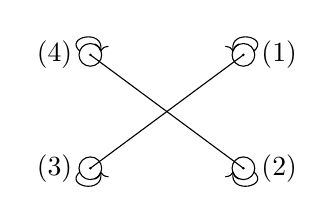
\begin{tikzpicture}[scale=0.72,baseline=(current bounding box.center)]
  \coordinate (a) at (-1.35,1.0);
  \coordinate (b) at (1.35,1.0);
  \coordinate (c) at (-1.35,-1.0);
  \coordinate (d) at (1.35,-1.0);
  \draw (a)--(d);
  \draw (c)--(b);
  \foreach \p/\lab/\pos in {a/{(4)}/left,b/{(1)}/right,c/{(3)}/left,d/{(2)}/right}{
     \draw (\p) circle (0.20);
     \fill (\p) circle (0.025);
     \node[\pos=3pt] at (\p) {\lab};
  }
  \draw[->] ($(a)+(-0.18,0.06)$) .. controls ($(a)+(-0.48,0.32)$) and ($(a)+(0.25,0.47)$) .. ($(a)+(0.18,0.06)$);
  \draw[->] ($(b)+(0.18,0.06)$) .. controls ($(b)+(0.48,0.32)$) and ($(b)+(-0.25,0.47)$) .. ($(b)+(-0.18,0.06)$);
  \draw[->] ($(c)+(-0.18,-0.06)$) .. controls ($(c)+(-0.48,-0.32)$) and ($(c)+(0.25,-0.47)$) .. ($(c)+(0.18,-0.06)$);
  \draw[->] ($(d)+(0.18,-0.06)$) .. controls ($(d)+(0.48,-0.32)$) and ($(d)+(-0.25,-0.47)$) .. ($(d)+(-0.18,-0.06)$);
\end{tikzpicture}
\end{equation}
Prenons comme point base le point fixe $z=0$ de $\sigma$. Le groupe fondamental $\pi_1(P-S,0)$ est engendré par les lacets $\gamma_i$ ($i\in\Z/4$) représentés en (7.6.1), avec $\gamma_1\gamma_2\gamma_3\gamma_4=1$ pour seule relation, et $\sigma$ envoie $\gamma_i$ sur $\gamma_{i+2}$.

Donner un système local $\mathcal V$ sur $P-S$ revient à donner sa fibre $\mathcal V_0$ en $0$ et l'action de $\pi_1(P-S,0)$ sur celle-ci. Soit $A_i$ l'image de $\gamma_i$. Pour notre $\mathcal V$, si l'on choisit un isomorphisme de $\mathcal V_0$ avec $\C^2$, la représentation de $\pi_1$ est donnée par quatre matrices $A_i$ dans $\SL_2(\C)$ vérifiant
\begin{equation}\tag{7.6.2}
A_1A_2A_3A_4=1.
\end{equation}
Nos hypothèses sont que la représentation est irréductible et que $A_i$ est conjuguée à $A_{i+2}$. Nous affirmons que les quadruplets $(A_1,A_2,A_3,A_4)$ et $(A_3,A_4,A_1,A_2)$ sont conjugués, autrement dit que les représentations correspondantes de $\pi_1$ sont isomorphes. Pour cela, il suffit, par irréductibilité, de vérifier qu'elles ont le même caractère: pour tout mot $\prod_k A_{i(k)}^{\varepsilon(k)}$ dans les $A_i^{\pm}$,
\begin{equation}\tag{7.6.3}
\Tr\prod_k A_{i(k)}^{\varepsilon(k)}=\Tr\prod_k A_{i(k)+2}^{\varepsilon(k)}.
\end{equation}
Nous sommes en rang $n=2$. Par Procesi [P], théorème 3.4 (a), p. 316, appliqué aux $A_i$ et à leurs inverses, il suffit de vérifier (7.6.3) pour les mots de longueur $\le2n-1=3$. Les mots peuvent être considérés comme des mots circulaires. Par les identités $A_i^{-1}=\Tr(A_i)-A_i$ et $A_i^2=\Tr(A_i)A_i-1$, il suffit de considérer les mots en les $A_i$ pour lesquels deux $A_i$ consécutifs ont des indices distincts. Pour des mots circulaires de longueur $\le3$, cela signifie que tous les indices sont distincts. Vérifions maintenant (7.6.3) pour ces mots. Nous utiliserons que, dans $\SL(2)$, $\Tr(A)=\Tr(A^{-1})$.

Nous avons supposé $\Tr(A_i)=\Tr(A_{i+2})$. L'égalité $\Tr(A_iA_{i+2})=\Tr(A_{i+2}A_i)$ est claire. Par (7.6.2), on a
\[
\Tr(A_3A_4)=\Tr((A_1A_2)^{-1})=\Tr(A_1A_2)
\]
et de même pour $A_iA_{i+1}$. Le cas de $A_1A_2A_3$ se ramène à celui de $A_4$ par
\[
\Tr(A_1A_2A_3)=\Tr(A_4^{-1})=\Tr(A_4).
\]
Le cas de $\Tr(A_1A_3A_2)$ résulte de l'identité
\begin{equation}\tag{7.6.4}
\begin{aligned}
&\Tr(ABC)+\Tr(ACB)-\Tr(A)\Tr(BC)-\Tr(B)\Tr(CA)\\
&\hspace{3em}-\Tr(C)\Tr(AB)+\Tr(A)\Tr(B)\Tr(C)=0,
\end{aligned}
\end{equation}
qui provient de l'annulation de l'opérateur d'antisymétrisation $a=\sum\varepsilon(\tau)\tau$ de $(\C^2)^{\otimes3}$: on développe
\[
\Tr(A\otimes B\otimes C\circ a)=0.
\]
De même lorsque $(1,2,3)$ est remplacé par $(i,i+1,i+2)$. Ceci conclut la vérification requise.
\end{proofdel}

Supposons maintenant que $k$ soit un corps algébriquement clos quelconque, et considérons les faisceaux $\Ql$-lisses au sens \'{e}tale de 1.1.

\begin{corollary*}[7.7]
Pour $(P,S)/k$ comme ci-dessus, 7.6 reste valable pourvu que la monodromie locale soit modérée. Par conséquent, 7.5 reste valable.
\end{corollary*}

La modération est déjà nécessaire pour donner un sens à «monodromie locale conjuguée».

\begin{proofdel}[Preuve pour $k=\C$.]
La preuve de 7.6 est algébrique, donc vaut aussi pour les systèmes locaux d'espaces vectoriels sur $\Ql$ sur $P(\C)-S$. Il reste à observer que le foncteur
\[
(\hbox{faisceaux }\Ql\hbox{-lisses sur }P-S)\longrightarrow
(\hbox{systèmes locaux d'espaces vectoriels sur }\Ql\hbox{ sur }P(\C)-S)
\]
est pleinement fid\`ele. En effet, les deux catégories sont des 2-limites inductives de catégories analogues, avec $\Ql$ remplacé par une extension finie $E_\lambda$ de $\Q_\ell$ dans $\Ql$. Cela nous ramène au cas $E_\lambda$. Soit $\OO_\lambda$ l'anneau de valuation de $E_\lambda$ et fixons un point base $0$. Les systèmes locaux sur $P(\C)-S$ sont des représentations de $\pi_1(P(\C)-S,0)$ sur un $E_\lambda$-espace vectoriel de dimension finie. Les faisceaux $E_\lambda$-lisses sur $P-S$ sont les représentations $V$ qui s'étendent en représentations continues du complété profini de $\pi_1$, c'est-à-dire celles pour lesquelles $V$ contient un réseau $V^0$ (un sous-$\OO_\lambda$-module libre de $V$ qui engendre $V$ sur $E_\lambda$) stable par l'action. Les morphismes sont les mêmes.
\end{proofdel}

\begin{proofdel}[Preuve en caractéristique zéro.]
Ce cas résulte du cas $k=\C$, par invariance du $\pi_1$ algébrique lors de l'extension des scalaires d'un corps algébriquement clos de caractéristique zéro à un autre.
\end{proofdel}

\begin{proofdel}[Preuve en caractéristique $p$.]
Grothendieck a prouvé que le $\pi_1$ modéré est un quotient du groupe $\pi_1$ de caractéristique $0$. Nous montrons que sa preuve ramène le cas de caractéristique $p$ au cas de caractéristique zéro. Soit $W(k)$ l'anneau des vecteurs de Witt de $k$. Soit $\overline K$ une clôture algébrique du corps des fractions $K$ de $W(k)$. Considérons un relèvement $(P_W,S_W)$ de $(P,S)$ à $W(k)$. L'action de $V_S$ se relève. Un système local sur $\Ql$ sur $P_S$, modérément ramifié le long de $S$, se relève uniquement à $P_W-S_W$, puis se tire en arrière sur $(P_W,S_W)\otimes_W\overline K$. Par Grothendieck, le foncteur obtenu des systèmes locaux modérés sur $P-S$ vers les systèmes locaux sur $P_{\overline K}-S_{\overline K}$ est pleinement fid\`ele; cela nous ramène au cas de caractéristique zéro.
\end{proofdel}

\heading{7.8. Fin de la preuve de 7.1.} Définissons $(X'_1,S'_1)$ comme le tordu de $(X_1,S_1)$ par $t(S_1)$. Sur $\Fb$, nous avons un système naturel de quatre isomorphismes entre $(X,S)$ et $(X',S')$, échangés par le Vierergruppe. Par 7.5, ils induisent tous la même bijection de $\mathcal T^{(2)}(X,S)$ vers $\mathcal T^{(2)}(X',S')$. Par transport de structure, cette bijection est compatible avec l'action de $\Frob$. Il s'ensuit que
\[
T(X_1,S_1,2)=T(X'_1,S'_1,2).
\]
Le diviseur $S'_1$ contient un point rationnel. Pour $(X'_1,S'_1)$, on a donc $N_1\ge2$, et (7.1.1) pour $(X_1,S_1)$ résulte de (7.1.1) pour $(X'_1,S'_1)$.

En traduisant la généralisation 7.7 de 7.5 au moyen de la correspondance de Langlands globale [L], on obtient le résultat suivant, dont nous ne connaissons pas de preuve n'utilisant pas [L].

\begin{proposition*}[7.9]
Soit $S_1$ un diviseur \'{e}tale de degré quatre de $\mathbb P^1/\Fq$, et soit $\sigma$ un automorphisme involutif de $(\mathbb P^1,S_1)$ qui agit sur $S$ par un élément de $V_S$. Supposons que la représentation automorphe $\pi$ de $\GL(2,\Adele)$ soit cuspidale, non ramifiée hors de $S_1$, et que sa composante locale en chaque $s$ de $S_1$ soit de la forme
\[
\Stein\otimes\chi(\detm)
\]
où $\chi$ est non ramifié.

Sous ces hypothèses, $\sigma(\pi)$ est un tordu sur $\Fq$ de $\pi$: il existe un signe $\varepsilon=\pm1$ tel que $\sigma(\pi)$ soit le tordu de $\pi$ par le caractère $a\mapsto\varepsilon^{\operatorname{deg}(a)}$ du groupe des classes d'id\`eles. Par conséquent, pour tout point fermé $x\notin S_1$, la valeur propre de Hecke de $\pi$ en $x$ est $\varepsilon^{\operatorname{deg}(a)}$ fois la valeur propre de Hecke de $\pi$ en $\sigma(x)$.
\end{proposition*}

Le couple $(\mathbb P^1,S_1)$ admet une involution $\sigma$ comme en 7.9 dès que $S_1$ l'admet, c'est-à-dire sauf dans le cas où $S_1$ contient un point rationnel et un point de degré $3$.

\begin{proofdel}
Soit $\mathcal F_1$ le faisceau $\ell$-adique lisse sur $(\mathbb P^1-S_1)/\Fq$ attaché à $\pi$. Comme $\pi$ est cuspidale, $\mathcal F_1$ est irréductible. Sa monodromie locale en chaque $s\in S_1$ est unipotente principale. Par 1.9(i), son image inverse $\mathcal F$ sur $(\mathbb P^1-S)/\Fb$ est encore irréductible. Par 7.7, $\sigma^*\mathcal F$ est isomorphe à $\mathcal F$. Par 1.9(ii), $\sigma^*\mathcal F_1$ est un tordu sur $\Fq$ de $\mathcal F_1$. Il en résulte que $\sigma(\pi)$ est un tordu sur $\Fq$ de $\pi$: pour un certain caractère $\chi$ du quotient $\Z$ du groupe des classes d'id\`eles, $\sigma(\pi)=\pi\chi$. En appliquant $\sigma$, on obtient $\pi=\sigma(\pi)\chi$, et $\pi=\pi\chi^2$. Par 1.9(ii), $\chi^2=1$: $\chi$ est de la forme $\varepsilon^{\operatorname{deg}(a)}$ pour un certain signe $\varepsilon$.
\end{proofdel}

\section*{1. Appendice. Transfert de représentations automorphes spéciales}
\begin{center}Yuval Z. Flicker\end{center}

Le but de cet appendice est d'extraire de la littérature l'énoncé 11.3.

La correspondance qui relie les représentations automorphes $\pi'$ du spectre discret de toute forme intérieure $G'$ de $G=\GL(n)$ (groupe multiplicatif d'une algèbre simple de dimension $n^2$) aux représentations du spectre discret de $G$ est connue sans condition lorsque le corps de base est un corps de nombres $F$, par les travaux d'Arthur sur la formule des traces. Le cas où $\pi$ et $\pi'$ ont une composante cuspidale ([BZ]) en une place $v$ où $G'_v$ est $\GL(n,F_v)$ avait été prouvé dans [FK] (après des travaux antérieurs de [BDKV] et de [F1;III] sur $\pi,\pi'$ avec deux telles composantes), en utilisant la formule des traces simple de [FK]. Cette dernière méthode s'applique aussi lorsque le corps de base $F$ est un corps de fonctions, mais elle ne couvre pas le cas dont nous avons besoin, qui concerne les représentations automorphes $\pi'$ de $D^*(\Adele)$, où $D$ est une algèbre à division centrale sur $F$, telles qu'aucune composante $\pi'_v$ de $\pi'$ ne corresponde, par la correspondance locale, à une représentation cuspidale $\pi_v$ de $G_v=\GL(n,F_v)$.

Pour établir la correspondance dans le cas énoncé en 1.13, nous utiliserons la formule des traces pour $\GL(n)$ sur un corps de fonctions $F$, telle qu'elle a été développée par Lafforgue [Laf], où la formule est prouvée pour toute forme intérieure de $\GL(n)$. Le cas dont nous avons besoin est celui où, en deux places $v=v_1,v_2$ (notées $0$ et $\infty$ dans [Laf]), la fonction test $f=\otimes f_v$ (notée $h$ dans [Laf]) a une composante discrète $f_v$. Une fonction test (localement constante à support compact) $f_v$ est dite discrète si, pour tout sous-groupe parabolique standard propre $P=MN$ de $G=\GL(n)$, de radical unipotent $N$ et de sous-groupe de Levi standard $M$, elle satisfait l'identité
\[
\int_{K_v}\int_{N_v} f_v(k_v^{-1}m_vn_vk_v)\,dn_v\,dk_v=0
\]
pour tout $m_v\in M_v$. Un pseudo-coefficient discret de la représentation de Steinberg est construit dans [Lau], théorème (5.1.3), p. 133, après des travaux antérieurs de Kottwitz. En remplaçant $f_v$ par $g\mapsto\int_{K_v}f_v(k_v^{-1}gk_v)\,dk_v$, $K_v=\GL(n,\OO_v)$, nous pouvons supposer que $f_v$ vérifie $f_v(k_v^{-1}gk_v)=f_v(g)$ ($k_v\in K_v$, $g\in G_v$). Pour $f$ ayant une composante discrète $f_v$, la troncature ([Laf], pp. 225--227) est triviale.

Le théorème 10, p. 241, V.2.d, de [Laf] implique que, pour $f$ ayant deux composantes discrètes, le côté géométrique de la formule des traces se réduit à
\[
\int_{G(F)\backslash G(\Adele)/a^{\Z}}\sum_\gamma f(g^{-1}\gamma g)\,dg
=\sum_{\{\gamma\}}\int_{Z_G(\gamma)(F)\backslash G(\Adele)/a^{\Z}}\sum_\gamma f(g^{-1}\gamma g)\,dg,
\]
où la somme de gauche porte sur les éléments $\gamma$ de $G(F)$ dont le polynôme caractéristique est une puissance d'un polynôme irréductible, tandis que la somme de droite porte sur un ensemble de représentants des classes de conjugaison de tels $\gamma$ dans $G(F)$; $Z_G(\gamma)$ désigne le centralisateur de $\gamma$ dans $G$. Pour simplifier, nous pouvons choisir $f$ avec une composante $f_{v_3}$ qui s'annule sur l'ensemble singulier (l'ensemble des $\gamma$ ayant au moins deux valeurs propres égales). Comme on l'explique dans le dernier paragraphe ci-dessous, cela ne réduit pas l'applicabilité de nos techniques. Les $\gamma$ de la somme sont alors elliptiques réguliers (réguliers: valeurs propres distinctes): $F[\gamma]$ est une extension séparable de $F$ de degré $n$.

Cette somme est égale à la somme analogue pour la forme intérieure $G'$, enregistrée dans (2), p. 191, de [FK], pour des fonctions test correspondantes $f=\otimes f_v$ sur $G(\Adele)$ et $f'=\otimes f'_v$ sur $G'(\Adele)$. En particulier, $f_v=f'_v$ aux places $v$ où $G_v\simeq G'_v$, et $f_v,f'_v$ ont des intégrales orbitales correspondantes (pour tous les éléments réguliers $\gamma'$ de $G'_v$ et les $\gamma$ de $G_v$ ayant les mêmes polynômes caractéristiques; l'intégrale orbitale de $f_v$ en les éléments réguliers qui ne proviennent pas de $G'_v$ en ce sens est nulle, pour tout $v$). Remarquons que l'emploi du théorème 10, p. 241, V.2.d, de [Laf] est fait par commodité. La méthode des «fonctions sphériques $n$-admissibles» de [FK], p. 192, pourrait aussi être utilisée.

Pour une fonction test $f$ ayant une composante cuspidale (c'est-à-dire en une certaine place $v$, pour tout sous-groupe parabolique propre $P_v=M_vN_v$ de $G_v$, on a $\int_{N_v}f_v(xny)\,dn=0$ pour tous $x,y\in G_v$), l'opérateur de convolution $r(f)$ se factorise par la projection sur le spectre cuspidal. Le côté spectral de la formule des traces devient la somme $\sum_\pi m(\pi)\Tr\pi(f)$, où $\pi$ parcourt les classes d'équivalence des représentations irréductibles dans le spectre cuspidal de $G(\Adele)$, et $m(\pi)$ désigne la multiplicité de $\pi$ dans le spectre cuspidal ($m(\pi)$ est connu comme valant $1$ pour $G=\GL(n)$). Pour une fonction test générale $f$, qui peut ne pas avoir de composante cuspidale, il faut utiliser la décomposition spectrale de l'espace des formes automorphes et calculer le côté spectral de la formule des traces. Cela est fait dans [Laf], théorème 12, p. 309, VI.2.f, dans le cas dont nous avons besoin, à savoir $\GL(n)$ sur un corps de fonctions $F$.

Dans le cas des corps de nombres, Arthur a montré («propriété de scindage») que, pour une fonction test $f=\otimes f_v$ ayant deux composantes discrètes, le côté spectral se réduit à une somme discrète $\sum_\pi m(\pi)\Tr\pi(f)$, où $\pi$ parcourt les classes d'équivalence des représentations irréductibles $\pi$ dans le spectre discret de $G(\Adele)$, et $m(\pi)$ est la multiplicité de $\pi$ dans le spectre discret. Dans le cas des corps de fonctions, ceci n'a pas encore été fait; nous procédons donc autrement (et en fait nous déduisons ce résultat).

Fixons une nouvelle place $u$ ($\ne v_1,v_2$) de $F$. Supposons la composante $f_u$ sphérique ($K_u$-biinvariante). Notons $f_u^{\vee}$ la transformée de Satake de $f_u$. Alors le côté spectral, décrit par le théorème 12, p. 309, VI.2.f, de [Laf], est de la forme
\[
\sum_i c_if_u^{\vee}(t_i)+\sum_j\int_{\widetilde T_j}c_j(t)f_u^{\vee}(t)\,d_jt
\]
où les $c_i$ sont des nombres complexes, les $t_i$ appartiennent à l'espace compact de Hausdorff $\widetilde T$ défini dans les premières lignes de [FK], preuve du théorème 2, p. 197, les $\widetilde T_j$ sont des sous-variétés compactes de $\widetilde T$ (toutes les composantes irréductibles d'un $\widetilde T_j$ ont la même dimension $j$, $1\le j<n$), les $c_j(t)$ sont des fonctions à valeurs complexes sur $\widetilde T_j$, mesurables relativement à une mesure bornée $d_jt$ sur $\widetilde T_j$ ayant la propriété que $\vol(\widetilde T_{\varepsilon}(t))/\varepsilon$ est uniformément borné en $\varepsilon$ (voir [FK], premier paragraphe de la preuve de la Proposition, p. 198), et
\[
\sum_i |c_i|+\sum_j\sup_{t\in\widetilde T_j}|c_j(t)|+\sum_j\int_{\widetilde T_j}|c_j(t)|\,|d_jt|
\]
est finie.

La formule des traces affirme maintenant que le côté spectral est égal au côté géométrique de la formule des traces. Comme nous l'avons vu ci-dessus, le côté géométrique est une somme d'intégrales orbitales (pour $f$ avec $f_{v_1},f_{v_2}$ discrètes). Pour des fonctions test correspondantes $f$ et $f'$, les côtés géométriques des formules des traces pour $f$ sur $G(\Adele)=\GL(n,\Adele)$ et pour $f'$ sur $G'(\Adele)=D^*(\Adele)$ sont égaux. Donc les côtés spectraux sont égaux. Comme il est bien connu (voir, par exemple, [FK], Proposition, p. 191), le côté spectral dans le cas anisotrope (où $G'=D^*$) est discret: il est de la forme $\sum_i c'_if_u'{}^{\vee}(t'_i)$. Nous combinons cette dernière somme avec la somme $\sum_i c_if_u^{\vee}(t_i)$, pour de nouveaux $c_i$. La Proposition de la p. 198 de [FK], préparée précisément pour une situation comme la présente, implique que tous les nouveaux $c_i$ sont nuls (à savoir $c'_i=c_i$ et $t'_i=t_i$).

Nous concluons que, pour une fonction test $f=\otimes f_v$ ayant deux composantes discrètes, le côté spectral, tel qu'il est décrit par le théorème 12, p. 309, VI.2.f, de [Laf], se réduit à une somme discrète. Alors, pour des fonctions test correspondantes $f=\otimes f_v$ sur $G(\Adele)=\GL(n,\Adele)$ et $f'=\otimes f'_v$ sur $G'(\Adele)=D^*(\Adele)$, on a l'identité
\[
\sum_\pi m(\pi)\Tr\pi(f)=\sum_{\pi'}m(\pi')\Tr\pi'(f'),
\]
où la somme de gauche (resp. de droite) parcourt les classes d'équivalence des représentations irréductibles $\pi$ (resp. $\pi'$) dans le spectre discret de $G(\Adele)$ (resp. $G'(\Adele)$), et où $m(\pi)$ (resp. $m(\pi')$) désigne la multiplicité de $\pi$ (resp. $\pi'$) dans le spectre discret.

Un argument standard d'«indépendance linéaire généralisée des caractères» implique qu'en fixant une représentation $\pi_0^S=\otimes_{v\notin S}\pi_{0v}$ de $G(\Adele^S)=G'(\Adele^S)$, où $S$ est l'ensemble des places de $F$ telles que $G'_v\simeq G_v$ pour tout $v\notin S$, les sommes sur $\pi$ et $\pi'$ peuvent être prises sur les sous-ensembles de $\pi$ tels que $\pi_v=\pi_{0v}$ et de $\pi'$ tels que $\pi'_v=\pi_{0v}$ pour tout $v\notin S$. Le théorème de rigidité («théorème de multiplicité un fort») implique que la somme sur $\pi$ se réduit à au plus un terme (avec $m(\pi)=1$, par le théorème de multiplicité un pour $\GL(n)$).

Puisque dans notre cas $D$ est une algèbre à division, un résultat de Godement--Jacquet peut être utilisé comme dans [F2] pour montrer que la somme sur $\pi'$ est finie. Comme il est expliqué dans [F2], en utilisant des fonctions correspondantes $f_v$ sur $G_v$ et $f'_v$ sur $G'_v$, pour $v\in S$, qui sont supportées seulement sur l'ensemble régulier (en particulier nous pouvons utiliser $f_{v_3}$ comme ci-dessus), l'indépendance linéaire des caractères implique des relations de caractères entre $\pi_v$ et $\pi'_v$ pour tout $v\in S$. Le caractère détermine uniquement $\pi_v$ et $\pi'_v$, puisqu'il est localement intégrable (un analogue en corps de fonctions de ce résultat de Harish-Chandra en caractéristique $0$ a été prouvé par Lemaire [Le]). Ceci implique la correspondance dont nous avons besoin: si $\pi$ est une représentation cuspidale de $G(\Adele)$ dont les composantes en $v\in S$ sont Steinberg tordues par un caractère non ramifié, il existe exactement une (donc $m(\pi')=1$) représentation cuspidale $\pi'$ de $G'(\Adele)$ avec $\pi'_v\simeq\pi_v$ pour tout $v\notin S$. Alors $\pi'_v$ correspond à $\pi_v$ par la correspondance locale; ainsi $\pi'_v$ est un caractère non ramifié de dimension un pour tout $v\in S$. Réciproquement, étant donnée une représentation cuspidale $\pi'$ avec $\dim\pi'>1$, il existe une unique $\pi$ correspondante.

\section*{Remerciement}
Le second auteur remercie la Humboldt Stiftung à la HU de Berlin, le MPIM-Bonn, le SFB de Bielefeld, l'Université hébraïque, le Newton Institute à Cambridge et l'IHES pour leur soutien pendant la préparation de ce travail.

\section*{Références de l'appendice}
\begin{description}[leftmargin=2.7em,labelwidth=2.4em,style=nextline]
\item[{[BDKV]}] J. Bernstein, P. Deligne, D. Kazhdan, M.-F. Vigneras, \emph{Représentations des groupes réductifs sur un corps local}, Travaux en Cours, Hermann, Paris, 1984.
\item[{[BZ]}] J. Bernstein, A. V. Zelevinsky, \emph{Representations of the group $\GL(n,F)$, where $F$ is a local non-Archimedean field}, Uspekhi Mat. Nauk 10 (1976), 5--70.
\item[{[F1]}] Y. Flicker, \emph{Rigidity for automorphic forms}, J. Analyse Math. 49 (1987), 135--202.
\item[{[F2]}] Y. Flicker, \emph{Transfer of orbital integrals and division algebras}, J. Ramanujan Math. Soc. 5 (1990), 107--122.
\item[{[FK]}] Y. Flicker, D. Kazhdan, \emph{A simple trace formula}, J. Analyse Math. 50 (1988), 189--200.
\item[{[Laf]}] L. Lafforgue, \emph{Chtoucas de Drinfeld et conjecture de Ramanujan--Petersson}, Astérisque 243 (1997), ii+329 pp.
\item[{[Lau]}] G. Laumon, \emph{Cohomology of Drinfeld Modular Varieties}, Part I; Cambridge Studies in Advanced Math. 41, Cambridge Univ. Press, 1996.
\item[{[Le]}] B. Lemaire, \emph{Intégrabilité locale des caractères-distributions de $\GL_N(F)$ où $F$ est un corps local non-archimédien de caractéristique quelconque}, Compos. Math. 100 (1996), 41--75.
\end{description}

\section*{Références}
\begin{description}[leftmargin=2.7em,labelwidth=2.4em,style=nextline]
\item[{[BT]}] F. Bruhat, J. Tits, \emph{Groupes réductifs sur un corps local I, II}, Publ. Math. IHES 41 (1972), 5--251 and 60 (1984), 197--376.
\item[{[C]}] W. Casselman, \emph{A new non unitary argument for $p$-adic representations}, J. Fac. Sci. U. Tokyo 28 (1982), 907--928.
\item[{[D]}] V. Drinfeld, \emph{The number of two dimensional irreducible representations of the fundamental group of a curve over a finite field}, Funktsional Anal. i Prilozhen. 15 4 (1981), 75--76.
\item[{[K]}] R. E. Kottwitz, \emph{Tamagawa numbers}, Ann. of Math. 129 (1988), 629--646.
\item[{[Ko]}] M. Kontsevich, \emph{Notes on motives in finite characteristic} (arXiv:math/0702206v2).
\item[{[L]}] L. Lafforgue, \emph{Chtoukas de Drinfeld et correspondance de Langlands}, Inv. Math. 147 1 (2002), 1--241.
\item[{[O]}] T. Ono, \emph{On Tamagawa numbers}, in Algebraic groups and discontinuous subgroups, Part 1, 122--132, Proc. Symp. Pure Math. IX (1966).
\item[{[P]}] C. Procesi, \emph{The invariant theory of $n\times n$ matrices}, Adv. in Math. 19 (1976), 306--381.
\item[{[S]}] J.-P. Serre, \emph{Cohomologie des groupes discrets}, Ann. of Math. St. 70, 77--169, PUP; in: Oeuvres II, p. 593.
\end{description}

Institute for Advanced Study, Princeton, NJ 08540;\\
\emph{Adresse électronique:} deligne@ias.edu

The Ohio State University, Columbus, OH 43210;\\
\emph{Adresse électronique:} yzflicker@gmail.com

\end{document}
